\documentclass[12pt,twoside,final,hidelinks]{ltthesis}
\usepackage{epsfig,bm,epsf,float,lsalike}

\usepackage{xspace}
\usepackage{relsize}
\usepackage{url}
\usepackage{boxedminipage}
\usepackage{amsmath}
\usepackage{pdfpages}
\usepackage{subfig}
\usepackage{needspace}
\usepackage{array}
\usepackage{palatino}
\usepackage{booktabs}
\usepackage{algorithm}
\usepackage{algorithmic}
\usepackage{rotating}
\usepackage{tablefootnote}
\usepackage{multirow}
\usepackage{amsmath}
\usepackage{amsfonts}
\usepackage{lipsum}
\usepackage{breqn}
\usepackage{listings}
\usepackage{amsthm}
\usepackage{amsmath}
\usepackage{graphicx}
\usepackage{fixme}
%\usepackage{natbib}
\usepackage{soul}
\usepackage{qtree}
%\usepackage{natbib}
\usepackage{bibentry}
\usepackage{tikz-dependency}

\usepackage{fancyhdr}

\pagestyle{fancy}
\fancyhf{}

\fancyhead[RO,LE]{\thepage}
\fancyhead[LO]{\leftmark}
\fancyhead[RE]{\rightmark}


\usepackage{xcolor}
\theoremstyle{definition}
\newtheorem{exmp}{Example}[section]
\usepackage{xcolor}
\usepackage{lipsum}

% Define macro for paper 
\newcommand\emnlpiv{EMNLP 2014 (\S\ref{sec:emnlp14})}
\newcommand\conllv{ConLL 2015 (\S\ref{sec:conll15})}
\newcommand\aclv{ACL 2015 (\S\ref{sec:acl15})}
\newcommand\emnlpv{EMNLP 2015 (\S\ref{sec:emnlp15})}
\newcommand\naaclvi{NAACL 2016 (\S\ref{sec:naacl16})}
\newcommand\emnlpvi{EMNLP 2016 (\S\ref{sec:emnlp16})}
\newcommand\eaclvii{EACL 2017 (\S\ref{sec:eacl17})}

\raggedbottom
\newcommand{\tofix}[1]{\hl{#1}}

% Table of contents max depth listed:
% 1 = section, 2 = subsection, 3 = subsubsection
\setcounter{tocdepth}{2}


\begin{document}

%\input{mathdefs} % my math definitions.


% UNDERLYING SPACING FOR WHOLE DOCUMENT:
% Single spacing: takes place of `draft' mode, without losing figures.
%\ssp
\hsp
% makes double-spaced: fg(for GSAS requirement, microfiche):
%\dsp


%% frontmatter.tex
%%

\title{Natural Language Processing for Resource-Poor Languages}
\author{Long Thanh Duong}
\degreemonth{Feb} % month final submission occurs.
\degreeyear{2017}
\degree{PhD}
\department{Computing and Information System}
\advisor{A/Prof. Steven Bird} % Category I added.
\secadvisor{Dr. Trevor Cohn} % Category I added.


\maketitle
\copyrightpage


\begin{abstract}



\end{abstract}




\newpage

\addcontentsline{toc}{section}{Table of Contents}
\tableofcontents

\listoffigures
\listoftables
%(Cut them for my personal thesis format).




% cccccccccccccccccccccccccccccccccccccccccccccccccccccccccccccccccccccccccc
\begin{citations}

\vspace{0.8in}

\ssp
\noindent
Large portions of chapter \ref{chap:uniTagger} have appeared in the
following paper:\\

\begin{quote}
\textbf{ Long Duong}, Paul Cook, Steven Bird, and Pavel
Pecina. 2013. Simpler unsupervised POS tagging with bilingual projections. In \textit{Proceedings
of the main conference 51th Annual Meeting
of the Association for Computational Linguistics (ACL 2013)}.
Association for Computational Linguistics,
Sofia, Bulgaria
\end{quote}


\end{citations}




\begin{acknowledgments}
I would like to thanks my supervisors, family and friends....

\end{acknowledgments}





%ddddddddddddddddddddddddddddddddddddddddddddddddddddddddddddddddddddddddddd
\dedication

\begin{quote}
\hsp
\em
\raggedleft

Dedicated to youse all.

\end{quote}


\newpage

\startarabicpagination

%%% end



\chapter{Introduction}
\label{chap:introduction}
% 0. NLP tasks and the need for annotated data,
Natural Language Processing (NLP) is an active field of research which aims, broadly speaking, to teaching computers to understand human language. Achieving that goal is not easy as the computer must understand many facets of language such as syntactic, semantics, and work with different input formats such as raw text, image and speech. Most NLP algorithms employ some form of machine learning techniques. Recently, many advancements in NLP have been realized thanks to more computing resources, better understanding of the algorithms and more annotated data. 

Solving a NLP task usually involves annotating a lot of data and then applying supervised machine learning algorithms. For example, if we are interested in part-of-speech (POS) tagging, we would imagine annotating each word in the sentence with the correct POS tag such as Noun, Verb, Adjective and then training a statistical classifier. In this approach, annotated data is crucial as it provides the only guidance for the model. In recognition of the importance of annotated data, annotated resources have long been a part of NLP conferences. Moreover, the Language Resources and Evaluation Conference (LREC) is a major conference dedicated to language resources. 

% Annotated data is important but expensive/tedious/slow/ to get ... 
% - for 1000 sentence in the parsing ... 
% - time consuming and money 
% - not task dependent 
Clearly, annotated data is gold, however, it is expensive and time-consuming to build. Annotation projects typically require careful design, testing, and subsequent refinement of annotator's guidelines, as well as quality assessment and management. For example, in the case of the Prague Dependency Treebank (PDT), it took a year to annotate the first 1000 sentences and 8 years to finish version 1~\cite{bohmovahhh:2001}. Moreover, annotated data is 
usually task specific, meaning that it cannot be reused for different purposes. In this fast changing field, sole reliance on annotated data is risky and not a good strategy. Thus, remedying this is one focus of this thesis. 

\begin{figure}
\centering
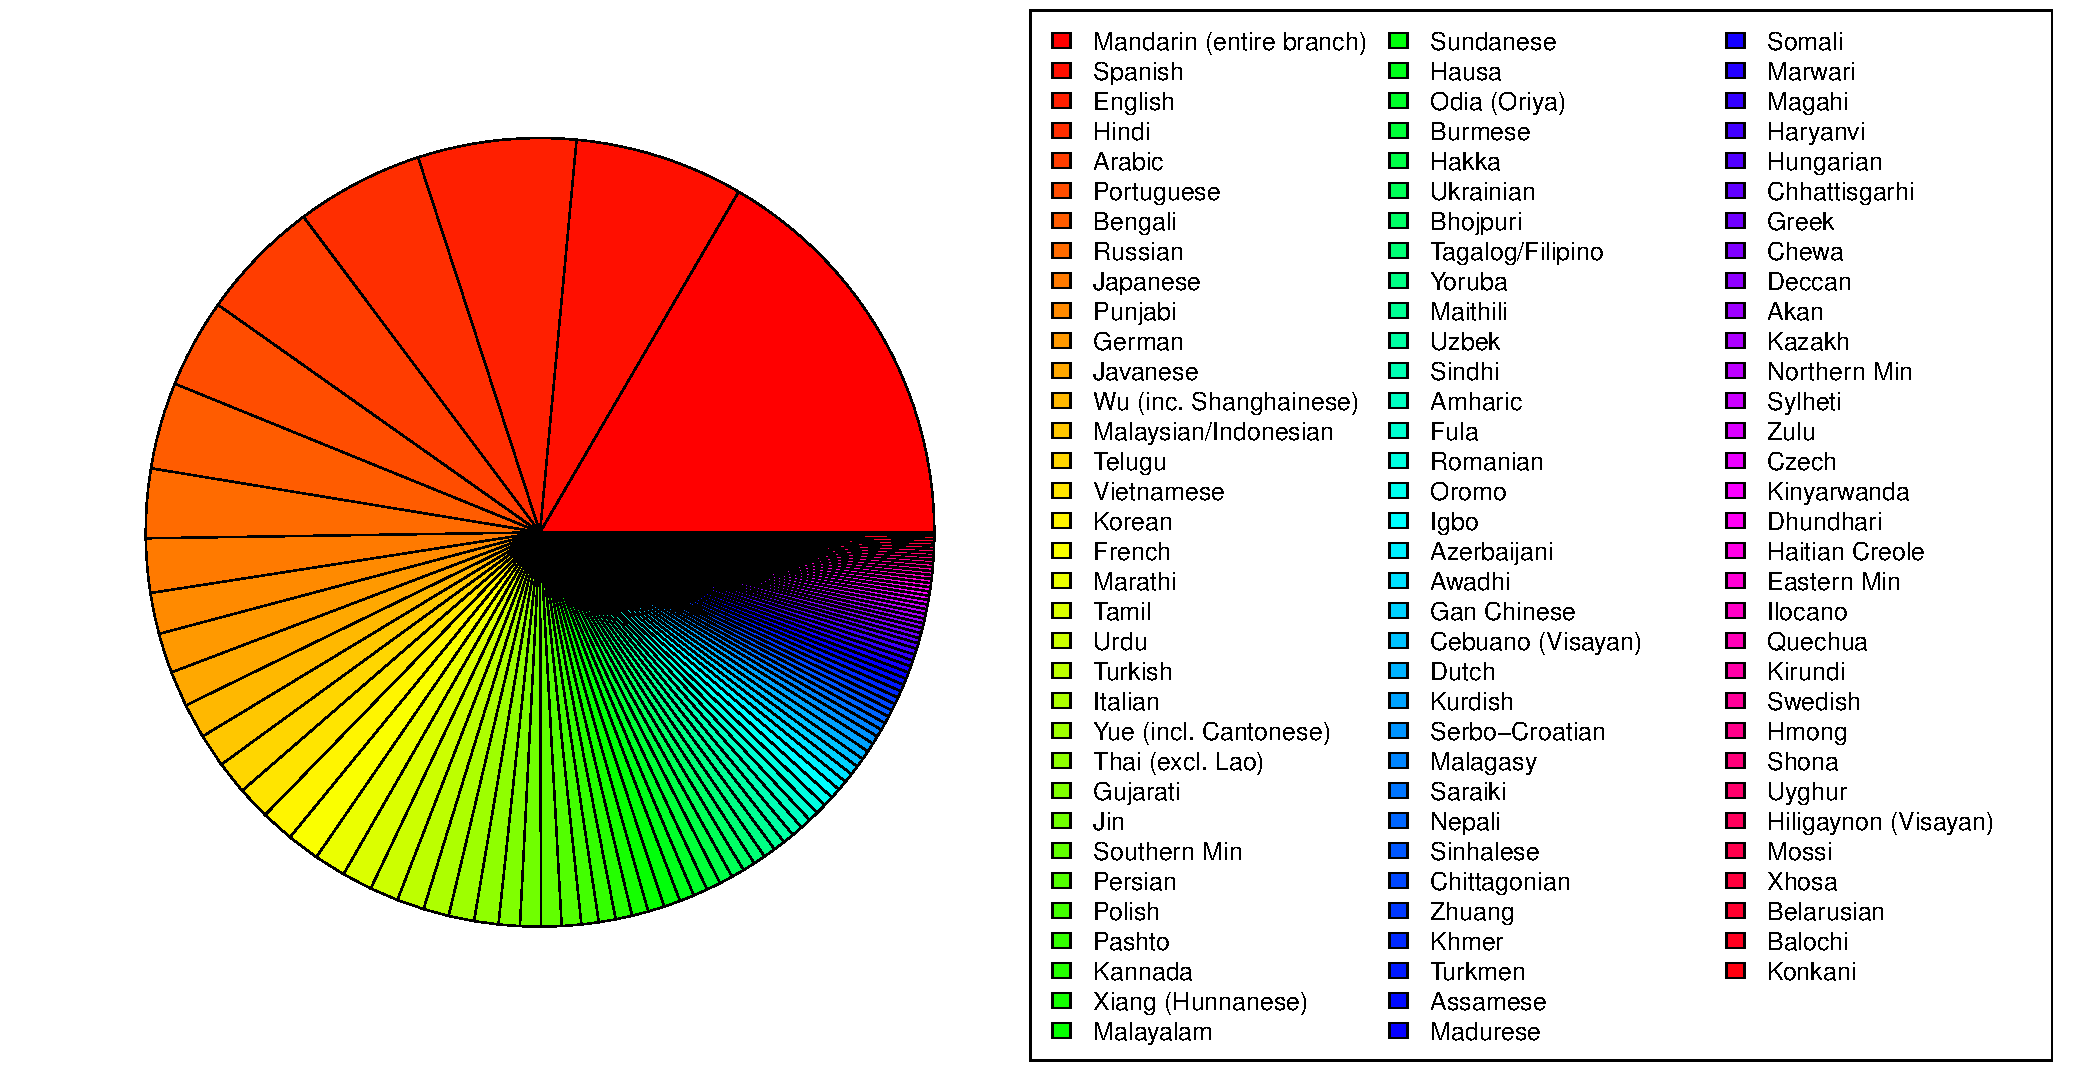
\includegraphics[scale=0.4]{Figures/ring_plot_languages}
\caption[Fraction of world population by number of native speakers]{Fraction of world population (percentage) by number of native speakers in 2007. This diagram should be viewed in color. [sourced Wikipedia]}
\label{fig:language_by_speakers}
\end{figure}
% Low-resource languages are not uncommon 
Since it is expensive and hard to get, most annotated data is in high-resource or resource-rich languages such as English, Mandarin and Portuguese. Doing NLP is much more challenging for so-called ``low-resource" or ``resource-poor'' languages for which available resources, particularly annotated data such as treebanks, wordnets, and the like, are limited~\cite{AbneyBird2010}. Standard supervised learning techniques require significant amount of annotated data which is not suitable for many low-resource languages. There are approximately 7,000 languages in the world, but of these only a small fraction (20 languages) are considered high-resourced~\cite{BAUMANN14}. 
Low-resource languages are in dire need of a method to overcome the resource barrier, such that advances in NLP can be realised much more widely. Figure~\ref{fig:language_by_speakers} shows the proportion of the world languages by number of native speakers. 
%Table \ref{tab:majorLanguageLessData} shows some major languages with no or very limited annotated data available. 
Despite the dearth of data, many languages are widely spoken such as Bengali, Punjabi, Javanese, Wu, Telugu and Vietnamese. Together, the low-resource languages shown in Figure~\ref{fig:language_by_speakers} %Table~\ref{tab:majorLanguageLessData} 
are spoken by almost 2 billion people, roughly a third of the world's population. 
% annotation to some degree 

% 3. Abundant of complementary resource... 
% - Parallel data 
% - Transfer learning ? 
Despite the lack of annotated data, even for low-resource languages there are some unannotated data which we can exploit in order to learn more accurate model. With the growing 
quantity of text available online, and in particular, multilingual parallel texts from sources such as multilingual websites, government documents and large archives 
of human translations of books, news, and so forth, unannotated parallel data is becoming more widely available. This parallel data can be exploited to bridge 
languages, and in particular, transfer information from a resource-rich language to a resource-poor language. 

Knowledge bases such as dictionaries, wordnets and 
other lexical resources are another sources of information, and exist in some form for many of the world's low-resource languages. The argument is that the 
manually annotated data is hard to get yet bilingual lexical resources are more widely available. For instance, the Wiktionary 
project\footnote{wiktionary.org} uses crowd-sourcing to build dictionaries in many languages using the collaborative efforts of volunteers. In this way the 
dictionary grows in both size and language coverage over time. Panlex is another example of multilingual dictionary that covers thousands of 
languages~\cite{Kamholz14}. However, these resources are limited to only lexical items without any deeper annotation. Clues from related languages can also compensate for the lack of 
annotated data, as we expect there to be information shared between closely related languages in terms of the lexical items, morphology and syntactic structure. In 
this thesis, we investigate the method for effectively harness these additional resources aside from annotated data aiming for complementary effect. 

% 4. Speech part of the language 
% Languages are dying and need to preserve
% Speech is a natural way of communication, need to upderstand speech for low-resource languages
% 
Out of the 7,000 languages, half of them do not even have the writing system and many are dying~\cite{lewis2009}. It is estimated that by the end of this century, 
half of the world's languages will become extinct as there are no speaker for that language~\cite{crystal2002language}. Since language captures knowledge and 
wisdom, more attention is given for preserving the language before it is lost forever.~\namecite{bird-EtAl:2014:W14-22} pioneer on using speech technology to 
preserve the language using their Android application called Aikuma which records speech in low-resource languages and translation in higher 
resource languages. They use speech translation as a way to preserve the language. However, it is unclear how to automatically process and learn from this collected 
data. This is one of the motivation for this thesis. 

%\begin{table}[h]
%  \centering
%    \begin{tabular}{lc|lc}
%    \textbf{Language} & \textbf{Speakers (M)} & \textbf{Language} & \textbf{Speakers (M)}\\
%	Bengali & 205   &   Burmese & 33 \\
%	Punjabi & 102   &  Hakka & 31 \\ 
%    Vietnamese & 90 &    Bhojpuri & 29 \\ 
%    Javanese & 85 & Tagalog & 28 \\
%    Lahnda & 82 & Yoruba & 28 \\
%    Wu & 80 &  Maithili & 27 \\
%    Marathi & 72 & Swahili & 26 \\ 
%    Tamil & 69 &    Uzbek & 26 \\ 
%    Urdu & 64 &    Sindhi & 26 \\ 
%    Gujarati & 49 &     Amharic & 25 \\ 
%    Jin & 48 &      Fula & 25 \\ 
%    Min Nan & 47 &  Oromo & 24 \\ 
%    Pashto & 39 &     Igbo & 24 \\ 
%    Kannada & 38 & Azerbaijani & 23 \\ 
%    Xiang & 38 &     Gan & 22 \\ 
%    Malayalam & 38 &   Cebuono & 21 \\ 
%    Sundanese & 38 &     Kurdish & 21 \\ 
%    Hausa & 34 &     Lao & 20 \\ 
%    Oriya & 33 &     ... & ...\\

%	\end{tabular}
%	 \caption{Major languages with little or no annotated data from \protect www.ethnologue.org (date accessed: 09/2014).}
%% CPC When citing a website, also give the date accessed.
%  \label{tab:majorLanguageLessData}%
%\end{table}	

\section{Research Questions}
Extending existing NLP methods to cater for low-resource languages is an active area of investigation. For these languages, the conventional approaches using supervised machine learning are inappropriate due to the lack of annotated data. Purely unsupervised approaches appear to be a better fit. However, despite considerable effort, their performance lags well behind supervised approaches, and is rarely adequate. A more pragmatic and fruitful research direction which is attracting much attention, is to exploit different sources of information aside from simple annotated text. In this thesis, we want to investigate different levels of resource requirement for low-resource languages ranging from semi-supervised and unsupervised learning to the extreme case of processing unwritten languages. Thus our research questions are: 
\begin{enumerate}
%\item What is the performance gap between supervised and unsupervised approaches? Answer this question will give overview about previous approaches and the current state-of-the-art which will be the point of comparison. 
%\item What is the realistic data assumption for low-resource languages ? 
\item How can we achieve more accurate models for low-resource languages using less annotated data? The assumption here is that annotated data is hard to get but other resources such as parallel data, monolingual text and bilingual dictionaries are more widely available, and can be used to further improve the performance.
\item How can we achieve more accurate models for low-resource languages without annotated data? The previous question still assumes some small amount of annotated data in the target language. However, this assumption does not always hold true.
\item What can we learn from unwritten languages? This question aims at solving the extreme case where we do not even have the writing system for a low-resource language.  
\end{enumerate}
These questions are arranged in order of increasing complexity by reducing resource requirements. Generally speaking, the first and second questions are about how to improve
the performance of semi-supervised and unsupervised learning applied to low-resource languages. The third question is particularly challenging as the resource requirements are minimized, concerning extremely low-resource unwritten languages. 

\section{Scope}
We aim at building an NLP framework for processing low-resource languages. However, due to the language complexity, it is hard to say when a language is sufficiently processed. Even for high-resource language such as English, there is no framework to truly and completely understand English. However, there are well-established NLP tasks for processing a language such as text summarization, part-of-speech tagging, coreference resolution, machine translation, named entity recognition, optical character recognition, natural language understanding, parsing, sentiment analysis, speech recognition, speech segmentation, text-to-speech, word segmentation, word sense disambiguation, question answering and natural language generation. 
% Syntac and semantic analysis is important 
Each task has different object and tackle different problems. However, they can be related to \textit{syntax} and \textit{semantics}. Some tasks such as part-of-speech tagging or parsing is purely about syntax, while word sense disambiguation is mainly about semantics. Nevertheless, most tasks such as machine translation or sentiment analysis need some knowledge of both syntax and semantics. It appears that to process a language we need at least some basic tools to analyse the syntactic and semantic aspect of that language. 
% Multimodal modal ... 
The other distinguishing feature between NLP tasks is the \textit{input format}. While many tasks process raw text, optical character recognition and speech processing take image and speech as input. It is highly desirable that a framework to process a language must be able to handle multiple input formats. Moreover, as mentioned before, many languages do not even have a writing system, and so directly processing speech is the only option. 
% 4 tasks. 
Given the time limitation of the research with respect to the syntactic and semantic aspect, and the requirement for multi-modal inputs and unwritten language processing, we focus on four NLP tasks:
\begin{enumerate}
\item Part-of-speech (POS) tagging which shows the syntax categories of lexical item, classifying words into POS categories such as noun, verb, adjective.
\item Dependency parsing which shows the dependency relationship between words in the sentence such as head/modifier and subject/verb. 
\item Cross-lingual word embeddings which represent lexical items from multiple languages in the same dense vector space, preserving the monolingual and bilingual property of the language. These embeddings would be the bridge between resource-rich and resource-poor languages allowing for transfer learning. 
\item Speech to text translation which learns the alignment and translation between speech in a low-resource language and the translation in the higher-resource language. This will be useful for tasks such as keyword spotting, and also relevant for unwritten language processing.  

\end{enumerate}

% Explain why select those 4 task 
These tasks are very related and the latter tasks are normally based on earlier one. 
The reason for choosing these tasks is mainly because they appear in most NLP pipelines and an advancement in NLP cannot be realized without recourse to these tasks. We cover both syntax (task 1 and 2) and semantics (task 3 and 4), and also attempt both text (task 1,2 and 3) and speech (task 4) representation of a language. Also, task 4 is dedicated mainly for processing unwritten language with a minimum resource requirement. By abusing the terms, we will also refer to task 4 as unwritten language processing task from herein. 

\section{Contributions}
% What are the contributions ? 
% Algorithms for better performance ? 
% Dataset 
% New tasks ? NAACL submission 
% EMNLP 2014 : POS tagging mapping tagset, resolve the different across languages. 
% ACL 2015: 
% EMNLP 2015 : Dependency parsing 
The main contribution is the algorithm it self. We propose several algorithms motivated by transfer learning and incorporate additional information to the model to improve performance. Moreover, we propose an algorithm based on deep neural networks to model unwritten language. The more detailed contributions are as follows:

\paragraph{POS tagging} We propose a semi-supervised method which incorporates noisy information from parallel data to the model as a prior. In this way, we 
demonstrate that only a mall amount of annotated data is sufficient in order to achieve a large improvement in performance. Compared with the state of the art system, 
which also take advantage of parallel data, we make more realistic assumptions and use less parallel data, while achieving a better overall result. 

The second contribution is the novel tagset mapping algorithm. The corpora we employed use mappings from language-specific POS tag inventories to a common universal tagset \cite{UniversalTagSet}. However, such a mapping might not be good, or even available, for resource-poor languages. Therefore, we propose a variant of our method capable of handling arbitrary tagsets based on a two-layer maximum entropy model. Evaluating on the resource-poor language Malagasy, we exceed the state of the art by a large margin. This work appeared as a long paper at \emnlpiv. 

\paragraph{Dependency Parsing} We propose a semi-supervised learning algorithm based on parameter sharing in a neural network parser. The additional information we incorporate to the model concerns the language relatedness. We show that a more accurate parser can be achieved using the same training data by taking reference from related model in different languages in the cascade style. This work is published as a short paper at \aclv. 

We realized that we can do this better by jointly training the model, instead of using the cascade approach. We jointly train a neural network dependency parser to model the syntax in both a source and target language. In this way, the information can flow back and forth between languages, allowing for the learning of a compatible cross-lingual syntactic representation, while also allowing the parsers to mutually correct one another's errors. 
Our experiments show that this outperforms a purely supervised setting, on both small and large data conditions, with a gain as high as 10\% for small training sets. 
Our proposed joint training method also out-performs the cascade approach mentioned earlier. The other contribution concerns the learned word embeddings.
We demonstrate that these embeddings encode meaningful syntactic phenomena, both in terms of the observable clusters and through a verb classification task. This part is published as a long paper at \emnlpv. 

In the extreme case where no annotated data is available, we propose an unsupervised dependency parser taking advantage of novel 
syntactic word embeddings. Words from both source and target languages are mapped to a shared low-dimensional
space based on their syntactic context, without recourse to parallel data.
While prior work has struggled to efficiently incorporate word embedding information into the parsing model~\cite{mohit:ACL14,andreas-klein:2014:P14-2,chen-zhang-zhang:2014:Coling},
we present a method for doing so using a neural network parser. When applied to the target language, we show consistent gains across all studied languages.
Moreover, when multiple source languages are available, we can attempt to boost
performance by choosing the best source language, or by combining
information from several source languages. To the best
of our knowledge, no prior work has proposed a means for selecting the
best source language given a target language. We
introduce two metrics which outperform the baseline of always picking
English as the source language. We also propose a method for combining
all available source languages which leads to substantial improvement in performance.
This work has been published as long paper at \conllv. 

\paragraph{Crosslingual Word Embeddings}
Crosslingual word embeddings represent lexical items from different languages in the same vector space, enabling transfer of NLP tools. 
However, previous attempts had %low-performance, 
expensive resource requirements, or difficulty incorporating monolingual data, or were unable to handle polysemy.
We address these drawbacks in our method which takes advantage of a high coverage dictionary in an Expectation-Maximization style training algorithm over monolingual corpora in two languages. Our model achieves state-of-the-art performance on bilingual lexicon induction task exceeding models using large bilingual corpora, and
competitive results on the monolingual word similarity and cross-lingual document classification task. We also evaluate several methods for combining embeddings which help in both crosslingual and monolingual evaluations. This work has been published as a long paper at \emnlpvi. 

We extend our work to cover more than two languages since most prior work on building crosslingual word embeddings focuses on a pair of languages.
English is usually on one side, thanks to the wealth of available English resources.
However, it is highly desirable to have a crosslingual word embeddings for many languages so that different relations can be exploited. We proposed novel algorithms for post-hoc combination of multiple bilingual word embeddings, applicable to any pre-trained bilingual model. We also extend our prior work to jointly learn multilingual word embeddings over monolingual corpora in several languages achieving uniformly excellent performance across a variety of tasks. This work has been accepted as a long paper at \eaclvii.

\paragraph{Unwritten language processing} For many low-resource languages, spoken language resources are more likely to be annotated with translations than 
transcriptions. This bilingual speech data can be used for word-spotting, spoken document retrieval, and even for documentation of endangered languages.
We experiment with the neural, attentional model applied to this data. On phone-to-word alignment and translation re-ranking tasks, we achieve large improvements 
relative to several baselines. On the more challenging speech-to-word alignment task, our model nearly matches GIZA++'s performance on gold transcriptions, but without recourse to transcriptions or to a lexicon.
Our main contributions are:
(i)~proposing a new task, alignment of speech with text translations, including a dataset extending the Spanish Fisher and CALLHOME datasets;
(ii)~extending the neural, attentional model to outperform existing models at both alignment and translation reranking when working on source-language phones; and
(iii)~demonstrating the feasibility of alignment directly on source-language speech. 
This part has been published as a long paper at \naaclvi. 

All in all, our contributions are:
\begin{itemize}
\item Showing how to effectively incorporate different information (such as parallel data, or language relatedness) to the model aside from annotated data. In many case, this helps not only resource-poor languages but also resource-rich languages. 
\item Analysing and tackling many real world low-resource scenarios such as annotation mapping and limited resource such as monolingual data, bilingual dictionary and speech recording. 
\item Showing the feasibility of learning meaningful relations directly from speech data and text translation in another language.
\item Proposing a new task of speech to text translation and creating several new datasets such as an English-Serbian bilingual lexicon induction dataset and a speech to text alignment corpus. 
\end{itemize}
\section{Thesis Overview}
%As the thesis goes, we plan to to answer the research question. 
The backbone of the thesis is the set of publications throughout the PhD candidature, addressing research questions. 
Chapter \S\ref{chap:background} lists the background needed to understand the thesis. Chapter \S\ref{chap:research_summary} enumerates the research outcome 
through a set of publications concerning all four tasks including POS tagging, dependency parsing, crosslingual word embeddings and unwritten language processing. 
With each publication, we will give an overview of research process and a retrospective view with an analysis of the strengths and weaknesses of each paper. Chapter \S\ref{chap:conclusion} conclude the thesis with a discussion of research questions, task coverage and future opportunities. 
%In the appendix we will discuss other papers related to the thesis that I contributed to but shouldn't be counted toward my PhD. 


%is about POS tagging for low-resource languages which cover our EMNLP 2014 papers. Chapter 4 is about dependency parsing for low-resource languages. This chapter is mainly by publications which are our ACL 2015, CoNLL 2015 and EMNLP 2015 papers. Chapter 5 is about crosslingual word embeddings which are also by publications which covers our EMNLP 2016 and COLING 2016 papers. Chapter 6 is about speech to text alignment which is also a chapter by publication cover our NAACL 2016 paper. In each chapter, 
%%% intro.tex
\chapter{Introduction}
%%%%%%%%%%%%%%%%%%%%%%%%%%%%%%%%%%%%%%%%%%%%%%%%
\label{section:intro}


\section{Part-of-speech Tagging}
% What is POS 
A Part-of-speech (POS) is the syntactic category of a lexical item (word). Lexical items which share the same POS are believed to have similar syntactic and morphological behavior. Common POS include Verb, Noun, Adjective, Pronoun, Adverb, Preposition and so forth. 
% Usage of POS 
POS information is used to disambiguate different syntactic categories. For example, in the sentence ``\emph{We can can a can}", the word ``\textit{can}" belongs to different categories: (1)~a modal verb, ie, \textit{somebody can do something}; (2)~a verb which is making a bottle; (3)~a noun which refers to a container. A POS tagger is a system for automatically determining the POS tag for a given text, and it should be able to distinguish syntactic categories by assigning tags to words. The above sentence can be tagged as ``\emph{We$_N$ can$_{MD}$ can$_V$ a$_{Det}$ can$_N$}" where \textit{N} is noun, \textit{MD} is modal verb, \textit{V} is verb, \textit{Det} is determiner. Another example is the word ``\textit{running}", the common interpretation is a verb i.e. ``\textit{he is running}". However, it could be an adjective i.e. ``\textit{running shoes}"  or noun i.e. ``\textit{running is good for health}". Therefore, sometimes POS tagging is also referred as choosing the right sense for the right context. Nevertheless, it is worth noting that when the same word-form has different tags, it will differ in meaning, but the reverse statement is not always true. For example, the word ``\textit{bank}" might refer to (1) the place where people conduct monetary transaction (2) the place near the river, but both meanings have the same ``\textit{Noun}" POS. 

POS tagging is one of the most basic operations of computational linguistic. Since it helps to disambiguate syntactic categories (and possibly senses), POS are regularly used in various natural language processing (NLP) tasks such as parsing, sentence classifying, word sense disambiguation and so-forth. 

\section{Tag set}
% Common tag set 
Tag set is the list of possible tags that a lexical item (word) can have. Normally, the tag set is different across languages. For English, the well-known tag set is Penn Treebank \cite{PenTreeBank} tag set which contains 48 tags; for more information please see Appendix \ref{section:appendixA}. The tag set is used to disambiguate morphology and syntax of lexical items. Therefore, the number of tags denotes the morphological complexity of a language. For example, there are 67 classes in the Prague Dependency Tree Bank \cite{HajicHajicovaAl2000} which shows the greater morphological complexity of Czech language compared with English. 
% Ref to apendix 
%\section{Formal definition}
%POS Tagger is the function $ f:A^+ \rightarrow T $ where $A$ is the alphabet of phonemes, $A^+$ denotes any non-empty sequence of phonemes. Normally, phonemes equal to letters. $T$ refers to tag set 
% Formal definition 
\section{Evaluation}
The most straightforward evaluation for POS tagging is \emph{per-token} accuracy. Firstly, sentence is tokenized, which will separate lexicon items from each other. Normally, space is used as the delimiter and period ``." indicates a sentence boundary. However, there are cases where this will not work, for example, the sentence \textit{``Mr. Peter ate a banana"} should be tokenized as \textit{(Mr.) (Peter) (ate) (a) (banana)} but not \textit{(Mr) (.) (Peter) (ate) (a) (banana)}. Second, the whole sentence is tagged. The tag of each token is then compared with the gold standard test data which is manually annotated by a linguist. The percentage of correctly tagged for tokens is known as the per-token accuracy. This measure is widely applied and has become the default evaluation. Supervised POS taggers achieve as high as 97 \% per-token accuracy for English~\cite{Toutanova:2003} and for many other languages. 

People might argue that this per-token accuracy is not meaningful because it takes into account punctuation marks and tokens that are not ambiguous. Therefore, another evaluation metric is  \emph{ambiguous-token} accuracy which only counts tokens that have more than one possible tag. The list of possible tags for each word can be acquired using dictionary or large manually annotated data. To the best of our knowledge, the best system \cite{Yoshida:2007} reports ambiguous-token accuracy around 87\%. 

Other evaluation is \emph{per-sentence} accuracy. That is, accuracy is calculated on the number of sentences for which all tokens are correctly tagged. This measure is more meaningful for tasks such as dependency-parsing where a single mistake in POS tagging might lead to completely wrong parsed sentence. The current good taggers report per-sentence accuracy around 55-57 \% \cite{Manning:2011:100}. 
In this thesis, we employ \textbf{per-token accuracy} for comparison purposes, thus, when we report accuracy of a tagger, we implicitly mean per-token accuracy. 

\section{Traditional approach}
The traditional approach to POS tagging builds a separate tagger for each target language. It does not take into consideration the relationship between languages. The supervised method which employs supervised machine learning algorithms is usually used. For each language they collect and build a large amount of manually annotated data and train a supervised POS tagger on it. The supervised style for the traditional approach has achieved very high tagging accuracy. The only issue is handling the out-of-vocabulary (OOV) case. The tagger is trained on labeled training data. However, there are cases where lexical items in test data are not present in training data. Therefore, we have very little information to predict the tag of an OOV word. The straightforward solution for the OOV is based on frequency of tags. That is assigning the highest frequency tag for the OOV word. More advanced solution might use the suffix/prefix of word or the prior tag sequences. For example, the suffix \textit{-ly} i.e. \textit{beautifully, quickly, lovely} etc, indicates an adverb, while the suffix \textit{-ive} i.e. \textit{attractive, possessive} indicates an adjective. Also, the information about tag sequences indicates that after determiner is usually a noun. 

\section{Challenges in POS tagging}
% Difficulty in POS tagging 
% Lack of data 
The first challenge for POS tagging is the training data. Currently, all supervised taggers outperform unsupervised ones. Supervised algorithms for POS tagger perform as accurate as 97\% for English~\cite{maximumEntropy}, French~\cite{denis:inria-00614819} and many other languages. However, supervised learning needs manually annotated data which is time consuming and costly to construct. There are approximately 7000 languages in the world but very small fraction (around 30 languages) have sufficient POS manually annotated data for building reliable supervised POS tagger. Unsupervised POS tagging, on the other hand, does not need any manually annotated data. It is more or less equivalent with unsupervised clustering task. That is, they tried to group words into syntactic cluster. The hypothesis is that words in the same cluster must share the same POS. However, there is a huge gap between supervised and unsupervised learning accuracy.  

% Lack of consensus between languages 
Current POS taggers are language oriented; there is a lack of consensus about the tagset. Tag set are adapted to each language, \textit{ an obstacle for cross-language processing}. For example, when calculating syntactic similarity between two languages, we need to compare tag sequence similarity. However, since tag sets for each language are different, they are incomparable. Another example is when working with a multilingual environment such as the World Wide Web, giving a solution that can work for every language is in high demand. However, if we keep individual tagsets for each language, we might have to manually or semi-automatically map tagsets between languages pairwise.  

\section{Universal Tagger}
% TODO : Introduce about 
In this thesis, we are going to investigate a solution to address the current challenges for POS tagging using a \emph{Universal Tagger}. Supervised styles, as mentioned above, are impossible for our Universal Tagger, which aims at building taggers not only for resource-rich but also for resource-poor languages. Completely unsupervised style is possible but low accuracy makes unsupervised POS tagger impractical. In this paper, we would like to investigate an unsupervised approach but additionally, exploit parallel data to copy tag information from resource-rich to resource-poor languages. Parallel data is acquired from a parallel corpus which contains many pairs of source sentences and their translation to the target language. We can use parallel data to bridge between languages and transfer annotated data from one language to the other. The intuition is that, for many resource-poor languages, there is no manually POS annotated data. Such data involves the intensive work of linguist, but parallel data is easier to acquire. 

The development of parallel data motivates us to build the Universal Tagger. Multilingual government documents, film subtitles, and a large amount of translation memory from books and news-papers, which are the source for parallel data, are becoming more and more widely available. Not only the size but also the language coverage of parallel data has improved drastically. The era of English dominating one side of parallel data is shifting to a far wider range of languages. 

Moreover, the Universal Tagger aims at pushing the boundary for cross-lingual natural language processing (NLP). Thus, the output of the Universal Tagger for each language must be comparable. To do this, we must employ the same tagset across languages. In this ways, we resolve the traditional ``language oriented" issues of the conventional POS tagger. 

\section{Main contributions}
In this thesis, we concentrate on the single task of unsupervised multilingual POS tagging (Universal  Tagger) which exploits parallel data. We give thorough reviews at related works on both traditional approach (monolingual) and modern approach (multilingual). We show both strong and weak points of these approaches in Chapter \ref{chap:backGround}. 

On Chapter \ref{chap:uniTagger} we are going to build a Universal Tagger which employs the consensus 12 Universal Tagset \cite{UniversalTagSet} which will enable cross-lingual comparison. Given a tagger for the source language and source-target language parallel data, we are able to build a tagger for the target language. We evaluate this on the same test data on the same 8 languages with the-state-of-the-art~\cite{Das:2011} using the same per-token accuracy metric. On average, our system performs on par with theirs but is penalized by using less data. Moreover, our method is much less sophisticated and runs much faster. 

Out of 8 languages, we perform better at 4 languages which are in the same language family tree (Germanic) with source language (English). This fact motivates us for Chapter \ref{chap:sourceLanguageSelection} which we dedicate for investigating the effectiveness of choosing different source languages. It turns out that English is rarely the best source language for many cases. We are also able to build a model that can predict the best source language just based on monolingual data. This model performs better than always fixing a single best source language. The further accurate prediction can be acquired if we additionally use multilingual data from the parallel corpus. Finally, we show that, if multiple source languages are available we can even get further improvement by incorporating information from multiple source languages.

Chapter \ref{chap:conclusion} contains the conclusion and a discussion of future work. We organize future work into different categories chronologically. That is: (1)~immediate work which might take few weeks to finish; (2)~near future work which might take a few months, and (3)~longer future work which might take years. 


\chapter{Background}
\label{chap:background}
% The importance of resources 
% Resource connect with performance 
% Resource is expensive 
% Literature is usually ignore the sarce of resource 
In this chapter, we will give the overview of low-resource natural language processing including definitions, datasets, common techniques and a high level reviews of related work. We then give the backgrounds of four tasks which will be investigated in this thesis. 

\section{Low-resource Natural Language Processing}
\subsection{Definition}
% No clear definition of what is low-resource languages.
Low-resource languages recently attract much attention, however we haven't given 
any concrete definition for low-resource languages. According to LORELEI,~\footnote{Low Resource Language for Emergent Incidents (LORELEI) is a US government funded project aiming at developing 
human language technology for low-resource languages} low-resource 
languages can be defined as  languages that no automated human language technology exist. 
However, the term human language technology is vague. Developing from this definition 
we refine the definition by picking an essential NLP task such as syntactic parsing as the yardstick. 
We instead can define a low-resource language as the 
language that does not have any syntactically annotated corpus which is essential 
to train the syntactic parser. Dependency treebank is popular among syntactically annotated corpora. 
Universal dependency treebank~\cite{11234/1-1699} 
is the largest collection of dependency treebanks in multiple languages currently 
covers 40 languages. Thus we can consider languages outside of those 40 languages, low-
resource languages. However, with this definition, it is arguable that can we use a single syntactic task such as 
syntactic parsing to represent language technology. Moreover, some languages (such as Buryat, Coptic, Kazakh, Sanskrit or Tamil) in those 40 languages have very modest size (less than 1000 annotated sentences). Dependency parsers trained on those treebanks would, expectedly, achieve 
modest performance. On the other end,~\namecite{berment:tel-00006313} proposed an extensive list of basic language resource kit for 
measuring language resources taking into consideration the minimum set of corpora, tools and human resources. They define a language is 
low-resource if the weighted score is less than a threshold. However, as expected, this definition is also heuristic as criticized by~\namecite{prys2006blark} by lack of consideration for raw material such as newspapers. 
We take the middle ground approach by simplify the definition of~\namecite{berment:tel-00006313}. 
We, instead, define low-resource languages taken into account the task. 
\begin{quote}
\textit{A language is considered low-resource for a given task if there is no algorithm using currently available data to automatically do the task 
with adequate performance.}
\end{quote}
% Language specific implication 
This definition implies that a language is considered low-resource based on the task. 
For example, Spanish is not low resource language with respect to 
the part-of-speech tagging task with a decent performance. However, it is 
resource poor language for sentiment analysis task 
since  there is not any annotated data for this task in Spanish. 
% Different gerer in one langauge can be consider low-resource languages
Different domain or genre inside a language can also be considered low-resource 
language. Taking POS tagging task as an example, the annotated corpus is mainly 
constructed for news wire domain, the accuracy of English tagger on this domain 
can be as high as 97\%~\cite{Toutanova:2003}. However, for historical English 
domain we achieve much lower accuracy~\cite{yang-eisenstein:2016:N16-1}. In this way, 
historical English domain becomes low-resource language given POS tagging task. 
% Large scope 
With this definition, the scope of this thesis is much bigger than low-density or indigenous languages. 
This is because for a given task requirement, many languages become low-
resource regardless of the number of speakers or the popularity.%, boosting the applicability of our approaches.  

% Low-resource today but no longer tomorrow. 
Moreover, it also should be noted that a language or domain is low-resource today but might not be in the future. English Twitter text is an example. It was resource-poor language 5 years ago without any tool to process. However, with the high demand on social data analysis, alot of research are poured into  building resources and models to effectively normalized the text, POS tagging, dependency parsing and sentiment analysis~\cite{han-baldwin:2011:ACL-HLT2011,gimpel-EtAl:2011:ACL-HLT2011,kong-EtAl:2014:EMNLP2014,Agarwal:2011:SAT:2021109.2021114} which makes English Twitter text no longer low-resource languages for those tasks. Our thesis is all about improving the performance to meet the expectation, leveraging the low-resource scenario. However, instead of looking at each domain (e.g. Twitter) or language individually, we want to investigate on the algorithm part such that it can widely be applied to many low-resource languages.   

\subsection{Language resources}
% Scale for languages given resources 
%High resource > Low resource (parallel data, some annotated data...) > Very low-resources (monolingual data...) > Remote language > Endanger language. 
Understanding what resource available is the first step to build the natural language processing framework for a target 
low-resource language. In general, we can classify languages into several categories according to the their language resources, in the  decending order of resources such as (1) High resource languages where there is decent-sized annotated data. This language category, however, falls out of scope of this thesis. (2) Low-resource languages where there is small-sized annotated data (3) Very low-resource languages where no annotated data is available but there are some bilingual resources such as dictionaries or parallel corpora and (4) Extremely low-resource languages where the data is mostly come from field linguists. Moreover, majority of languages in this category do not even have the writing system, adding complexity to this category. 
This section speculates the type of resource we can reasonably expect in the real world low-resource scenario. 
\subsubsection{Field linguist annotation}
Half of the world 7000 languages are unwritten languages~\cite{lewis2009}. It is the 
extreme case where the resource for those languages are usually come from field 
linguist annotations under language preservation and documentation projects. There can 
be many outputs from field linguist analysing some aspects of the language such that 
lexicon, morphology, phonology. However, it is usually unsuitable for 
automated natural language processing method because of the tiny size. 
Recently,~\namecite{bird-EtAl:2014:W14-22} proposed a new method to document a language using cheap mobile phone device through their application called 
Aikuma. This enable much faster and cheaper way for collaborative language documentation. The output from Aikuma is the parallel speech between the source low-resource and the target higher-resource 
languages with the options of re-speaking for higher quality record and some 
transcription in the target language. For the initial experiment,~\namecite{bird-EtAl:2014:Coling} managed to collect around 10 hours of speech from indigenous 
communities in Brazil and Nepal.~\namecite{Blachon201661} used an extended version of Aikuma to collect more than 80 hours of speech from Congo-Brazzaville. Thus, for the unwritten language, using Aikuma probably we can expect an order of 100 hours of parallel speech. 

\subsubsection{Monolingual Corpora} 
For the other half of the 7000 languages, we have some writing system. To cheaply collect the examples of a language (monolingual data), World Wide Web is probably the best option. 
%Moreover, thank to the World Wide Web, the monolingual data for a low-resource language/domain is now easier to get. This is normally the cheapest form of resource we can get.
% Website, project where we can get resource 
The Cr\'ubad\'an project~\cite{Scannell07thecrubadan} is an attempt to crawl
 monolingual data for resource-poor languages, to date they managed to support more than 2000 languages\footnote{crubadan.org (accessed 14/09/2016)}. Wikipedia is
  another major source for monolingual data contributed by volunteers, covering for more than 200 languages. Leipzig Corpora Collection (LCC)~\cite{GOLDHAHN12.327.L12-1154} is another project for
   collecting monolingual data which currently covers more than 200 languages, crawled from the web. 
However, we can expect very different monolingual data size for each language. For example, from Wikipedia, to date, 58 languages have more than 100k articles and 132 languages have more than 10k articles\footnote{en.wikipedia.org/wiki/List_of_Wikipedias (accessed 14/09/2016)}.
\namecite{GOLDHAHN12.327.L12-1154} shows that in LCC corpus at 2012, around 50 languages have 1 millions sentences and 100 languages have 70k sentences. That is why when working with languages in the top 50, probably we can expect the order of millions sentences or (10 million words). 

% Why a language is low-resource 
%A language is low-resource is mostly because of social, political and financial reasons. There might be not enough funding to attract research for that language. 
%As such, not much attention is given for that language. Consequently, it lacks the research, 

%When a language is low-resource, it means that 
% What it means by low-resource 
% What is resources here 

% This definition is because resource  connect to performance .... 
% Also means that no enough funding ... to attract research on that field. 
\subsubsection{Comparable and Bilingual Corpora}
Monolingual data only contain the relationship between lexical items inside a language. Comparable or bilingual corpora, on the other hand, can relate languages together. 
As the development of multilingual news, books, subtitles, government websites, it is easier to get the comparable corpora for many low-resource languages. They contains set of documents in multiple languages that is topically ``comparable''. Wikipedia is a source for comparable data since one topic (e.g. Barack Obama) is usually written in several languages. Multilingual online news service such as BBC\footnote{bbc.com (accessed 14/09/2016)} is another source for comparable data, available in 32 languages. STRAND~\cite{Resnik:2003:WPC:964751.964753} is the system to crawl comparable documents from the web based on the structure of the website. Their proposed system can be used to crawl comparable corpora for any language pair. However, as admitted, they could not find many language pairs and modest in size. 
%That is why for comparable corpora, probably we can get the decent size only for the
% mention STRAND 

Bilingual corpora is usually extracted from comparable corpora, representing sentence 
aligned translations. Bilingual corpora are particularly of interest since they are the 
main input for machine translation and can be used as the bridge between languages. 
Europarl~\cite{europarl} is a popular bilingual corpus covered many European languages 
as legal documents and policies are needed to translate to all 
participating country's languages. Opus~\cite{TIEDEMANN12.463.L12-1246} is an open-access platform 
for retrieving bilingual corpora, data is manually collected from many open
 multilingual sources such as movie subtitle, bible, European documents. Opus, probably,  is the
 largest collection of freely available parallel corpora, covered more than 90 
 languages. Each pair in the top 100 language pairs in Opus has more than 100 million 
 words. This is a decent size even for resource intensive NLP. However, most of the 
 top 100 language pairs are from well-supported languages with some 
 exceptions such as Romanian-Turkish and Bulgarian-Hungarian. That is why for low-resource languages, we can not expect that much of parallel data which is usually overlooked by previous work. 
% Not realistic assumption for parallel data for many works
%Many previous approaches for low-resource NLP rely on parallel data as the bridge to 
%transfer the annotation from the source resource-rich language to the target resource-poor 
%language~\cite{Das:2011,Duongacl13}. 
In addition, due to lack of the 
evaluation data for real low-resource languages, previous work usually evaluate on simulated scenario on well-supported 
languages. Consequently, the parallel data is much easier to get for those languages. 

How much parallel data can we reasonably expect for a low-resource language? It is hard to 
estimate and will be different according to language. However, if we are working with top 15 
languages ($\approx100$ pairs) which mainly are European languages, probably we can get a 
decent parallel size, in order of million sentence pair. Nevertheless, in our \emnlpiv\ paper, 
we experimented with two low-resource languages, Malagasy and Kinyawanda. The biggest bilingual 
corpora we can find are in order of 100k and 10k sentences respectively.


% START FROM HERE 




\subsubsection{Bilingual Dictionary}
Bilingual dictionary is a common resource for a low-resource language. This is usually the output of linguist when one language is studied. Bilingual dictionary contains the word translation of a low-resource language to the more common language such as English. 
There are some notably corpus that collect translation for multiple languages. 
Panlex~\cite{Kamholz14}, a dictionary which currently covers around 1300 language varieties with about 12 million expressions\footnote{an expression is usually a word in a language.}. This dataset is growing and aims at covering all languages in the world and up to 350 million expressions. 
The translations in PanLex come from various sources such as glossaries, dictionaries, automatic inference from other languages, etc. 
Accordingly, Panlex has high language coverage but often noisy translations.
Wiktionary~\footnote{en.wiktionary.org (accessed 19/09/2016)} is another notable source for bilingual dictionary. A part of Wiktionary 
is also manually extracted from dictionaries and glossaries but it is also powered by 
volunteers. Currently, Wiktionary covers over 2500 languages\footnote{However, more than 2000 languages have tiny (less than 100) expressions.} with 4.5 millions expressions. 
% Information can get from dictionary 
Bilingual dictionary is very useful and can be used as the bridge between low-resource and higher-resource languages through translations. Aside from translations, some entries in Wiktionary and Panlex also contains additional information such as part-of-speech, pronunciation and sample sentences which can be very useful to process the low-resource languages. 
% Size we can expect 
However, what is the reasonable size for a dictionary concerning low-resource languages? 
Table~\ref{tab:expression_wik_pan} shows the number of languages in Wiktionary and Panlex 
having minimum number of expressions which gives the idea of what we can expect for low-resource languages. 
\begin{table}
\centering
\begin{tabular}{crr}
\toprule
Min \# Expressions & Wiktionary & Panlex \\
\midrule
2,000          & 105        & 369    \\
20,000         & 34         & 87     \\
200,000        & 9          & 23    \\
\bottomrule
\end{tabular}
\caption[Number of languages having more than minimum number of expression in Wiktionary and Panlex]{Number of languages having more than minimum number of expression in Wiktionary and Panlex. The number for Panlex is from~\protect\namecite{Kamholz14}.}
\label{tab:expression_wik_pan}
\end{table}


\subsubsection{Small annotated data}
Some languages have small annotated data for the task of interest. This is usually the result 
of the field linguists when studying a language. The size of these corpora is often small and 
inadequate for a decent supervised learning. However, as shown in our \emnlpiv{}, \aclv{} and 
\emnlpv{} papers, with a careful design and training, even a small annotated corpora can help immensely. Again, the question of how much annotated data we can expect varies depend on task and languages. For example, for part-of-speech (POS) tagging task,~\namecite{garrette:naacl13} reported a corpus of $\approx$ 10k words for Kinyawanda and Malagasy as the result of 4 hour annotation. As for dependency parsing task, the smallest corpora (in words) in the universal dependency treebanks are Sankrit (1k), Kazakh (4k), Coptic (4k), Buryat (5k), Tamil (8k) which represent the low-resource scenario. Probably, for low-resource languages we can not expect the annotated corpora with more than 10k annotated words. 

\subsection{Transfer learning}
Transfer learning is a common techniques when working with low-resource 
languages~\cite{TackstromDPMN13,Das:2011,YarowskyAndNgai,duongIJCNLP,Hwa:2005:BPV,P14-1126}. The annotation information is transferred from resource rich-language to the resource-poor language. In fact, most of our work in this thesis motivated by transfer learning, covering almost all our publications except for \naaclvi. 
% What is transferable ? 
\subsubsection{Annotation transfer}
There are many transferable things between source and target languages. The most common 
form is the annotation. Since the annotated data is more common in the source resource-rich language, it is transferred to the target language through bilingual resource such as bitext.
\begin{figure}
\centering
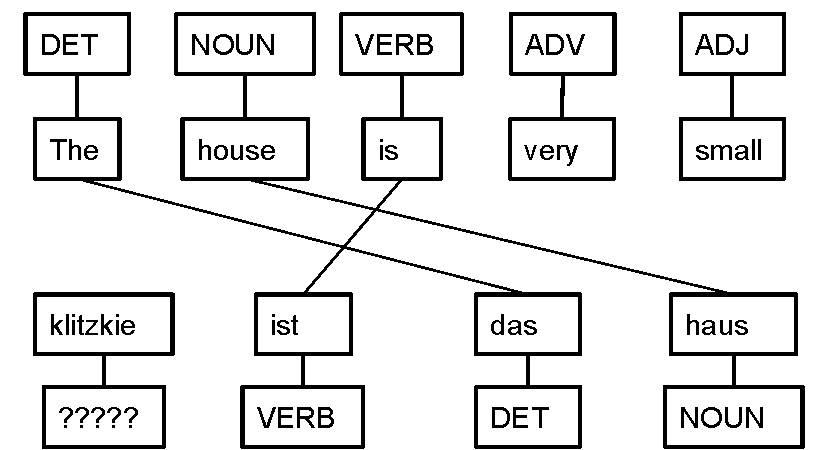
\includegraphics[scale=0.5]{Figures/LabelProjection}
\caption[Part-of-speech projection examples]{Examples of part-of-speech projection from English to German using parallel text. No tag is given to the German word \textit{klitzkie} that is not aligned.}
\label{fig:projection_example_en_de}
\end{figure}
Figure~\ref{fig:projection_example_en_de} shows an example of part-of-speech annotation projection from English to German through alignments. 
There are several successful application of this approach to low-resource part-of-speech tagging and noun-phrase chunking~\cite{YarowskyAndNgai}, dependency parsing~\cite{Hwa:2005:BPV}, named entity recognition~\cite{wang-che-manning:2013:ACL2013}.
The challenge to this approach is that (1) the alignment is not always accurate, (2) not all 
tokens in the target language got the annotation (e.g. German word \textit{klitzkie}) and (3) 
the projected annotation is not always linguistically correct in the target language. For 
example, in Malagasy all number are considered \textit{ADJ} (adjective) which is wrongly assigned as \textit{NUM} (number) if projected from English. 
This is the reason why the projected annotation is usually post-processed, mostly rule based ~\cite{Hwa:2005:BPV} or converted to soft-constrains~\cite{Das:2011,TackstromDPMN13} before feeding to the machine learning algorithm. 
\subsubsection{Model transfer}
% Why model transfer (accumulation of errors) ... 
The pipeline for annotation transfer is normally involve (1) the supervised model is trained on the source resource rich language, (2) use this model to provide annotation 
for the source language from bilingual data (3) project the annotation to the target language 
(4) use this projected annotation for target language model. Each step might introduce some 
noise, consequently the final target language model might be very biased. Therefore, instead 
of transferring the annotation, we can also transfer the model directly from the source 
resource rich languages to the target resource poor language~\cite{Zeman08cross-languageparser,P14-1126}. This is also the approach we took for many published work from this thesis including \emnlpiv, \emnlpv, \aclv\ and \conllv.  

% How can we do model transfer 
The model can only be transferred when both source and target features are in the same space. 
That is why the features that can be shared in both languages are desirable. Universal part-of-
speech tagset~\cite{UniversalTagSet} is an attempt to map any language specific tagset to the 
same universal tagset. Universal dependency treebank~\cite{11234/1-1699} is another attempt to 
map the annotation from different treebank to the same universal annotation. World Atlas of 
Language Structures~\cite{wals} which indicate structural properties of languages such as 
English has SVO structure or Japanese has SOV, can also be shared across 
languages.~\namecite{Naseem:2012:SSM} and~\namecite{tackstrom:2013:NAACL-HLT} use these 
features for transfering dependency parser.~\namecite{Tackstrom:2012:CWC} induced crosslingual 
word cluster where lexical items in both languages are grouped together using parallel data, also applied for transferring dependency parser. In this thesis, we 
investigate on crosslingual word embeddings where lexicon in several languages are represented 
as dense vector in the same semantic space, enable transfer learning. The crosslingual word 
embeddings must capture well the monolingual and bilingual relations in the semantic and 
syntactic space. We have successfully built and apply crosslingual word embeddings for several 
tasks in our \emnlpvi\ and \eaclvii\ \tofix{remove if not accepted} papers. 

% How to improve the performance of model transfer 
The transferred model from the source language is normally inadequate for the target language and usually need refinement~\cite{Zeman08cross-languageparser}.~\namecite{P14-1126} added the constrains from parallel data to the transfered model.~\namecite{McDonald:2011:MTD} additionally exploit multiple source languages. We, on the other hand, take advantage of a small annotated corpora. We show that we can correct much of the transferred model with the guideline from small annotated data.  
\begin{table}
\centering
\resizebox{\columnwidth}{!}{
\begin{tabular}{lm{5cm}m{6cm}}
\toprule
Paper & Topic & Resource  \\
\midrule
\namecite{kamper-etalInterspeech2015}      &  speech lexicon discovery  &  unlabelled speech \\
\namecite{Kamper:2016:UWS:2992449.2992455} & speech lexicon discovery & unlabelled speech \\ 
\namecite{Besacier:2014:ASR:2533333.2533656} & speech recognition & speech + transcription \\ 
\namecite{Khanagha:2014:PSS:2844738.2844801} & speech segmentation & unlabelled speech \\  
\midrule
\namecite{Gelling:2012:PCG:2390426.2390437} & dependency parsing and POS tagging & monolingual corpus\\
\namecite{sun-mielens-baldridge:2014:EMNLP2014} & dependency parsing &  small annotated corpus \\
\namecite{xia-lewis:2007:main} & dependency parsing & interlinear grossed text \\
\namecite{georgi-xia-lewis:2013:Short} & dependency parsing & small annotated corpus + interlinear grossed text \\
\namecite{Zeman08cross-languageparser} & dependency parsing & source language annotation \\
\namecite{tackstrom:2013:NAACL-HLT} & dependency parsing & source language annotations \\ 
\namecite{zhang-barzilay:2015:EMNLP} & dependency parsing &  source language annotation\\ 
\namecite{Naseem:2012:SSM} & dependency parsing &  source language annotation \\ 
\namecite{McDonald:2011:MTD} & dependency parsing & parallel corpus \\
\namecite{Ganchev:2009:DGI:1687878.1687931} & dependency parsing & parallel corpus \\ 
\namecite{Hwa:2005:BPV} & dependency parsing & parallel corpus \\ 
\namecite{P14-1126} & dependency parsing & parallel corpus \\ 
\midrule
\namecite{YarowskyAndNgai} & POS tagging & parallel corpus \\ 
\namecite{Duongacl13} & POS tagging & parallel corpus \\ 
\namecite{Das:2011} & POS tagging & parallel corpus \\ 
\namecite{TackstromDPMN13} & POS tagging & parallel corpus + POS dictionary\\ 
\namecite{Li:2012} & POS tagging & POS dictionary \\
\namecite{garrette:naacl13} & POS tagging & 2 hour annotation \\ 
\midrule
\namecite{DBLP:journals/corr/WangM13b} & Named Entity Recognition & parallel corpus \\ 
\namecite{darwish:2013:ACL2013} & Named Entity Recognition & parallel corpus + Wikipedia links  \\ 
\namecite{Nothman:2013:LMN:2405838.2405915} & Named Entity Recognition & Wikipedia links \\ 
\namecite{TsaiMaRo16} & Named Entity Recognition & Wikipedia links \\
\bottomrule
\end{tabular}
}
\caption{Notable related work on low-resource natural language processing.}
\label{tab:example_previous_work}
\end{table}

\subsection{Notable work}
Table~\ref{tab:example_previous_work} list notable published work on low-resource natural language processing covering some tasks related to speech, part-of-speech tagging, dependency parsing and named entity recognition with the data assumption. This is by no mean an exhaustive list but give some idea of what people have done for low-resource natural language processing and their resource assumption.  Some prior work use cheap resource such as monolingual data or unlabelled speech. However, many of them exploit parallel corpus which is harder to get for many low-resource languages, limiting their applicability. Most of the paper listed in Table~\ref{tab:example_previous_work} will be covered in more detail in subsequent sections. 


\section{POS tagging}
We will work with four main NLP tasks for low-resource languages in our thesis. They are POS tagging, dependency parsing, crosslingual word embedding and unwritten language processing. In this section we focus on the first task -- POS tagging which is the task of 
assigning morphological categories i.e. \textit{Noun}, \textit{Verb}, \textit{Adjective} etc to the lexical items. Moreover, POS tagging in useful in itself as an 
important step in many NLP pipelines, informing deeper layers of annotation, helping to understand the syntactic aspect of the language. We now briefly review prior 
approaches proposed for POS tagging for resource-poor languages, focusing on their supervision requirements. In our \emnlpiv\ paper, we present our own semi-
supervised learning approach which we argue has more realistic data requirements befitting the resource-poor scenario. 
%\subsection{Supervised learning} 
\subsubsection{Supervised Learning}
%\begin{figure}
%\centering
%\includegraphics[scale=0.6]{Figures/learningCurveSup}
%\caption{Learning curve for 3 languages: Dutch, Italian, and Swedish. Tagging accuracy is reported for the TNT tagger evaluated on the CoNLL shared task data, as described in Section~\ref{sec:annotatedData}.}
%\label{fig:lcSup}
%\end{figure}

The traditional approach to POS tagging builds a separate tagger for each target language, usually based on supervised machine learning algorithms~\cite{TNTTagger,Brill95transformation,Toutanova:2003}. %For each language they collate a large amount of manually annotated data for training a supervised POS tagger. %The supervised style for the traditional approach has achieved very high tagging accuracy, reaching as high as 95\% accuracy for many languages \cite{UniversalTagSet}. 
%The main challenge for POS tagging lies in the lack of training data. 
Supervised learning needs manually annotated data which is time consuming and costly to construct. If we were to apply supervised learning to a resource-poor language 
%TODO: put the table listing some state-of-the-art POS tagger.
the first question we have to consider is the amount of annotated data needed. This is a hard question to answer in general, due to the lexical and syntactic properties of the language, %it's common knowledge that it is usually harder to learn POS tagger for morphology rich language which denoted in bigger tagset size, 
 as well as the cost of manual annotation. 
% CPC How does the cost of annotation affect this?
%Figure~\ref{fig:lcSup} shows the learning curve for 3 languages, illustrating relatively high accuracy when trained on a corpus of 50k tokens, however accuracy diminishes for smaller training samples, for example, 1k tokens results in an absolute drop of roughly 20 percent.
%It's common knowledge that it is usually harder to learn POS tagger for morphology rich language which denoted in bigger tagset size. %The annotated data is from CoNLL shared tasks on dependency parsing~\cite{buchholz-marsi-2006}. 
%We use TNT tagger~\citep{TNTTagger} which is an implementation of second-order Hidden Markov Model. We use TNT because of its speed and close to the state-of-the-art performance. 
%Dutch, Italian and Swedish have 12, 30 and 41 tags respectively. At 50k tokens, Dutch achieves best performance, continue by Italian and Swedish. This confirm our intuition that bigger tagset are usually harder to learn. 

%POS tagging information are usually used within other applications. Each context yields a different performance requirement. For example, dependency parsing directly use POS information. A single POS error might lead to fail dependency parsing tree. Thus, we might need %POS tagging accuracy as high as 95\% or 97\% requiring 
%much more than just 50k tokens. %On the other hand, other tasks such as noun-phrase chunking is less severely affected by POS tagging accuracy. In that case, probably $\sim$90\% accuracy which requires around 30k annotated tokens to train on, is acceptable. 
Moreover, corpus annotation is time consuming and costly. For example, for the POS layer of the Penn Treebank~\cite{PenTreeBank} it took 3 years to annotate 4.5 million tokens. We cannot expect anywhere near as a large annotated corpora for resource-poor languages. However, \namecite{garrette:acl13} show that POS annotations for 1,000 tokens are easy to acquire with around 1 hour of manual effort. This raises the challenge of how we can best make use of such tiny amounts of annotated data. %Naively using supervised learning on this sized data results in low accuracy, as illustrated in Figure~\ref{fig:lcSup}, and in this paper we developing approaches to improve accuracy by combine this form of limited supervision with an unsupervised projection approach. 
%Moreover, figure~\ref{fig:lcSup} also shows that Italian and Swedish POS performance are actually converging. Adding more data are not likely to boost the performance. We should find another source of information aside from supervised data to aid the learning process. This will be discussed in more detail in Section~\ref{sec:semisup}. 


\subsubsection{Unsupervised learning}
Unsupervised approach is typically suitable for resource-poor language since it doesn't need any manually annotated data and unlabelled data is relatively easy to acquire. These approaches try to group words having the same morphological/syntactic properties into the same group (cluster)~\cite{Christodoulopoulos:2010,unSupPOSClustering,chineseWhisper}. It is believed that words in the same cluster are likely to have the same POS tag. One problem with this approach is determining the number of clusters. Defining that number beforehand might not be a good solution~\cite{unSupPOSClustering}. We might force the algorithm to separate coherent clusters or to join unrelated ones. On the other hand, letting the algorithm choose when to stop could result in a too specific or too general clusters. Evaluation is also another major consideration, since we don't have the gold data to compare with. %Evaluation is also another major consideration. Normally, clustering algorithms are evaluated based on the perplexity (or entropy) of the cluster~\citep{Christodoulopoulos:2010}. In the case of tagging, we are expecting that all words in the same cluster have the same tag. Therefore, the lower the perplexity, the better. However, is it what we are looking for? The answer is no, we want to compare with gold-standard test data to know the tagging performance. \citep{ManyToOneEvaluate} suggested a \textit{many-to-one} evaluation. The induced tag for each cluster is the most frequent tag of the items in the cluster, consulting the gold-standard data. However, there can be cases where two clusters have the same tag. To resolve this issue,\textit{ one-to-one} evaluation puts the restriction that each gold tag corresponds to one cluster only. Normally, this is done by greedy matching, which aims at maximizing  accuracy. Nevertheless, the number of clusters and gold tags are likely to be different. In that case, some clusters or gold tags will not be matched. However, both \textit{many-to-one} and \textit{one-to-one} evaluation schemes require gold-standard data to find the most appropriate tag for each cluster. This is a chicken-and-egg problem since if we have gold-standard data then we do not need to take an unsupervised approach. Besides, we can also use some heuristic method to determine the tag for each cluster such as cluster size (e.g. the biggest cluster is Noun). 
%Unsupervised approach is typically suitable for resource-poor language since it doesn't need any manually annotated data and unlabelled data is relatively easy to acquire. 
However, the biggest problems introduced by unsupervised approach is the poor performance~\cite{Christodoulopoulos:2010,Blunsom:2011} hinder its usage in real world applications. %Some unsupervised POS tagger might still achieve quite high performance  using tag dictionary \cite{Goldberg08emcan,Das:2011}. However, tag dictionary is also a huge form of supervision and very expensive to acquire. 

\subsubsection{Semi-supervised learning}
As mentioned above, supervised learning needs large training corpora, 
which are only available for resource-rich languages. Unsupervised POS tagging, on the other hand, is suitable for resource-poor languages since requires only unannotated text, however their relatively poor performance is not suitable for practical applications. 
Semi-supervised learning appears to better fit which is also the approach in our \emnlpiv\ paper. We show that we can achieve high performance POS tagger exploiting only tiny amount of annotated data and some distance supervision from additional resources. It is important to understand what kind of supervision signal we might have from additional resources which will be reviewed in the following.
%However, to further improve the performance, we also incorporate different 
%It is desirable to find a different form of supervision to compensate for the lack of annotated data which will be reviewed below. 
%---------------------
\subsection{Typologically related information}

For closely related languages, such dialects of the same language or those in the same language family, the lexicon and syntactic structures of the languages are likely to be highly similar. These kinds of similarities can be exploited when developing tagging models for low-resource languages \cite{Hana04,Feldman06,reddy2011crosspos}. They propose tying together the transition probabilities and estimating the emission probability separately either by mimicking the source language lexicon or with supervised learning from a small amount of annotated data. Note that this method does not need parallel data, as no alignments are required, however monolingual annotated data is required for related languages, which is unlikely to be available for many low-resource languages.\footnote{Especially for languages only spoken by small communities, in which case the best we might hope for is parallel data between the target language and a mainstream `contact' language, such as English or a pidgin.}  

\subsection{Projected information}

\namecite{YarowskyAndNgai} pioneered the use of parallel data for projecting tag information from a resource-rich language to a resource-poor language. They first tag the source resource-rich language using a supervised POS tagger, and the tagging is then projected to the target resource-poor language through a word alignment. They observed that although this works well in many cases, the projected tags are very noisy. Thus, they apply a heuristic based on sentence alignment score to filter out noisy alignments. Finally, the projected tags are used to build the target language tagger, which can then be applied to other texts. \namecite{Duongacl13} used a similar method on using sentence alignment scores to rank the goodness of sentences. They trained a seed model from a small part of the projected data, then applied this model to the rest of the data using self-training with revision.

%SB: the following paragraph is hard to follow
\namecite{Das:2011} also used parallel data but additionally exploited graph-based label propagation to expand the coverage of labelled tokens. Each node in the graph represents a trigram in the target language. Each edge connects two nodes which have similar context. Originally, only some nodes received a label from direct label projection, and then labels were propagated to the rest of the graph. Rather than use the labels directly, \namecite{Das:2011} instead use the labels to extract a tag dictionary which is used as constraints in learning a feature-based HMM \cite{featurebaseHMM}. Both \namecite{Duongacl13} and \namecite{Das:2011} achieved 83.4\% accuracy on the test set of 8 European languages (Table~\ref{tab:taggingAccPrevModels}).

\begin{table*}
\tabcolsep 3pt
\begin{center}
\begin{tabular}{lccccccccc|c}
\toprule
        ~ & da & nl & de & el & it & pt & es & sv & & Average \\
\midrule
\namecite{Duongacl13} & 85.6 & 84.0 & 85.4 & 80.4 & 81.4 & 86.3 & 83.3 & 81.0 & & 83.4 \\      
\namecite{Das:2011} & 83.2 & 79.5 & 82.8 & 82.5 & 86.8 & 87.9 & 84.2 & 80.5 & & 83.4 \\
\namecite{Li:2012} & 83.3 & 86.3 & 85.4 & 79.2 & 86.5 & 84.5 & 86.4 & 86.1 & & 84.8 \\
\namecite{TackstromDPMN13} & 88.2 & 85.9 & 90.5 & 89.5 & 89.3 & 91.0 & 87.1 & 88.9 & & 88.8 \\
\bottomrule
\end{tabular}
\caption[Previously published token-level POS tagging accuracy]{Previously published token-level POS tagging accuracy for various models across 8 languages: Danish (da), Dutch (nl), German (ge), Greek (el), Italian (it), Portuguese (pt), Spanish (es), Swedish (sv) evaluated on CoNLL data.% as described in Section~\ref{sec:annotatedData}. %~\cite{buchholz-marsi-2006}.%The best results on each language, and on average, are shown in bold
 }
\label{tab:taggingAccPrevModels}%
\end{center}
\end{table*}

\subsection{Dictionary Information}
A tag dictionary specifies the set of allowable tags for a word. Even an incomplete or noisy tag dictionary is sufficient to allow for a POS tagger to be learned using standard unsupervised inference, such as the Expectation Maximization (EM) algorithm, where the entries in the tag dictionary are used to constrain the tags for each word~\cite{Kupiec1992225,Merialdo:1994,Banko:2004,Goldberg08emcan}. The usefulness of tag dictionaries is due to many words having very few possible tags and thus the tag dictionary drastically restricts the search space, while also steering EM away from poor local optima.
%% LONGDT : Need to put the citation here. I remember reading somewhere said that 90% of the words in French corpus have less than 2 possible tags.
With a dictionary derived from gold-standard data \namecite{Das:2011} achieved an accuracy of approximately 94\% on the same 8 languages. The effectiveness of a gold-standard dictionary is undeniable, however it is costly to build one, especially for resource-poor languages. Cheaper crowd-sourced dictionaries are also valuable, as demonstrated by \namecite{Li:2012} used Wiktionary\footnote{wiktionary.org} to achieve 84.8\% accuracy on the same 8 languages (see Table~\ref{tab:taggingAccPrevModels}). Note, however, that there are large differences in the performance for words appearing in dictionary and out-of-vocabulary (OOV) words (89\% vs 63\%), which suggests that their approach will be of much less use for small and incomplete POS dictionaries. 

\namecite{TackstromDPMN13} combined both token information from bilingual projection and type 
constraints from Wiktionary to achieve the current state-of-the-art in low-resource tagging. 
Their approach first builds a tag lattice, which is then pruned using the token information 
and type constraints. The remaining paths are used to train a Conditional Random Field (CRF) 
tagger. They achieved 88.8\% accuracy on the same 8 languages (see 
Table~\ref{tab:taggingAccPrevModels}). In our \emnlpiv\ paper, we will mainly compare the 
results of our approach with~\namecite{TackstromDPMN13}. Note that our method and theirs have 
very different data requirements: we use a small corpus of annotated part-of-speech in the 
target language, but only limited parallel data and no tag dictionaries, while they use orders 
of magnitude more parallel data as well as implicit supervision courtesy of their tag 
dictionary. As argued above, while both approaches have limited supervision, our data 
requirements are more appropriate to a low-resource scenario. 

Table \ref{tab:taggingAccPrevModels} summarises the performance of the above models across all 8 languages. Note that these methods vary in their reliance on external resources. The systems listed in Table~\ref{tab:taggingAccPrevModels} are sorted in the ascending order of resource usage.~\namecite{Duongacl13} use the least, i.e.\ only the Europarl Corpus~\cite{europarl}.~\namecite{Das:2011} additionally use the United Nation Parallel Corpus.~\namecite{Li:2012} did not use any parallel text but used Wiktionary.~\namecite{TackstromDPMN13} exploited most parallel data by additionally using parallel data crawled from web, as well as 
%\fixme{We don't have the specific statistic of how much they use}
using the tag dictionary from~\namecite{Li:2012}. The pattern of results in Table~\ref{tab:taggingAccPrevModels} illustrates the common lesson in NLP: when adding additional resources, the models perform better.  
 
\subsection{Small Annotated Data Information}

An alternative approach for tagging resource-poor languages is to assume a small corpus of manually annotated data. \namecite{garrette:acl13} built a POS tagger for two resource-poor languages, Kinyarwanda (\texttt{Kin}) and Malagasy (\texttt{Mlg}). They used no parallel data, but instead exploited four hours of manual annotation to label 4,000 tokens or 3,000 word-types. These tokens or word-types were used to build a tag dictionary. They employed label propagation to expand the coverage of this dictionary, much like \namecite{Das:2011}. The dictionary was used to label training examples, from which they learned a tagger. This achieved 81.9\% and 81.2\% accuracy for \texttt{Kin} and \texttt{Mlg} respectively. %Note that although they claim to use only 4 hours of annotation, their use of an external tag dictionary compromises this claim, and consequently limits the portability of their approach to other low-resource settings which do not have existing dictionaries.
 
The method we propose in our \emnlpiv\ paper is similar in that we also use a small amount of annotation. However, we directly use the annotated data to train the model rather than indirectly via a tag dictionary. We argue that with a proper ``guide'', namely parallel projection, we can take advantage of very limited annotated data. Furthermore, our approach is also able to use a dictionary, although even without this form of supervision our method results in high accuracy taggers, well above baseline approaches and in most cases outperforming the previous state-of-the-art.  
% tac -- I added the last sentence. Feel free to cut if you this it's too much.
% LDC -- I think it's fine 
%---------------------
 
% This should be the conclusion for this chapter 
%In our EMNLP 2014 paper, we propose a semi-supervised method to narrow the gap between supervised and unsupervised 
% approaches. We demonstrate that even a small amount of supervised data leads to substantial improvement. 
% Aside from this small amount of annotated data, the supervision signal also comes from parallel data of 
% the resource-rich (source) and resource-poor (target) languages. The parallel data provides a 
% bridge that enables us to transfer POS information from a resource-rich to a resource-poor language through the word alignment. 

%While annotated text tends to be expensive to acquire, parallel data between the resource-rich and resource-poor languages, on the other hand, is relatively easier to acquire in many cases, thanks to the development of multilingual documents from government projects, book translations, multilingual websites, and so forth. Moreover, this approach also exploits the idea that tag ambiguity in one language is disambiguated through different alignments. Consider the example, \textit{Buffalo buffalo buffalo buffalo},\footnote{The bison of Buffalo (a city in the United States) bully (other) bison.} and its Vietnamese translation \textit{Trau o Buffalo bat nat trau khac}, as in Figure \ref{fig:EnViparallel}. The ambiguous usages of \textit{buffalo} have different translations: \textit{trau} (common noun - \textit{NNS}), \textit{bat nat} (verb - \textit{VB}), \textit{Buffalo} (proper noun - \textit{NNP}). Thus, the different translations help to disambiguate the POS tag of the word \textit{buffalo}.
%\begin{figure}
%\centering
%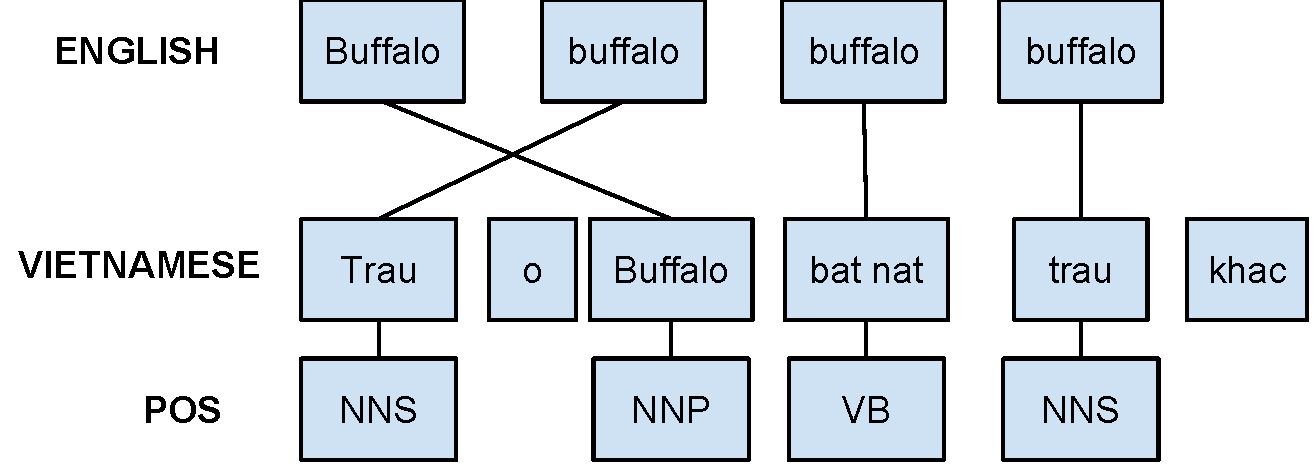
\includegraphics[scale=0.5]{Figures/Buffalo_buffalo}
%\caption{Sample of English--Vietnamese parallel data. The usages of the ambiguous English word \emph{buffalo} are disambiguated through their alignment with different Vietnamese words.}
%\label{fig:EnViparallel}
%\end{figure}

%\section{Background and Related Work}
%\label{sec:semisup}
%As mentioned above, semi-supervised or distantly-supervised methods are well suited to resource-poor languages. In this section, we review forms of supervision used in semi-supervised methods for low-resource POS tagging in the literature. 
% PRT shouldn't be include in the Universal tagset
\begin{table}[t]
\centering
\tabcolsep 3pt
\begin{tabular}{crcl}
\toprule
Lang & Size (k) & \# Tags & Not Matched \\
\midrule
da & 94 & 8 & DET, PRT, PUNC, NUM \\
nl & 203 & 11 & PRT \\
de & 712 & 12 & \\
el & 70 & 12 & \\
it & 76 & 11 & PRT \\
pt & 207 & 11 & PRT \\
es & 89 & 11 & PRT \\
sv & 191 & 11 & DET \\
\midrule
kin & 9.3 & 9 & PRT, PRON, NUM\\
mlg & 9.5 & 11 & NUM \\
\bottomrule
\end{tabular}
\caption[The size of annotated data, number of tags included and missing for all considered languages]{The size of annotated data, number of tags included and missing for the 8 European languages: Danish (da), Dutch (nl), German (de), Greek (el), Italian (it), Portuguese (pt), Spanish (es) Swedish (sv) and 2 resource-poor languages Kinyarwanda (\texttt{Kin}) and Malagasy (\texttt{Mlg}).} 
\label{tab:tagMissing}
\end{table}

\subsection{Universal tagset}
\label{sec:universalTagset}
Core to many of the projection methods described above is an assumption of a matching tagset between the source and target languages. That way the labels projected from the source have meaning in the target language, and can be used directly as target labels, constraints, etc. It is uncommon for languages to have been annotated with same tag set, for this reason these approaches use the universal POS tagset~\cite{UniversalTagSet}. This tagset consists of a list of tags that are said to be shared across languages, as well as mappings into this scheme from native tagsets in several languages. The universal tagset is extremely useful in multilingual applications, enabling joint multi-lingual modelling as well as simpler evaluation of results across languages. 
In our setting, using the universal tagset can simplify our problem, removing the difficult issue of matching between different tagsets. 
For low-resource languages without an official tagset, such as Bengali or Lahnda, the universal tagset would be a good starting point for linguistic annotation.

The universal tagset from~\namecite{UniversalTagSet} consists of 12 common tags: \textit{NOUN, VERB, ADJ} (adjective), \textit{ADV} (adverb), \textit{PRON} (pronoun), \textit{DET} (determiner and article), \textit{ADP} (preposition and post-position), \textit{NUM} (numerical), \textit{CONJ} (conjunctions), \textit{PRT} (particle), \textit{PUNC} (punctuation) and \textit{X} (all other categories including foreign words and abbreviations). \namecite{UniversalTagSet} provide the mapping from several language-specific tagsets to the universal tagset.

Nevertheless, using universal tagset looses information, such as tense and case information is often lost in the mapping. For example, the Penn treebank tags verbal tags \textit{VB, VBD, VBG, VBN, VBP, VBZ} are mapped to the generic \textit{VERB} tag in the Universal tagset. Moreover, the mapping is not always straightforward. Table \ref{tab:tagMissing} shows the size of the annotated data for each language, the number of tags presented in the data, and the list of tags that are not matched. We can see that only 8 tags are presented in the annotated data for Danish, i.e, 4 tags (\textit{DET, PRT, PUNC,} and \textit{NUM}) are missing.\footnote{Many of these are mistakes in the mapping, however, they are indicative of the kinds of issues expected in low-resource languages.}
%LongDT : why it's missing, because of mapping or linguistic reason? Could you check this for me Steven ?
%Therefore, when we project the labels from a resource-rich language (i.e, English) to Danish through alignment, we won't get any credit from tokens tags as either \textit{DET, PRT, PUNC} or \textit{NUM}.
Thus, a classifier using all 12 tags will be heavily penalized in the evaluation.

\namecite{Li:2012} considered this problem and tried to manually modify the Danish mappings i.e. map tag \textit{AC} and \textit{AO} as \textit{NUM} or match tag \textit{U} to \textit{PRT} etc. Moreover, \textit{PRT} is not really a universal tag since it only appears in 3 out of the 8 languages.~\namecite{plank-hovy-sogaard} state that \textit{PRT} often gets confused with \textit{ADP} even in English. We will later show that the mapping problem causes substantial degradation in the performance of a POS tagger exploiting parallel data. The method we present in our \emnlpiv\ paper is more target-language oriented: our model is trained on the target language, in this way, only relevant information from the source language is retained. Thus, we automatically correct the mapping, and other incompatibilities arising from incorrect alignments and syntactic divergence between the source and target languages. 
 
\section{Dependency Parsing}

\begin{figure}
\centering
\begin{minipage}{.5\textwidth}
  \centering
\Tree [.S [.NP [.PRP I ] ].NP [.VP [.VBP like ] [.NP [.DT a ] [.JJ big ] [.NN meal ] ].NP ].VP ].S
\end{minipage}%
\begin{minipage}{.5\textwidth}
  \centering
\begin{dependency}[theme = simple]
   \begin{deptext}[column sep=1em]
      I \& like \& a \& big \& meal \\
   \end{deptext}
   \deproot{2}{ROOT}
   \depedge{2}{1}{NSUBJ}
   \depedge[arc angle=90]{2}{5}{DOBJ}
   \depedge[edge start x offset=0pt, arc angle=80]{5}{3}{DET}
   \depedge[edge start x offset=-7pt, arc angle=30]{5}{4}{AMOD}
\end{dependency}
\end{minipage}
\caption{Phrase structure tree (Left) and Dependency tree (Right) of the same sentence.}
\label{fig:parseSample}

\end{figure}


%%% VIETNAMESE EXAMPLES 

%\begin{dependency}[theme = simple]
%   \begin{deptext}[column sep=1em]
%      Manh \& dat \& cua \& dan \& bom \& khong \& con \& nguoi \& ngheo \\
%   \end{deptext}
%   \deproot{7}{ROOT}
%   \depedge{7}{1}{NSUBJ}
%   \depedge[edge start x offset=-7pt, arc angle=90]{7}{6}{NEG}
%   \depedge[edge start x offset=7pt, arc angle=80]{1}{2}{AMOD}
%   \depedge{1}{3}{DET}
%   \depedge{3}{4}{POBJ}
%   \depedge{4}{5}{NN}
%   \depedge{7}{8}{DOBJ}
%   \depedge{8}{9}{AMOD}
%   \depedge[edge start x offset=0pt, arc angle=80]{7}{3}{DET}
%   \depedge[edge start x offset=-7pt, arc angle=30]{5}{4}{AMOD}
%\end{dependency}


%\begin{figure}
%\centering
%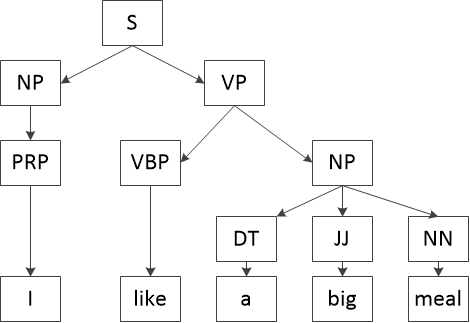
\includegraphics[scale=0.5]{Figures/phraseStructure}
%\;\;\;\;\;\;
%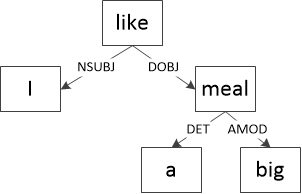
\includegraphics[scale=0.6]{Figures/dependencyParse}
%\caption{Phrase structure tree (Left) and Dependency tree (Right) of the same sentence}
%\label{fig:parseSample}
%\end{figure}
While part-of-speech tagging  operates in the word level, provides information about syntactic category of each separate word in the sentence, we move to the sentence level in the second task which is parsing. Sentence parsing is the task of understanding the underlying structure of sentence. There are two main structure representations: (1)~phrase structure tree (2)~dependency tree. Phrase-structure tree represents nesting structure of phrases such as noun phrase, verb phrase, preposition phrase etc. Dependency tree, on the other hand, shows the dependencies between words. For example, the sentence ``\textit{I like a big meal}" has two representations as shown in Figure \ref{fig:parseSample}.

Phrase structure tree is more meaningful for understanding grammatical (syntactic) structure of the sentence. However, for each language, the phrase structure might be very different. For example, English favours \textit{``Subject Verb Object"} structure while Japanese switch the position of \textit{Object} and \textit{Verb} (always puts \textit{Verb} at the end of the sentence). Thus, when copying information from the source language to the target language, phrase structure tree is not particularly suitable. Dependency tree, in contrast, shows the semantic structure i.e. answering question such as \textit{who did what to whom by which means?}. Thus, dependency structure will be more transparent across languages. In addition, dependency tree are better at capturing long distance relations which is desirable in many applications.  
%Todo : list of advantages of dependency structure 
We are going to use this structure for building parser for target resource-poor languages.

Dependency tree is usually formalized as labelled directed graph G = (V,A) where V is the set of nodes, A is the set of arcs. For example, the dependency tree in Figure~\ref{fig:parseSample} has 
\begin{align}
V &= \{I, like, a, big, meal\}\\
A &= \{(like, nsubj, I), (like, dobj, meal), (meal, det, a), (meal, amod, big)\} 
\end{align}
$A$ is the set of $(w_i,r,w_j)$ which represent the relation $r$ from the head $w_i$ to dependent $w_j$.%~\namecite{Kubler:2009:DP:1538443} suggested some relations between head and dependent: 
%\begin{itemize}
%\item  $w_i$ is compulsory but $w_j$ is optional 
%\item $w_i$ select $w_j$ and determine the roles of $w_j$ whether obligatory or optional
%\item  The form of $w_j$ depends on $w_i$ with respect to agreement and government. 
%\item The linear position of $w_j$ is determined according to $w_i$
%\end{itemize}
Most of the time the roles of head and dependence are very distinguishable. However, sometime it is hard to distinguish, especially when it involves articles, complementizers and auxiliary verbs etc. For example, in the sentence \textit{I give up my thesis}, it's unclear whether $give$ is the head of $up$ or vice versa. Due to all these uncertainty, dependency parsing is a much harder task compared with POS tagging especially in the low-resource scenario. 
The rest of this section is organized as follow. In section~\ref{sec:monolingualDep}, we are going to review some supervised methods to build a dependency parser. In section~\ref{sec:crosslingualDepParsing}, we reviewed crosslingual methods applied to resource-poor languages. 

\subsection{Supervised dependency parsing}
\label{sec:monolingualDep}
\subsubsection{Grammar-based approach}
Phrase structure tree has a long history. Many algorithms are developed to parse phrase structure tree. Naturally, people want to apply the phrase structure approaches to dependency parsing. One of the notable approach is using context free dependency grammar in similar vein to context free grammar of phrase structure parsing. However, in context free dependency grammar, all non-terminal nodes (e.g. \textit{S, NP, VP}) are replaced with an actual word. This is the simplest way to convert from phrase structure grammar to dependency grammar.~\namecite{Nivre_twomodels,eisner-blatz-2007,MarkP07-1022} proposed more complicated but also more efficient method for conversion. After the dependency grammar is constructed, we can directly use any phrase structure parsing algorithm such as CKY~\cite{Younger1967189}. One disadvantage of using dependency grammar is that it's very hard to capture long distance relations or apply to non-projective parsing.  

Another adaptation for dependency parsing use the tree conversion rules. That is, the sentence is parsed using phrase structure. Phrases are converted to dependency relation using head-rules~\cite{Marneffe06generatingtyped,Yamada03statisticaldependency}. However, these rules are language specific and normally need a lot of expertise to build. 

\subsubsection{Transition-based approach}
Transition based parsing is more recently developed~\cite{Nivre:2008:ADI}. It is similar to finite state automaton which consists of set of \textit{configurations} and \textit{transitions}. The parsing algorithm will choose a list of transitions that transform the initial configuration to the terminal configuration. 
\paragraph{Configuration}
Given a sentence $w = w_0,w_1, ... w_n$, with $w_0$ is the dummy $ROOT$, a configuration is defined as a triple $c=(S,Q,A) $ where 
\begin{itemize}
\item $S$ is the stack of partially proceeded words. 
\item $Q$ is the queue of remaining words 
\item $A$ is the set of arcs that form partially parsed tree. 
\end{itemize}
Each configuration $c$ aims at capturing a partial analysis of a sentence. The initial configuration for the above sentence $w$ is defined as 
$$c_{init}  = (S_0,Q_0,A_0)$$ 
Where $S_0 = [w_0]$ contains only the dummy $ROOT$. $Q_0 = [w_1,w_2,...w_n]$ contains all the remaining words and $A_0 = [\texttt{Empty}]$. The terminal configuration is defined as 
$$c_{terminal} = (S_{ter}, Q_{ter}, A_{ter}) $$ 
Where $Q_{ter} = [\texttt{Empty}]$ for any $S_{ter}$ and $A_{ter}$. That is, the algorithm terminates when there isn't any word left needed to proceed in the queue regardless of $S_{ter}$ and $A_{ter}$. 
% To Do : Give an example here 

\paragraph{Transition}
The set of transitions are used to transform the initial configuration $c_{init}$ to the terminal configuration $c_{terminal}$. Basically, there are 3 transitions.
\begin{itemize}
\item \texttt{left-arc}($r$)\;\; : $(S|w_i,\; w_j|Q,\; A) => (S,\;w_j|Q,\; A\cup \{(w_j,r,w_i)\})$
\item \texttt{right-arc}$(r)$ : $(S|w_i,\; w_j|Q,\; A) => (S,\;w_i|Q,\; A\cup \{(w_i,r,w_j)\})$
\item \texttt{shift}$ \;\;\;\;\;\;\;\;\;\;\;\;\;\;\;\;\;\;: (S,\; w_i|Q,\; A) \;\;\;\;\;=> (S|w_i,\;Q,\; A)$
\end{itemize}

% Todo : Add the description for each transition 
The \texttt{left-arc}($r$) for dependency relation $r$ with $w_i$ at the top of stack $S$ and $w_j$ at the first position of queue $Q$, add a dependency arc $(w_j,r,w_i)$ to $A$ and pop the stack. Pre-condition for \texttt{left-arc} is that both stack and queue are non-empty and $i\neq0$. The \texttt{right-arc}($r$) for dependency relation $r$ adds the dependency $(w_i,r,w_j)$ to $A$ but pop the stack and replace the first element of queue with $w_i$. The precondition is both stack and queue are non-empty. \texttt{shift} simply remove the first word of queue and put at top of stack. The precondition is that buffer is non-empty. 

\paragraph{Parsing Algorithm}
The parsing algorithm decides what transition is applied to a given configuration.~\namecite{Nivre:2008:ADI} formalized it as a supervised classification task. The dependency treebank is converted to the training data using some heuristic rules.\footnote{This training data can be generated dynamically as in~\namecite{C12-1059}.} The classifier is trained on this data set. Crucially, the classifier should give confidence/ranking for each prediction.
Since if the first prediction is not applicable (i.e. the pre-condition is not satisfied), the second one will be considered etc. 
% To do: proof that algorithm always terminate. 
The algorithm always terminate in $O(n)$ steps. Each \texttt{left-arc} or \texttt{right-arc} reduces the stack size by 1 and \texttt{shift} increase the stack size by 1. There are maximum $n$ \texttt{shift} operation since each \texttt{shift} also reduces the queue size by 1. Therefore, maximum number of \texttt{left-arc} and \texttt{right-arc} is also $n$. Thus, maximum number of transitions is $2\times n$. Moreover, the parsing algorithm can always pick a valid transition for each configuration because \texttt{shift} is always a valid one (except if the current configuration is the terminal configuration). 
%Todo : talk more about feature set and algorithms 
% Todo : more accurate system can be achieve by not using static rules 
There are many variations of the transition based parsing. \namecite{Nivre:2009:NDP:1687878} introducing \texttt{swap} transition to deal with non-projective dependency parsing.~\namecite{chen-manning:2014:EMNLP2014} exploited neural network based classifier for the parsing algorithm instead of the original support vector machine classifier which we extended for our \aclv, \emnlpv, \conllv\ papers. 

\subsubsection{Graph-based approach }
The graph based approach formalizes dependency parsing task as finding the maximum spanning tree on the weighted fully connected graph~\cite{McDonald:2005:NDP}. The graph $G = (V,E)$ for a sentence $w = w_0,w_1,w_2....w_n$ is constructed as follow. 
\begin{itemize}
\item V = {$w_0,w_1,...w_n$}
\item E = {$(w_i,\text{weight},w_j)$} for every $i,j$
\end{itemize}
~\namecite{1264361} algorithm is used to find the maximum spanning tree. First, all vertexes are selected. Incoming edge with highest weight are added to the graph one by one. If the resulting graph is a tree then it's the maximum spanning tree. If it's not, the cycle is collapsed into a single node, the weights are updated and the algorithm is repeated. The remaining question is how to estimate the weight of each edge.~\namecite{McDonald:2005:NDP} applied the Margin Infused Relaxed Algorithm (MIRA) for estimating those weights on the treebank. 

Graph-based approach is the natural solution for non-projective dependency parsing since it makes no assumption on the word order. Unlike transition-based approach, graph-based is exact inference. Therefore, the running time is much slower. However, graph-based approach is more robust. Transition-based approach is prone to errors meaning that error in early state might accumulate and led to bias model. An interesting observation is that errors made by graph-based approach and transition-based approach is very different and mostly not overlapping.~\namecite{Nivre08integratinggraphbased,Zhang:2008:TTP} proposed method to combine the strength of both approach in a hybrid approach. 
%Todo : talk more about hybrid approach here 

%\subsection{ConLL shared task on dependency parsing}
%The ConLL 2006 and 2007 organized the shared task on dependency parsing for various languages. 
%\subsection{Evaluation}
\subsubsection{Evaluation}
The common evaluation metric for dependency parsing is attachment score which is the percentage of word having the correct head thanks to the single-head property of the dependency tree. There are two version of attachment score which are unlabelled attachment score (UAS) and labelled attachment score (LAS). The first one only look at head while the second metric additionally look at dependency labels. 
%- UAS vs LAS 
%- Total sentence score 
%- Ignore punctuation (Interesting story here). Use malt eval or official web.
%- Limit evaluation to 10 words or less 

\subsubsection{Universal Treebank}
Similar with universal POS tagset, it is highly desirable for universal annotation for 
dependency treebank.~\namecite{DBLP:conf/lrec/ZemanMPRSZH12} pioneer on building an unify 
annotation (HAMLED) for treebank in multiple languages. They propose the mapping to transform 
each language specific treebank to the Prague Dependency Treebank 
style~\cite{bohmovahhh:2001}. 
~\namecite{mcdonald-EtAl:2013:Short} took the different approach and built the Google 
universal treebank for many languages using the Stanford dependency 
style~\cite{deMarneffe:2008:STD:1608858.1608859} and the universal POS 
tagset~\cite{UniversalTagSet}.~\namecite{ROSA14.915} 
extended~\namecite{DBLP:conf/lrec/ZemanMPRSZH12} to build HAMLED 2.0 which covers more than 30 
languages using similar annotation with Google universal treebank. 
As an effort to better accommodate language differences and unify prior work, 
\namecite{11234/1-1699} proposed universal dependency treebank, employing the Stanford 
universal dependency annotation~\cite{DBLP:conf/lrec/MarneffeDSHGNM14} which currently is the 
largest collection of dependency treebank in more than 40 languages. 

\subsection{Low-resource Dependency Parsing}
\label{sec:crosslingualDepParsing}
Consistent dependency treebank annotation typically requires careful guideline design, guideline testing and refinement, annotator quality control etc. %For Prague Dependency Treebank (PDT), it took a year for the first 1000 sentences~\cite{bohmovahhh:2001}, most of the time-consuming part is the annotation guideline and quality control. % but the next 20000 sentences took only a year too~\cite{bohmovahhh:2001}. 
We can't expect this high quality resource available for a resource-poor language. In this section, we are going to review prior approaches to build a dependency parser to a target resource-poor language.
 
\subsubsection{Delexicalization approach}
This approach builds a delexicalized parser from a resource-rich source language where a treebank is available. The delexicalized parser is built simply by removing lexical features and then apply any standard supervised monolingual parser. This parser is then applied directly to the target resource-poor language. The underlying hypothesis is that aside from lexical items, other features are similar between two languages. 
Delexicalized parser is first proposed by~\namecite{Zeman08cross-languageparser}. They wanted to build parser for Swedish using Danish. Noted that the hypothesis hold true between Swedish and Danish since they are very similar languages.  They scored 66.4\% F1 labelled attachment score for Swedish. This is an encouraging result since they did not use any external resource such as bilingual dictionary or parallel data. 

\namecite{McDonald:2011:MTD} also exploit the idea of delexicalized parser. They experiment with 8 European languages. The main contribution of this paper stems from the incorporation of parallel data to the model. % Todo : can expand here, can include the predicted POS to the result 
\namecite{Sogaard:2011:DPS} is another example exploiting the delexicalized parser for a target language. Instead of choosing the source language that is similar to the target language, he investigates on choosing the data points from source language that are similar with the target language with respect to POS sequences.

So far, the delexicalized parser only uses POS information.~\namecite{tackstrom:2013:NAACL-HLT} extended the POS features to other cross-lingual features. They adopted the WALS -- World Atlas of Language Structures~\cite{wals} --  typological features in the similar vein with~\cite{Naseem:2012:SSM}. WALS covered basic information such as order of \textit{Subject}, \textit{Object}, \textit{Verb}; order of \textit{Adjective} and \textit{Noun}; order of \textit{Adposition} and \textit{Noun} etc.  about nearly 2700 languages. They experiment with 16 languages. For each target language, the rest 15 languages will be the training data. The intuition here is very simple. They want to take advantage of multiple source-languages. Moreover, they also apply self-training and ensemble-training for relexicalized the delexicalized model. 

\subsubsection{Projection approach}
In contrast to the approach using language relatedness clues, i.e. delexicalized parser. In this section, we are going to investigate on the method exploiting parallel data to either project the annotation from the source to the target language or as the constrains for a better model. 

\namecite{Hwa:2005:BPV} is the first to exploit this idea. The key assumption of this paper is the direct correspondence hypothesis between parallel text. Using this assumption, they define a set of actions for each of the one-to-one, one-to-many, many-to-one, one-to-null or many-to-many alignment. Given a source-language parsed tree and the word alignment, they apply a series of defined actions to generate the target-language parsed tree. However, the performance of this direct transfer is quite poor. They resolve this by applying a set of post-processing rules which capture the language specific knowledge. They achieved 72.1 and 53.9\% UAS for Spanish and Chinese respectively. However The approach of~\namecite{Hwa:2005:BPV} contains many heuristics and rules, which will be difficult to adapt to different languages. 

\namecite{Tackstrom:2012:CWC} built the delexicalized parser but additionally use cross-lingual word clustering induced from parallel data as a feature. The algorithm they used to induce cross-lingual word cluster is an extension of the traditional Brown algorithm~\cite{Brown:1992}. They incorporate the monolingual language model and the alignment information to the final model which is trained on massive amount of parallel sentences.  

\namecite{P14-1126} transfer the parameters of dependency parsers from source language to target language using parallel data and target language monolingual data. They trained a supervised English dependency parser as the source parser. They optimize the objective function that (1) minimize the uncertainty of the target language using monolingual data (2) the distribution of the target parser should be similar to the source parser through the word alignment. 

\begin{table}
\begin{tabular}{llllllll|l}
\toprule
                & de   & el   & es   & it   & nl   & pt   & sv   & Avg (7) \\
\midrule        
Direct Transfer & 47.2 & 63.9 & 53.3 & 57.7 & 60.8 & 69.2 & 58.3 & 58.6    \\
\namecite{Tackstrom:2012:CWC}    & 50.7 & 63.0   & 62.9 & 68.8 & 54.3 & 71.0   & 56.9 & 61.1    \\
\namecite{McDonald:2011:MTD}  & 50.9 & 66.8 & 55.8 & 60.8 & 67.8 & 71.3 & 61.3 & 62.1    \\
\namecite{P14-1126}   & 57.3 & 67.4 & 60.3 & 64.0   & 68.2 & 75.1 & 66.7 & 65.6    \\
\namecite{tackstrom:2013:NAACL-HLT}    & 61.5 & 69.6 & 66.9 & 73.4 & 60.2 & 79.9 & 65.5 & 68.1    \\
\bottomrule
\end{tabular}
\caption{Unlabelled attachment score (UAS) of different models across seven languages.}
\label{tab:summaryPerformance}
\end{table}
\subsection{Summary of Approaches}
There are 2 main approaches for low-resource dependency parsing using delexicalized parser and projection. Table~\ref{tab:summaryPerformance} summaries the performance of different models across 7 common languages. The models listed in Table~\ref{tab:summaryPerformance} are sorted in the ascending average performance. Direct transfer is the delexicalized model of~\namecite{McDonald:2011:MTD}. These approaches differ in the resource requirement. The baseline Direct Transfer requires nothing specific about target language aside from the consensus POS tagset.~\namecite{Tackstrom:2012:CWC} needed huge amount of parallel data for induce cross-lingual word clusters.~\namecite{McDonald:2011:MTD} also need parallel data to constrain the model however, the amount of parallel data used is much less.~\namecite{P14-1126} also use parallel data to project the parameters from source to target language.~\namecite{tackstrom:2013:NAACL-HLT} didn't use any parallel data however they combine clues from many different source languages to a single target language. All in all, the common denominator among these approaches is that they all use the delexicalized model. In our \conllv\ paper, we propose a method to improve the delexicalized parser using no additional resources which is bound to complement all other methods. In our \aclv\ and \emnlpv\ papers, we further improve the performance by combining delexicalized parser with a model trained on a small annotated treebank. This gives give a big boost in the accuracy especially in the low-resource scenario. 


\section{Crosslingual Word Embeddings}
Learning crosslingual word embeddings are the third task we considered in this thesis. Crosslingual word embeddings represent lexicons in several languages in the same dense vector space which is very useful for many crosslingual nlp applications in transfer learning setting. Delexicalized parser mentioned above is an example of transfer learning. For delexicalized parser, the lexical features are removed since lexical features are different across language. However, with the help of crosslingual word embeddings, we can add lexical features back to the model which is shown to improve the performance in our \conllv\ paper. 

\subsection{Monolingual Word Embeddings}
Since most crosslingual word embedding techniques are derived from monolingual word embeddings methods. We first  review methods for monolingual word embeddings. 

% Distributed vs distributional 
Monolingual word embeddings is the extension of the conventional count-based word vector space model following distributional hypothesis. This hypothesis states that the meaning of a word can be induced by the surrounding context. Therefore, each word can be represented as a vector of co-occurrence counts with words in the local context. Normally latent semantic analysis or singular value decomposition is applied to this vector to reduce the dimension which is usually the size of vocabulary. Word embeddings are the relatively new field of research, learning distributed representation of a word as oppose to the conventional distributional representation~\cite{blacoe-lapata:2012:EMNLP-CoNLL,baroni-dinu-kruszewski:2014:P14-1}. While distributional representation collects the word co-occurrence count, word embeddings are usually formalized as supervised machine learning task to predict the word that appear in a context~\cite{Collobert:2008,mikolov-yih-zweig:2013:NAACL-HLT,Bengio:2003:NPL:944919.944966,Turian:2010:WRS:1858681.1858721,Huang:2012:IWR:2390524.2390645,pennington2014glove}.

% Success of word embeddings 
Despite relatively young research field, word embeddings attracts much attention lately, having 
widespread success in many NLP applications such as natural language 
understanding~\cite{Collobert:2008}, sentiment analysis~\cite{socher-EtAl:2013:EMNLP},
dependency parsing~\cite{dyer-EtAl:2015:ACL-IJCNLP} and machine 
translation~\cite{DBLP:journals/corr/BahdanauCB14}. 
% List of notable works Senna, word2vec, Glove
There are wealth of prior works on word embeddings.~\namecite{Bengio:2003:NPL:944919.944966} 
pioneer on building word embeddings as part of training neural language model. The main drawback of 
this approach is that it is too slow to train on big dataset since the objective function is 
normalized over the vocabulary size which is usually big.~\namecite{Collobert:2008} use down-stream 
tasks such as POS tagging, named entity recognition, noun-phrase chunking instead of language model 
for learning shared compatible word embeddings across tasks. 
More recently,~\namecite{NIPS2013_5165} propose vector log-bilinear language model (vLBL) and invert vector log-
bilinear language model (ivLBL) for learning word embeddings as the by-product of neural language model.
~\namecite{mikolov-yih-zweig:2013:NAACL-HLT} proposed continuous bag-of-word (CBOW) 
and SkipGram model in a very similar way with vLBL and ivLBL model. In the vLBL and CBOW 
model, the words in the context windows are used to predict the central word, while in the ivLBL and SkipGram 
 model, the central word is used to predict words in the context. 
Training in both~\namecite{NIPS2013_5165} and~\namecite{mikolov-yih-zweig:2013:NAACL-HLT} are fast 
thanks to hierarchical softmax and noise-contrastive estimation. Hierarchical softmax use tree-structure 
to compute the output probability reducing the complexity to logarithm of vocabulary 
size. Noise contrastive estimation and negative sampling apply for unnormalized model, 
discriminating between samples from training data and samples from some noise distribution. 
This effectively reduces the algorithm complexity from vocabulary size (e.g. 100k) to the number of samples which is usually small (e.g 5). 
However, as the context windows slides through 
the training data, training in both~\namecite{mikolov-yih-zweig:2013:NAACL-HLT} 
and~\namecite{NIPS2013_5165} is still proportional to the corpus 
size.~\namecite{pennington2014glove} proposed global vector model (GloVe) that work directly on the 
global pre-computed word co-occurrence statistic. In this way, they can train the model 
proportional to the co-occurrence pair, scale independently to the corpus size. 

% Extension of word embeddings 
% 	Trained on dependency tree 
% 	Sense embeddings 
%	more information to the embeddings (e.g. synset and lexemes)
% sentence embedddings
There are many variations of word embeddings proposed lately. The word embeddings are usually trained on the monolingual data capturing word-context relations. 
However,~\namecite{chen-zhang-zhang:2014:Coling} trained the embeddings on the dependency treebank which instead, captures the head-modifier 
relation.~\namecite{rothe-schutze:2015:ACL-IJCNLP} incorporate information from knowledge base such as WordNet~\cite{Miller:1995:WLD:219717.219748} to the word 
embeddings.~\namecite{iacobacci-pilehvar-navigli:2015:ACL-IJCNLP}, ~\namecite{chen-liu-sun:2014:EMNLP2014} and~\namecite{tian-EtAl:2014:Coling} learn the sense 
embeddings instead of word embeddings since a word might have several senses. Other work go over word boundary and learn phrase, sentence or document 
embeddings~\cite{DBLP:journals/corr/KirosZSZTUF15,DBLP:journals/corr/TaiSM15,kalchbrenner-grefenstette-blunsom:2014:P14-1,DBLP:conf/icml/LeM14}. 
	
\subsubsection{Evaluation}
Monolingaul word embeddings are usually evaluated on word similarity tasks. Given tuples of $(\text{word}_1,\text{word}_2,\texttt{s})$ where \texttt{s} is a scalar denoting the semantic similarity between $\text{word}_1$ and $\text{word}_2$ given by human annotators. Good word embeddings should produce the score correlated with human judgement. There are many dataset like that to test different syntactic and semantic relations such as WordSim353~\cite{ws353}, RareWord~\cite{Luong-etal:naacl15:bivec}, MEN~\cite{DBLP:conf/acl/BruniBBT12} and SimLex-999~\cite{DBLP:journals/coling/HillRK15}. 

Monolingual word embeddings are also usually evaluated on analogy tasks proposed by~\namecite{mikolov-yih-zweig:2013:NAACL-HLT}. This task aims at answering the question ``\texttt{a} is to \texttt{b} as \texttt{c} is to \texttt{d}'' where \texttt{a,b,c} is given and the system must predict \texttt{d}. For example system must answer ``Japan'' to the following question ``Paris is to France as Tokyo is to what$?$''. There are two main datasets for this task which are MSR dataset~\cite{mikolov-yih-zweig:2013:NAACL-HLT} and Google dataset~\cite{DBLP:journals/corr/abs-1301-3781}. 

% Comparing them 
~\namecite{Levy_TACL570} and~\namecite{baroni-dinu-kruszewski:2014:P14-1} shed the light in understanding and comparing embeddings models with respect to the count-based methods in a controlled setting. Comparing various embeddings models, they observed that CBOW and skipgram with negative sampling achieved consistently high results across different settings. This is why we extended CBOW with negative sampling in both our \emnlpvi\ and \eaclvii\ paper (\tofix{remove if not accepted}). 

%\subsubsection{CBOW with Negative Sampling}
%\tofix{SHOULD I PUT IT HERE ?? } OBJECTIVE FUNCTION, DERIVATION, NEGATIVE SAMPLING ....


\subsection{Building Crosslingual Word Embeddings}

% Bilingual Word Embeddings
%It is common that unsupervised word representation help to improve the overall accuracy. I.e. include word cluster as a feature in supervised NLP system. 
There is a wealth of prior work on crosslingual word embeddings, which all exploit some kind of bilingual resource.
%LD: thesis mention this \tofix{LD:Probably should mention some distributional approach.}
This is often in the form of a parallel bilingual text, using word alignments as a bridge between tokens in the source and target languages, such that translations are assigned similar embedding vectors~\cite{Luong-etal:naacl15:bivec,klementiev-titov-bhattarai:2012,zou-EtAl:2013:EMNLP}. 
\namecite{klementiev-titov-bhattarai:2012} and~\namecite{zou-EtAl:2013:EMNLP} build the alignment matrix $\textbf{A}$ of size $|V_e| \times |V_f|$ where $V_e$ and $V_f$ are vocabulary of source and target language. This matrix is then used to relate source and target embeddings as part of the training.~\namecite{Luong-etal:naacl15:bivec}, on the other hand, use the alignment directly by extending the SkipGram model from~\namecite{mikolov-yih-zweig:2013:NAACL-HLT}. They predict the target language context using source language word which is specified by the alignment. 

These approaches are affected by errors from automatic word alignments, motivating other approaches which operate at the sentence level~\cite{Chandar-nips-14,DBLP:journals/corr/HermannB14,icml2015_gouws15}.~\namecite{DBLP:journals/corr/HermannB14} learn compositional vector representations of sentences from 
individual word embeddings and constrains that sentences and their translations representations closely match.~\namecite{Chandar-nips-14} extend the approach to 
emphrasize the monolingual property of learned embedding. They minimize the reconstruction cost from source to target, target to source, source to source and target 
to target jointly.~\namecite{icml2015_gouws15} adopted the idea but the monolingual constrains is from external monolingual data. The word embeddings learned this 
way capture translational equivalence, despite not using explicit word alignments. Nevertheless, these approaches demand large parallel corpora, which are not 
available for many language pairs.

\namecite{vulic-moens:2015:ACL-IJCNLP} use bilingual comparable text, sourced from Wikipedia. 
Their approach creates a psuedo-document by forming a bag-of-words from the lemmatized nouns in each comparable document concatenated over both languages.
These pseudo-documents are then used for learning vector representations using \texttt{Word2Vec}.
Their system, despite its simplicity, performed surprisingly well on a bilingual lexicon induction task. 
Their approach is compelling due to its lesser resource requirements, although comparable bilingual data is scarce for many languages too. 
Related,~\namecite{sogaard-EtAl:2015:ACL-IJCNLP} exploit the comparable part of Wikipedia. They represent word using Wikipedia entries which are shared for many languages. 

A bilingual dictionary is an alternative source of bilingual information.
\namecite{gouws-sogaard:2015:NAACL-HLT} randomly replace the text in a monolingual corpus with a random translation, using this corpus for learning word embeddings. 
Their approach doesn't handle polysemy, as very few of the translations for each word will be valid in context. 
They maximize the probability of a word given context $p(w_i|h)$ where $w_i$ is the middle word and $h$ is computed from $k$ surrounding words $\{w_{i-k}, w_{i-k+1}, ... , w_{i+k-1}, w_{i+k}\}$. 
Assuming that each word in the context of window $k$ have $q$ translations, there can be as much as $q^{2k}$ possible contexts and out of that only a handful is correct. 
For this reason a high coverage or noisy dictionary with many translations might lead to poor outcomes.
\namecite{DBLP:journals/corr/MikolovLS13},~\namecite{W14-1613} and~\namecite{faruqui-dyer:2014:EACL} filter a bilingual dictionary for one-to-one translations, thus side-stepping the problem, however discarding much of the information in the dictionary. 
Our approach in \emnlpvi\ and \eaclvii\ also uses a dictionary, however we use all the translations and explicitly disambiguate translations during training. 

Aside from bilingual data requirement, another distinguishing feature on the related work is the method for training embeddings.
\namecite{DBLP:journals/corr/MikolovLS13} and~\namecite{faruqui-dyer:2014:EACL} use a cascade style of training where the word embeddings in both source and target 
language are trained separately and then combined later using the dictionary.~\namecite{DBLP:journals/corr/MikolovLS13} learn the linear transformation to transform 
the source embeddings to the same space with the target embeddings.~\namecite{faruqui-dyer:2014:EACL}, on the other hand, use canonical correlation analysis to map 
both source and target embeddings to the same space. Most of the other works train multlingual models jointly where the embeddings of both source and target are 
learned together satisfying some constraints. This appears to have better performance over cascade training~\cite{icml2015_gouws15}. For this reason we also use a form of joint training in this thesis. 

\begin{table}[t]
\centering
\begin{tabular}{llcc}
\toprule
Paper                                        & Bilingual resource & External mono & Multi langs \\
\midrule
\namecite{zou-EtAl:2013:EMNLP}             & parallel corpus    & no            & no          \\
\namecite{klementiev-titov-bhattarai:2012} & parallel corpus    & no            & no          \\
\namecite{Luong-etal:naacl15:bivec}        & parallel corpus    & yes           & no          \\
\namecite{Chandar-nips-14}                 & parallel corpus    & no            & no          \\
\namecite{DBLP:journals/corr/HermannB14}   & parallel corpus    & no            & no          \\
\namecite{icml2015_gouws15}               & parallel corpus    & yes           & no          \\
\namecite{vulic-moens:2015:ACL-IJCNLP}     & comparable corpus  & no            & no          \\
\namecite{gouws-sogaard:2015:NAACL-HLT}    & dictionary         & yes           & no          \\
\namecite{DBLP:journals/corr/MikolovLS13}  & dictionary         & yes           & no          \\
\namecite{faruqui-dyer:2014:EACL}          & dictionary         & yes           & no          \\
\namecite{W14-1613}                        & dictionary         & yes           & no          \\
\midrule
\namecite{sogaard-EtAl:2015:ACL-IJCNLP}    & Wikipedia entries  & no            & yes         \\
\namecite{coulmance-EtAl:2015:EMNLP}       & parallel corpus    & yes           & yes         \\
\namecite{DBLP:AmmarMTLDS16}               & dictionary         & yes           & yes         \\
\namecite{huang-EtAl:2015:EMNLP}           & parallel corpus    & no            & yes         \\
\bottomrule
\end{tabular}
\caption[Summary of crosslingual word embeddings papers]{Summary of crosslingual word embeddings papers according to the bilingual resources used, support for incorporation of external monolingual data and support for extension to multiple languages.}
\label{tab:clwe_papers_summary}
\end{table}

The other important factor for crosslingual word embeddings is the ability to extend to multiple languages. 
Previous work mainly focuses on building word embeddings for a pair of languages, typically 
with English on one side, with the exception of \namecite{coulmance-EtAl:2015:EMNLP}, \namecite{sogaard-EtAl:2015:ACL-IJCNLP} and~\namecite{DBLP:AmmarMTLDS16}. 
\namecite{coulmance-EtAl:2015:EMNLP} extend the bilingual skipgram model from~\namecite{Luong-etal:naacl15:bivec}, training jointly over many languages using the Europarl corpora. That is instead of using the source language word to predict a target language context, they jointly predict target language in multiple languages. 
~\namecite{huang-EtAl:2015:EMNLP} adapted for multiple languages also using bilingual corpora based on the observation that crosslingual word embeddings must be invariant to translation between languages. However, big parallel data is an expensive resource  for many low-resource languages. 
While~\namecite{coulmance-EtAl:2015:EMNLP} use English as the pivot language, \namecite{sogaard-EtAl:2015:ACL-IJCNLP}
learn multilingual word embeddings for many languages using Wikipedia entries which are the same for many languages.
However, their approach is limited to languages covered in Wikipedia and seems to under-perform other methods.
\namecite{DBLP:AmmarMTLDS16} propose two algorithms namely MultiCluster and MultiCCA 
for multilingual word embeddings using set of bilingual dictionaries. MultiCluster first 
builds the graph where nodes are lexicon and edges are translations. Each cluster in this 
graph is an anchor point for building multilingual word embeddings. MultiCCA is an extension 
of~\namecite{faruqui-dyer:2014:EACL}, performing canonical correlation analysis (CCA) for 
multiple languages using English as the pivot language. A shortcoming of MultiCCA is that 
it ignores polysemous translations by retaining on only one-to-one dictionary 
pairs, disregarding much information~\cite{icml2015_gouws15}. 

Table~\ref{tab:clwe_papers_summary}
summaries crosslingual word embeddings papers and their differences in term of resource usage and 
ability to incorporate monolingual data and extension to multiple languages. Incorporation of monolingual data is 
important for capturing monolingual similarity, however, some methods are not capable of doing so 
mostly because of complicated objective function~\cite{Luong-etal:naacl15:bivec}. Extending to multiple languages is 
also desirable as we have a share space for multiple languages enabling multilingual 
applications such as multi-source machine translation~\cite{zoph-knight:2016:N16-1} and 
multi-source transfer dependency parsing~\cite{McDonald:2011:MTD}. Our work start by building crosslingual word embeddings 
for a pair of language (\emnlpvi) using noisy dictionary form Panlex and  monolingual data.
In this way, our approach can be applied to more languages as PanLex covers more than a thousand languages. 
Afterwards, we extend to multiple languages, jointly learning multilingual word embeddings (\eaclvii). 

\subsection{Evaluation}
Evaluating crosslingual word embeddings aim at testing the distances among lexical items from the embedding space. 
The monolingual distances are usually tested in the same way as monolingual word embeddings, using
monolingual word similarity and monolingual word analogy datasets. 

The bilingual distance can be tested in several ways.~\namecite{camachocollados:2015:ACL-IJCNLP} propose 
several crosslingual word similarity datasets, similar with monolingual word similarity dataset, containing tuples 
of $(\text{word}_1,\text{word}_2,\texttt{s})$, however $\text{word}_1$ and $\text{word}_2$ are in different language. 
~\namecite{vulic-moens:2015:ACL-IJCNLP} propose to test the bilingual distance using the bilingual lexicon induction task. 
Given a word in a source language, the bilingual lexicon induction task is to predict its translation in the target language 
using the crosslingual word embeddings. The difficulty of this task is that it is evaluated using the recall of the top ranked word. 
The model must be very discriminative in order to score well.

The usefulness of crosslingual word embeddings is also evaluated using downstream tasks.~\namecite{klementiev-titov-bhattarai:2012} propose
crosslingual document classification task. In this task, the document classifier is trained on a source language and then applied directly 
to classify a document in the target language. This is convenient for a target low-resource language where we do not have document annotations. 
The documents are represented as the bag of word embeddings weighted by \texttt{tf.idf}. Thanks to  the crosslingual word embeddings, the document 
representation in the target language embeddings is in the same space with the source language, enabling transfer learning. Crosslingual dependency 
parsing is another commonly used task evaluating crosslingual word embeddings~\cite{DBLP:AmmarMTLDS16,upadhyay-EtAl:2016:P16-1}. In this setup, 
the source language parser is trained on the source language treebank using only word embeddings i.e. removing all the other features 
such as part-of-speech and morphology. The source language parser is applied directly to the target language. By removing all other features, 
this evaluation emphasize the contribution of crosslingual word embeddings. 


\section{Unwritten Language Processing}
% Connecting with previous section 
As mentioned earlier, the tasks we selected to present in our thesis should be representative for processing low-resource languages. 
We want to cover both semantic and syntactic tasks with multiple input formats. In this section, we discuss the forth task concerning with the 
extreme case of unwritten language processing. This task is, in fact, substantially different with previous proposed tasks as we did not assume any writing system available for such language. 
However, this is the common scenario since half of the 7000 languages in the world do not have the orthography system~\cite{lewis2009}. This leave us with 
no other choice than to work directly with the speech signal. Unlike previous proposed task, processing unwritten language is a very new task. That is why 
in this section, we are going to review the current techniques and data requirement for unwritten language processing first before proposing our task. 
% What is the task ? 

\subsection{Unsupervised segmentation and lexical discovery}
The input to this task is just the raw speech in an unknown language and the system must 
be able to segment the continuous speech signal to find word boundary and detect repeated lexical item.
Infants are very competitive at this task even during their first year. 
Toward the end of their first year, they can distinguish between phonetic contrasts (i.e. consonants and vowels), 
start segmenting continuous speech into words and understand a few words even before starting to talk~\cite{RaSaNen:2012:CMP:2318326.2318449}. 
While computer system struggle with this task, infants do this naturally without any direct supervision while robust to environmental noise. 
Zero-resource speech processing challenge~\cite{Versteegh201667} is the task set-up to ``reverse-engineering'' this ability from infants. 
In this zero-resource setting, the model must jointly learn the representation of the speech signal which help to distinguish between different 
linguistic unit such as word or phone and then group speech into meaningful words. This will be useful for many tasks such as 
voice query over raw speech signal~\cite{Park:2007:UPD:1329638} or unsupervised term detection~\cite{6163965}.

\paragraph{Unsupervised term detection (UTD)} is the task of finding meaningful spoken words or phrase from the speech signal. Most of the approaches extend 
segmental dynamic time wrapped proposed by~\namecite{Park:2007:UPD:1329638}. Dynamic time wrapped (DTW)~\cite{Berndt:1994:UDT:3000850.3000887} is the technique based on dynamic programming to calculate the 
distance between two temporal sequence of speech of variable length. Segmental DTW calculate the distance based on segments of speech rather than the whole sequence. 
Most of work on UTD build the graph where each node is an speech segment and the 
edge is weighted by segmental DTW. However,~\namecite{6289082} focus more on robust speech feature representation using Boltmann machine.~\namecite{Lyzinski2015AnEO} focus more on graph clustering algorithm and~\namecite{6163965} focus on improving the efficiency. 

UTD aims at segmenting and finding repetitive spoken term for a small subset of vocabulary where the words or phrases are frequent. Full-coverage term discovery, on 
the other hand, aims at segmenting and clustering the whole vocabulary~\cite{Lee:TACL15,KamperJG16a,Kamper2015FullyUS,RasanenDF15}.~\namecite{Lee:TACL15} build 
the pseudo-phone acoustic model with the speech segmentation learned as part of training. They also add the noisy-channel to model the phonological variability (i.e. 
difference between phonetic context and stress) and exploit adaptor grammar~\cite{JohnsonGG06} to group several pseudo-phone units to become syllable and then word. 
When trained on MIT lecture corpus, most high \texttt{tf.idf} words are discovered.~\namecite{Kamper2015FullyUS} observed that if we have the speech segmentation, we 
can convert each segment into a fix sized vector and then the term discovery task will be reduced to clustering which can be done using Gausian Mixture Model (GMM) 
acoustic model. Moreover, if we have the GMM acoustic model, we can use dynamic programming for finding the speech segmentation. This is the motivation for their 
Bayesian sampling model for jointly learn the segmentation and GMM acoustic model. However, due to the complexity of the algorithm, they only experimented on small 
vocabulary dataset of digits from TIDigits dataset~\cite{Tidigit_dataset}.~\namecite{KamperJG16a} extended~\namecite{Kamper2015FullyUS} to be able to run on bigger 
vocabulary. Instead of sampling for all possible segmentations,~\namecite{KamperJG16a} only sample from a small pre-defined set of segmentations as the outputs 
from~\namecite{RasanenDF15}. Also, they employed much simpler method for computing acoustic embeddings from speech features based on down-sampling which basically a 
technique for averaging with some smoothing. These modifications help to to scale up to large vocabulary unsupervised term discovery and scored well on zero-resource challenges. 

\paragraph{Speech segmentation} is usually a part of UTD as segmentation is jointly induced. However, speech segmentation can be done separately to provide system 
with candidate word boundaries.~\namecite{Khanagha:2014:PSS:2844738.2844801} used microcanonical multiscale formalism to segment speech analysis to phone-like 
unit. Currently, they achieved state-of-the-art performance on phone segmentation task on the full TIMIT dataset~\cite{timit}.~\namecite{RasanenDF15} experimented 
with several speech segmentation methods including (a) VSeg which determine syllable based on velocity of low-pass filtered amplitude envelope~\cite{nuimeprn1268}. 
(b) envelope minima detector which find rhythm-based segmentation~\cite{villing2006performance} and (c) amplitude envelope-driven 
oscillator~\cite{ghitza2011linking}. Both~\namecite{RasanenDF15} and~\namecite{Khanagha:2014:PSS:2844738.2844801} focus on recall rather than precision, that is they 
all seem to over segment the speech signal. However, these segmentations provide the list of candidates for further applications~\cite{KamperJG16a}. In our~\naaclvi\ paper, we also experimented with speech presegmented using~\namecite{Khanagha:2014:PSS:2844738.2844801}.

\paragraph{Speech feature extraction} is usually the first step when working with speech. Feature extraction convert the digitalized waveform into feature frames. 
This reduce the variability of speech such as pitch, excitation, voices which makes it easier to process. Mel-frequency cepstral coefficients (MFCC) can be 
considered as a standard feature extraction method, deriving the ceptral representation of audio~\cite{Fang:2001:CDI:569577.569587}. People usually use 12 
coefficients with energy together with first and second derivative to capture the change over time resulting in 39 dimensional vector. This is usually calculated for 
25 millisecond frame length with 10 millisecond frame step. However, MFCC is criticized for it sensitivity for noise~\cite{DBLP:journals/corr/abs-1305-1145}. 
In our~\naaclvi\ paper, we represent speech waveform as a sequence of Perceptual Linear Prediction (PLP) vectors~\cite{Hermansky90plpspeech}. PLP features encode the 
power spectrum of the speech signal with the focus on minimizing the speaker differences and noise. 

Recently, deep neural network inspired features are becoming 
popular over traditional representation such as MFCC or PLP.~\namecite{HermanskyTandem} propose tandem features which is the top layer of a multilayer perceptron 
trained to classify phones. Tandem feature represents the probability of each phone given the input. That is why tandem features have the size equal with number of  
phones.~\namecite{GrezlBottleNeck} proposed bottle-neck features which use the middle layer of a bigger multilayer perceptron as the representation instead of the 
output layer. The bottle-neck layer have much smaller size compared with input and other hidden layer, condensing the information.~\namecite{Kamper15AE} proposed auto 
encoder based features with top-down constraints. They use a separate UTD to get a set of word pair that served as week top-down supervision. 
The word pairs are aligned to get frame level alignment using dynamic time wrapped. Each frame-level pairs (e.g. \texttt{A} and \texttt{B}) are used to train an 
auto-encoder to minimize the reconstruction cost from \texttt{A} to \texttt{B} and vice versa. A middle layer of this auto encoder will be used as the features representation. In this way, the feature representation will be better discriminating words. 

The input layer for deep neural network feature representation is the conventional representation such as MFCC or PLP but the output is usually more robust to noise, speaker difference and environmental conditions. Moreover, neural network based features extraction can be used to bootstrap a low-resource language. For example, features 
extracted with~\namecite{HermanskyTandem} or~\namecite{GrezlBottleNeck} need the phone annotation since they are trained to classify phones. However, this annotation 
might not be available or very limit for a target low-resource language. However, based on phone annotation from several source languages, we can build the phone-discriminative representation in the target low-resource language~\cite{Vesely12,Stolcke06Share,ThomasMLPfeatures12}. 

\subsection{Speech recognition for low-resource language}
The input for unsupervised lexical discovery is just the speech signal. This is suitable for low-resource language and even unwritten language. 
However, UTD is not enough to analyse a language. In this section, we will review low-resource language speech recognition which is not particularly suitable for 
unwritten languages unless the writing system is invented for that target low-resource language\footnote{As done for Levantine Arabic and Iraqui Arabic as part of DARPA projects}. However, the task we propose latter is similar with low-resource speech recognition which is why it is important to review techniques adapted 
for low-resource speech recognition. 

\subsubsection{Conventional approach}
Speech recognition outputs the transcription from speech wave form. Conventional approach for speech recognition exploit some Hidden Markov Model (HMM) architecture. 
There are three mains of components of conventional HMM based speech recognition which are acoustic model, lexical model and language model. Basically, acoustic model convert speech signal to list of sub-word (e.g. phoneme or syllable) representation. Lexical model build the pronunciation dictionary to convert list of sub-word unit into words. Language model gathers words to form the output sentence. 

\paragraph{Acoustic model} aims at representing the speech wave form as some written representation. It can be mono-phone or syllable for context-independent 
acoustic model or tri-phone or penta-phone for context-dependent acoustic model. The purpose of this step is to reduce variability and complexity of speech signal. 
Also it is easier to work with some written form rather than directly with the waveform. The first step of acoustic model is feature extraction mentioned earlier 
using methods such as MFCC, PLP, bottle-neck or tandem features. In the conventional context-independent HMM-phoneme based acoustic model, the sequence of feature 
frames are converted to phoneme representation. The system is trained on the phoneme transcription which is usually the 
output of manual labelling (extremely time-consuming) or mapping between pronunciation dictionary and word transcription (usually used). However, the phone 
transcription might not be available for many low-resource languages. However, the acoustic model can be ported from higher resource languages.~\namecite{Le2009Vn} 
proposed several methods for phone mapping between source and target languages, successfully applied for low-resourced language 
Vietnamese.~\namecite{Siniscalchi2013209} proposed a set of shared fundamental unit that is universal across languages, facilitating the acoustic model 
sharing.~\namecite{Stuker2003} proposed similar set but based on International Phonetic Alphabet (IPA). In fact, there are many speech related work that 
by-pass the complexity of speech signal processing by assuming the availability of phoneme sequence or phoneme lattice as the output of 
multilingual acoustic model~\cite{stahlberg2012word,adams-EtAl:2016:EMNLP2016}.

\paragraph{Lexical model} is used to create pronunciation dictionary specifying the decomposition of word to sub-word spoken unit (e.g. phoneme). This pronunciation 
dictionary is usually used in acoustic model as mentioned earlier. Usually, the pronunciation is built manually. The crowd-source dictionary from 
Wiktionary~\footnote{Wiktionary.org} providing phonemic annotation written in IPA, is a great source of pronunciation dictionary~\cite{Schlippe2014101}. Instead of 
using phoneme, grapheme based approach can be used to build pronunciation dictionary. This is very useful for languages where there is a close relation between 
grapheme and phoneme. For example, in Vietnamese, children can always pronounce an unknown word correctly given the written form. This approach has been applied 
successfully to extract grapheme pronunciation dictionary for Vietnamese~\cite{Le2009Vn}, Thai~\cite{Stker2008IntegratingTG}. However, the problem with grapheme-
based dictionary is that the acoustic model have to work on grapheme too which is usually not shareable across languages. Grapheme-to-phoneme is the solution to map 
grapheme back to phoneme. The mapping can be created manually or automatically using machine translation approaches~\cite{Karanasou:2010:CSM,Cucu2012}. 

\paragraph{Language model} put the constraint on certain order and co-occurrence of words, help to distinguishing between words or phrases that sound similar which may confuse lexical and acoustic model. Language model is usually trained on large monolingual data using n-gram language model or more recently proposed neural language model~\cite{Collobert:2008,mikolov-yih-zweig:2013:NAACL-HLT,Turian:2010:WRS:1858681.1858721,Huang:2012:IWR:2390524.2390645,pennington2014glove}. 

\subsubsection{Modern approach}
Conventional speech recognition require speech waveform, word transcription and pronunciation dictionary  exploiting some HMM framework. Modern approaches for speech 
recognition usually only require speech signal and the transcription exploiting deep neural network.~\namecite{maas-EtAl:2015:NAACL-HLT} extended ~\namecite{DBLP:conf/icassp/GravesMH13} and use bidirectional recurrent neural network with connectionist temporal classification loss function~\cite{Graves06connectionisttemporal} to generate the transcription character by character.~\namecite{DBLP:journals/corr/ChorowskiBCB14} is the first to train the end-to-end speech recognition system based on attentional model proposed originally for machine translation task by~\namecite{DBLP:journals/corr/BahdanauCB14}. Unlike machine translation, there is no reordering in speech recognition, that is why they added a constraint to prefer the monotonic alignment between speech frame and transcription. In our~\naaclvi\ paper, we also experimented with automatic speech recognition task and observed substantial improvement adding this monotonic constrain.~\namecite{DBLP:journals/corr/ChanJLV15} also use the similar sequence to sequence framework with attention mechanism but make it more robust by randomly introducing noise during training which leads to substantial improvement. They also introduce pyramidal structure for condensing speech signal which we adopted for our~\naaclvi\ paper. All these modification makes their result close to the state-of-the-art HMM-based speech recognizer. Moreover, in term of resource, modern approaches are more suitable for low-resource languages since no pronunciation dictionary is required. 

\subsection{Low-resource Speech Data Collection}
The unsupervised term discovery task just requires speech signal which can be cheaply collected for many low-resource languages through radio broadcast, field work 
or public speech. However, the raw speech waveform is not very meaningful, that is why field workers usually collect some annotation for a target low-resource 
language. Transcription is usually used for language that have some writing system.~\namecite{deVries2014119} introduces smartphone-based data collection tool, 
Woefzela, to collect speech and transcription with the focus on quality control. They collected almost 800 hours of speech on their South African data collection 
project demonstrating the usefulness of smartphone devices to cheaply and efficiently collect data. Aikuma~\cite{bird-EtAl:2014:W14-22} is another smartphone application in this 
line. However, they use Aikuma to collect the parallel speech between the unwritten language and a higher resource language for language preservation purpose. This 
is motivated by the fact that usually aside from their mother language, people speak another higher resource language. The higher resource language can be used to 
approximate and understand the unwritten language. By recording the parallel speech, even when the unwritten language die out, we still have the footprint of that 
language. For the initial experiment,~\namecite{bird-EtAl:2014:Coling} managed to collect around 10 hours of parallel speech from indigenous 
communities in Brazil and Nepal.~\namecite{Blachon201661} used an extended version of Aikuma to collect more than 80 hours of parallel speech from Congo-Brazzaville. 

\subsection{The Propose Task}
As mention before, unsupervised term discovery is not very useful, automatic speech recognition is not suitable for unwritten language. Given the availability of tools and data initially collected by~\namecite{bird-EtAl:2014:Coling} and~\namecite{Blachon201661}, we propose a task to model the relationship in the parallel speech between an unwritten language and the target higher resource language. Since the target language is high resource, we can crowd-source or apply automatic speech recognition for getting target language transcription. If we do this, we reduce the task to speech translation where the source is the unwritten language speech and the target is the translation text in the target language. 

% Closely related to speech recognition
This is closely related to the speech recognition task where instead of the transcription in the same language, we use a different language translation to understand the semantic of the speech. However, this pose alot of challenges since the monotonic constraint is no longer hold. In our~\naaclvi\ paper, we apply a deep neural network approach using attentional architecture on this data. We shows that we can learn meaningful relationship directly from this data.   


%%%%%%%%%%%%%%%%%%%%%%%%NEW CHAPTER %%%%%%%%%%%%%%%%%%%%%%%%%%%%%
\chapter{Research Contribution}
\label{chap:research_summary}
% Remind people what the thesis is about (2 pages) 
This chapter is the main contribution of our thesis targeting at building natural language processing (NLP) framework for low-resource languages. 
% List 4 tasks 
However, due to limited time frame, we only focus on four NLP tasks 
for low-resource languages in this thesis including (1) part-of-speech  (2) dependency parsing, (3) cross-lingual word embeddings and (4) unwritten 
language processing. These tasks are carefully selected to be representative for a language covering both semantic and syntactic aspects, also 
multi-modal inputs including both text and speech. We believe that those tasks are crucial to process a low-resource language.  
% Approaches, methodology with transfer learning 
Since it is usually lack of annotated data for building high quality supervised model, we took the approach of 
unsupervised or semi-supervised learning for many proposed tasks in this thesis. Specifically, we have successfully applied transfer learning 
to transfer the knowledge from a source resource rich language to the target resource poor languages resulting in several publications including~\emnlpiv, \aclv, 
\emnlpv, \conllv, \emnlpvi\ and \eaclvii . Moreover, processing unwritten language is very challenging task where we have to work on speech signal directly. After
carefully evaluate the data requirement, we model directly between speech signal and the translation in the target high-resource language. This also 
result in a publication in our ~\naaclvi\ paper.
% Remind about research question ? 
% ??? 
% The structure of the chapter 
The set of publications forms the backbone of this thesis and are the main contribution. 
In the following section, we will list all the related publications, for each publication we will give (1) the full bibliography, (2) the background research process and (3) the retrospective view with critical analysis of contribution toward the thesis target. 

%The rest of this chapter is organized as follow. First, we list all the publications in \S\ref{sec:publications} which form the back-bone of this thesis. 
%We then critically evaluate the contribution of this thesis with respect to the research question (\S\ref{sec:evaluation_contribution}), followed by 
%future work (\S\ref{sec:futurework}) and conclusion (\S\ref{sec:conclusion}). 
%\section{Publications}
%\label{sec:publications}
%In this section, 
% What will do for each publication 
% Target ? How related to thesis ? 
% Quick contribution 
% Retrospective view 
% Contribution 

%------------------------------------------------------------%
%------------------------------------------------------------%
%------------------------------------------------------------%


\section{EMNLP 2014 -- Low-resource POS Tagging}
\label{sec:emnlp14}
\begin{quote}
Long Duong, Trevor Cohn, Karin Verspoor, Steven Bird and Paul Cook. 2014. What Can We Get From 1000 Tokens? A Case Study of Multilingual POS Tagging for Resource-Poor Languages. In \textit{Proceedings of the 2014 Conference on Empirical Methods in Natural Language Processing (EMNLP 2014)}. 886--897, Doha, Qatar.
\end{quote}
\subsubsection{Research process}
Our prior work on low-resource natural language processing focus on part-of-speech tagging using parallel data to project the annotation from source language 
to the target language~\cite{Duongacl13,duongIJCNLP}. Those work are done before my PhD and should not be counted as the contribution. Moreover, the performance 
is not very good with high dependence on the quality of parallel data which is the motivation for this paper. This paper can be understood as the wrap-up and extension of our prior work. In addition, this fit nicely with the general thesis target, solving the first task, providing analysis about syntax. 

In this paper, I implemented the algorithm and write the first draft of the paper. Other co-authors which are my supervisors, contribute ideas during our weekly 
meeting and participated in the paper writing. 

\subsubsection{Retrospective view}
In this paper, we assume the availability of some small POS annotated corpus. Basically we show that we can learn better model compared with purely 
supervised learning taking into consideration parallel corpora. It is great seeing that the model still works well when we lower the quality of parallel 
corpora as in the case for low-resource Malagasy language. However, the main concern is that the performance gain will diminish as we have more annotated 
data as also shown in the paper.% Moreover, the cost for POS annotation is relatively cheap~\cite{garrette:naacl13}. Probably just simply annotate more data and 
%apply any simple supervised learning method will have better benefit-cost ratio. 
% Weak point of the paper 
% What have I learned ? 
%However, through this paper, I have learned more about maximum divergence model, conditional random field and probabilistic graphical model. 
% Annotated data is extremely important 

%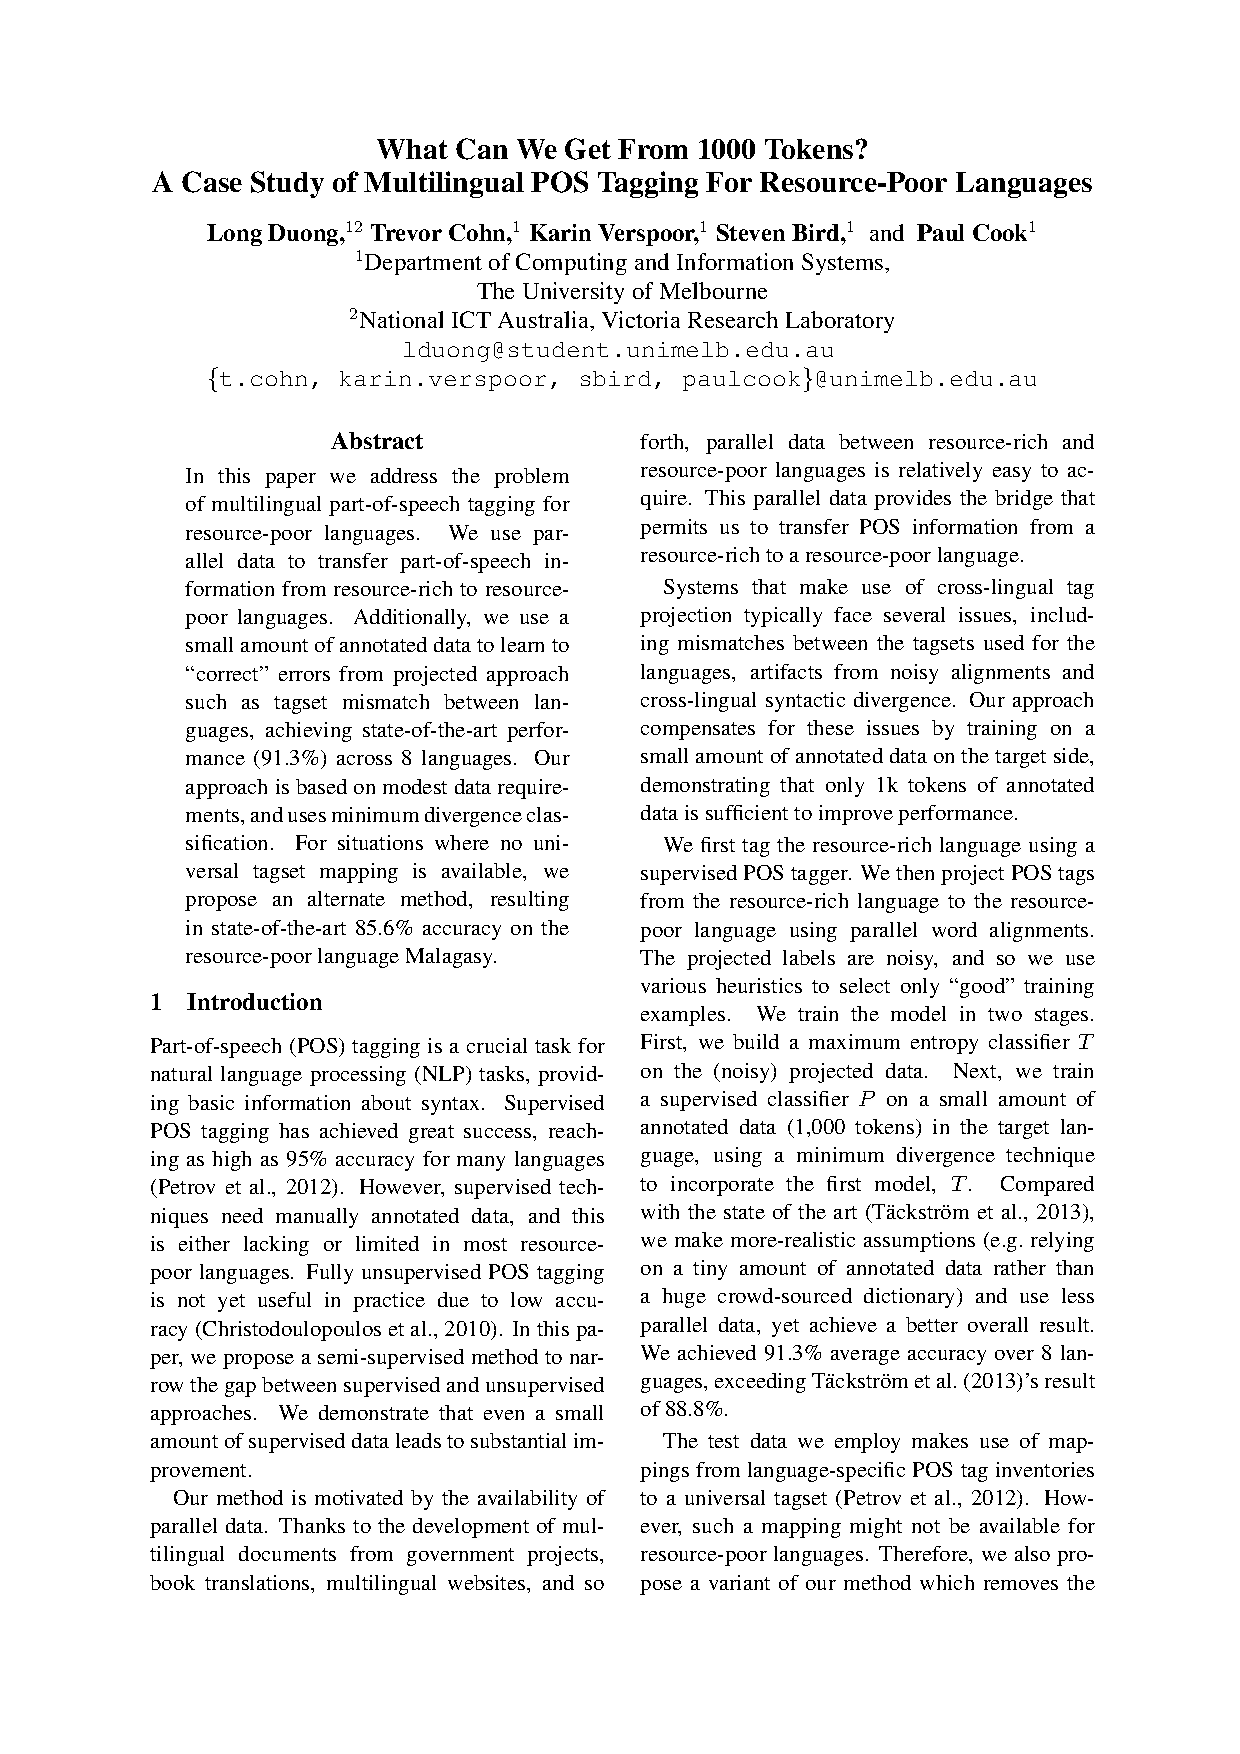
\includepdf[pages={1-},scale=1,pagecommand={\thispagestyle{plain}}]{Papers/emnlp14.pdf}
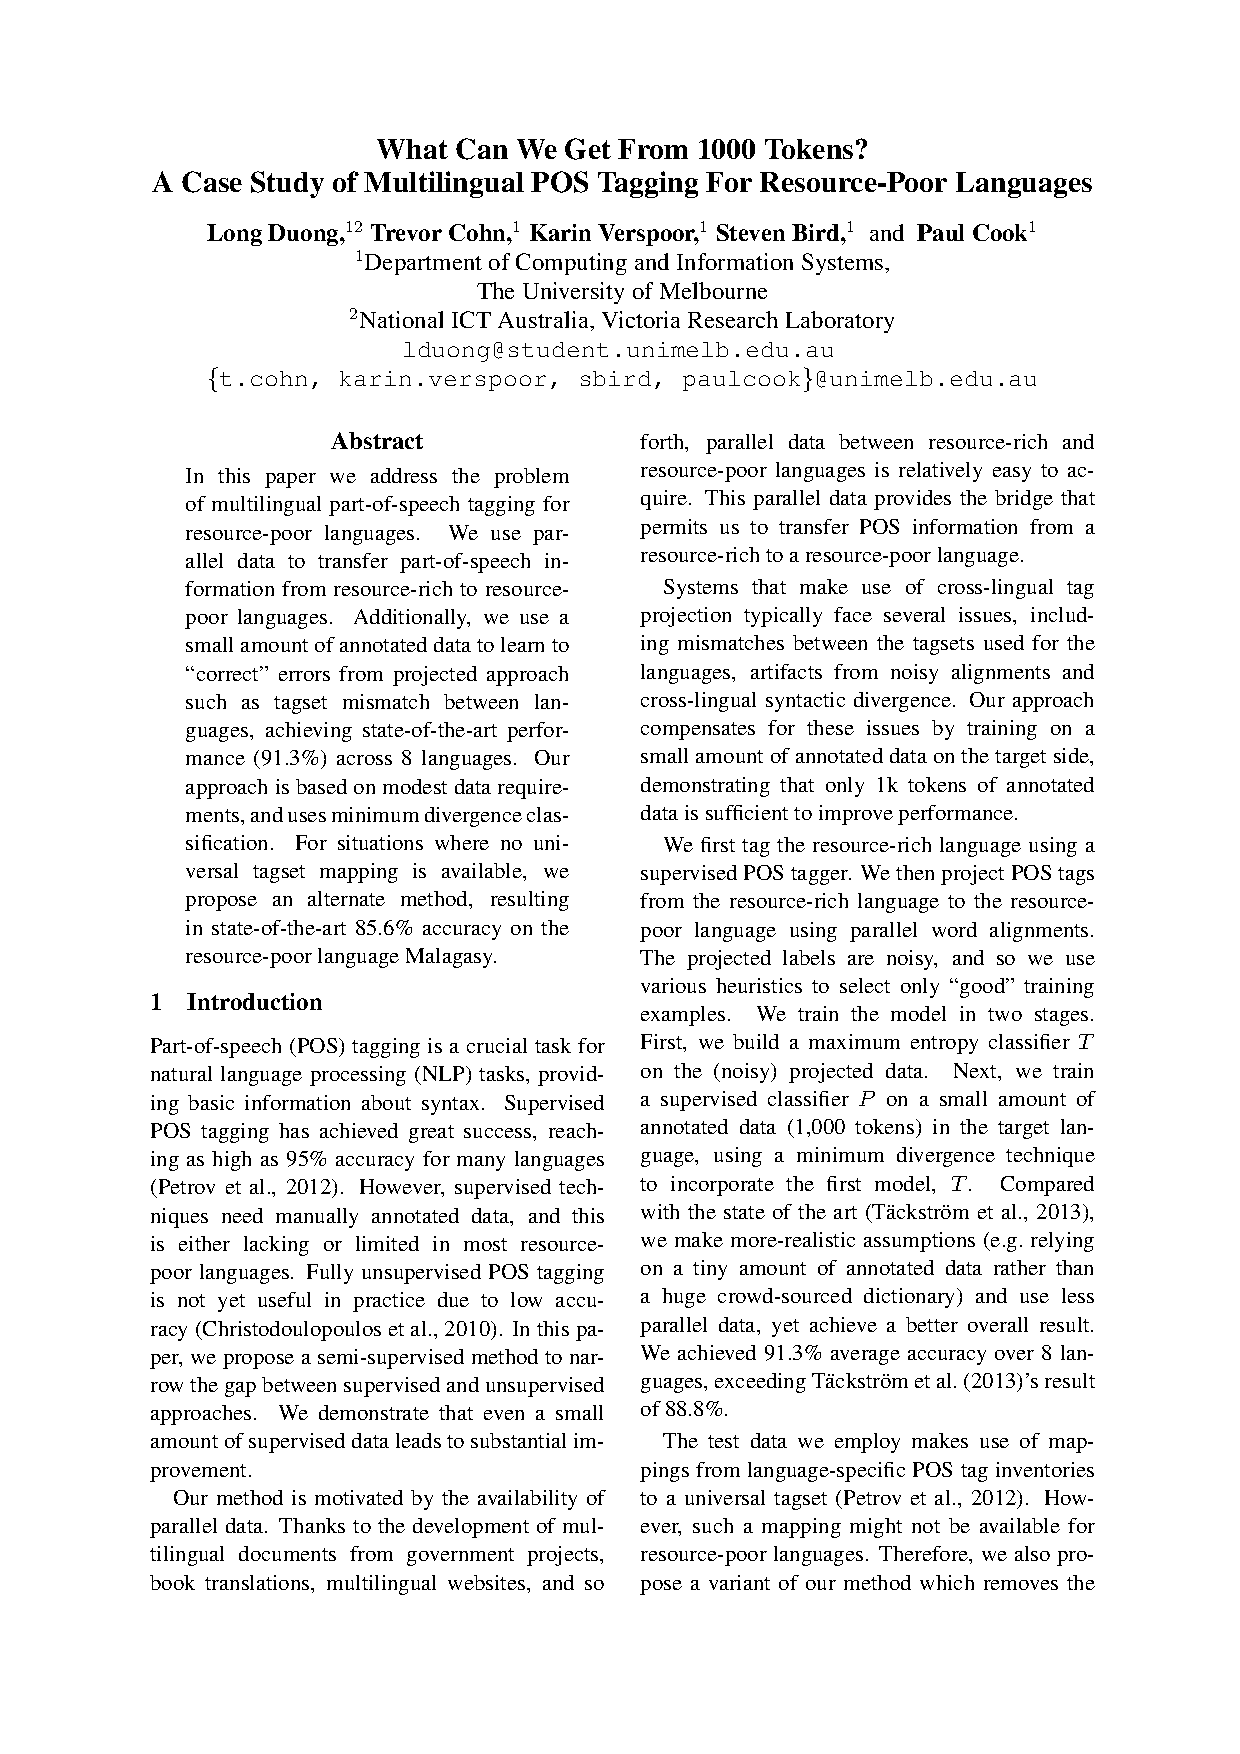
\includepdf[pages={1-},offset=0mm -7mm,scale=0.95,pagecommand={}]{Papers/emnlp14.pdf}

%------------------------------------------------------------%
%------------------------------------------------------------%
%------------------------------------------------------------%


\section{ACL 2015 -- Low Resource Dependency Parsing}
\label{sec:acl15}

\begin{quote}
Long Duong, Trevor Cohn, Steven Bird, Paul Cook. 2015. Low Resource Dependency Parsing: Cross-lingual Parameters Sharing in a Neural Network Parser. In\textit{ Proceeding of the 53rd Annual Meeting of the Association for Computational Linguistics (Volume 2: Short Papers)}.  845--850, Beijing, China
\end{quote}
\subsubsection{Research process}
% Joint training ...
After part-of-speech (POS) tagging, dependency parsing is the natural extension informing deeper layer of syntax. Working on dependency parsing is significantly 
harder compared with POS tagging. Instead of just outputting the tag label, we have to predict the tree-like structure of the sentence. Since we have successfully 
applied transfer learning for POS tagging taking advantage of small annotated corpus, the natural question is, can we do the same thing for dependency 
parsing. This paper forms a part of solving the second task about dependency parsing. 

In this paper, I design and run experiments. Other co-authors which are my supervisors contribute ideas during our weekly 
meeting and participated in the paper writing. 

\subsubsection{Retrospective view}
It is great observing that transfer learning technique through regularization terms is still applicable for dependency parsing task. Moreover, we only 
require the same POS annotation and dependency type between source and target language. This is a much better 
assumption compared with parallel data as used in ~\emnlpiv\ paper. Nevertheless, this paper still suffer similar drawback with the assumption of 
small annotated corpus in the target language. However, since annotating dependency treebank is much more costly and time consuming than POS annotation, 
applying our technique instead of annotating more data, is more compelling.  

% Independent of parallel data 
% Cost for dependency is higher ... 
% We haven't tested the joint training (cascade training) 

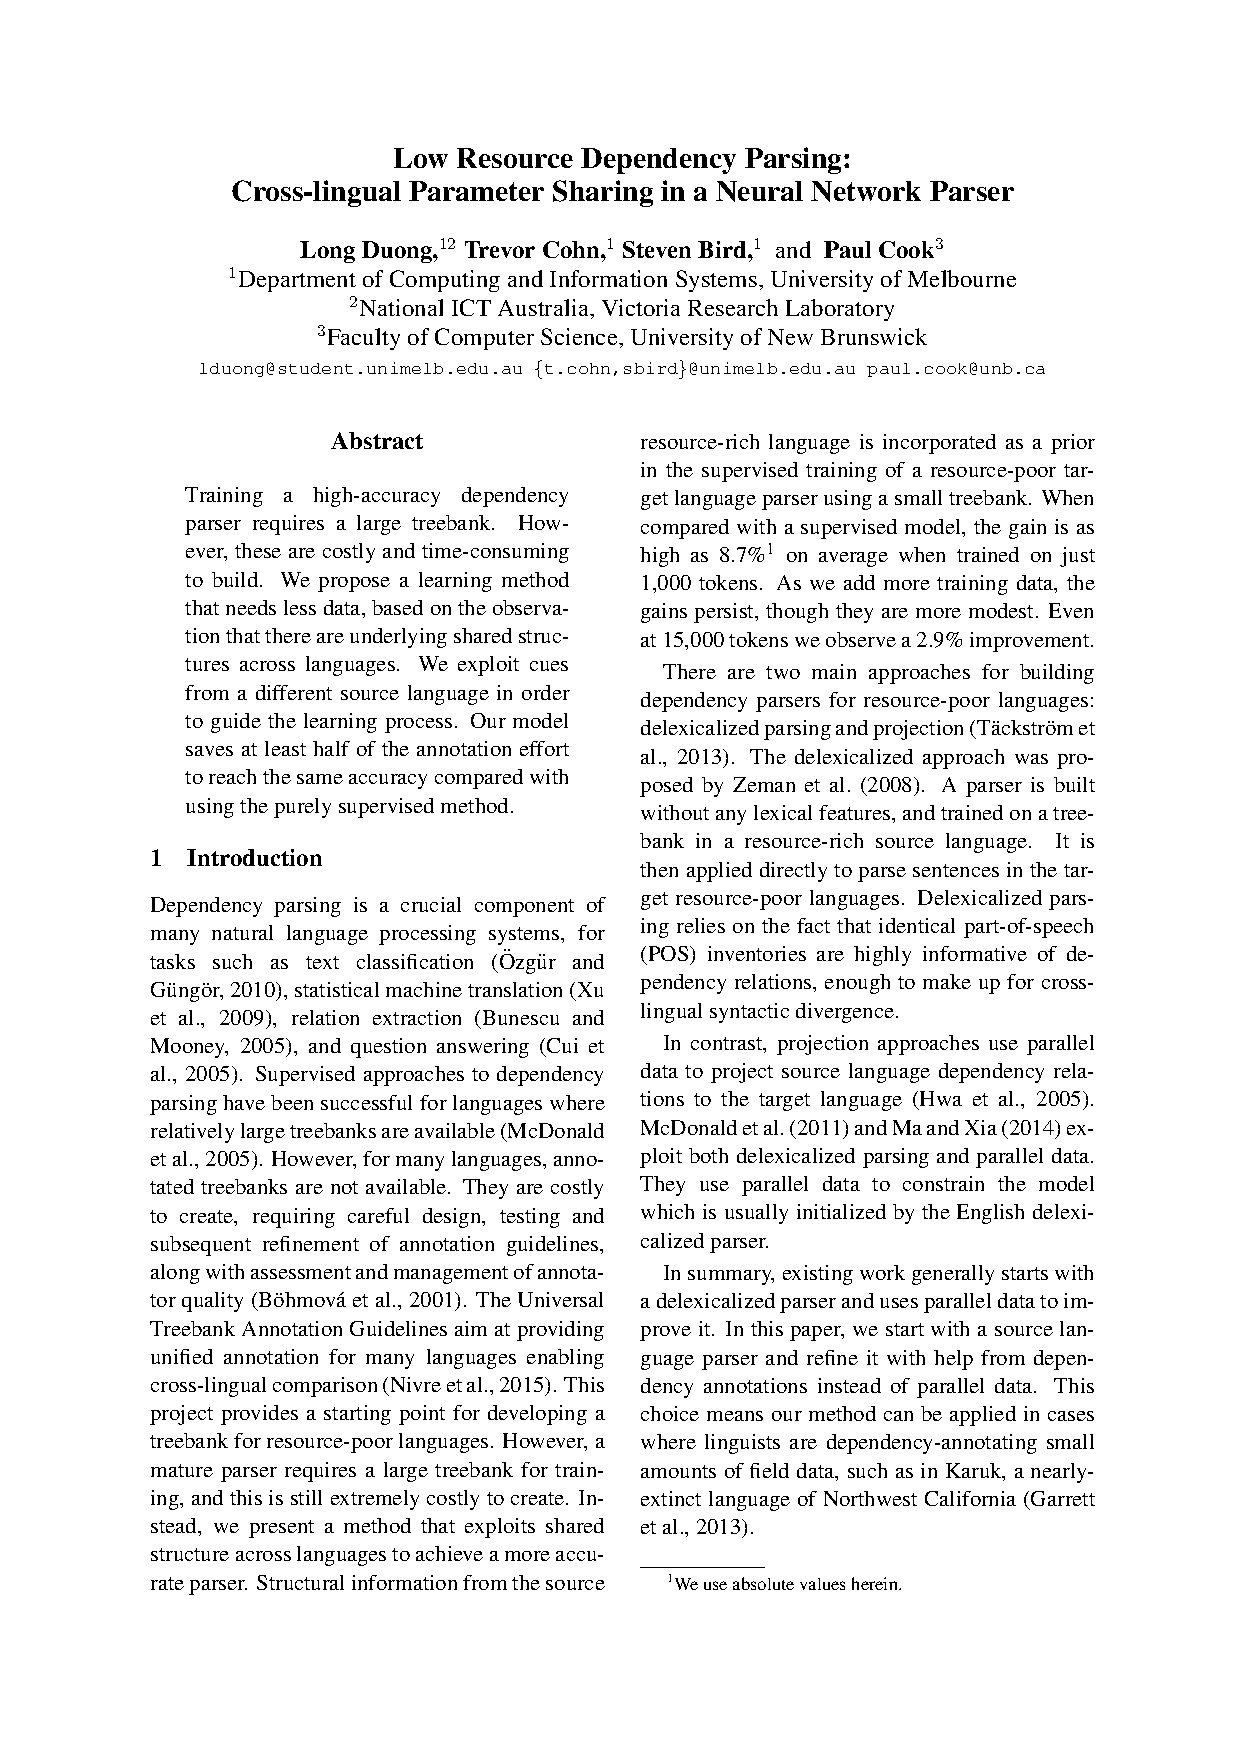
\includepdf[pages={1-},offset=0mm -7mm,scale=0.95,pagecommand={}]{Papers/acl15.pdf}

%------------------------------------------------------------%
%------------------------------------------------------------%
%------------------------------------------------------------%

\section{EMNLP 2015 -- Universal Dependency Parsing}
\label{sec:emnlp15}
\begin{quote}
Long Duong, Trevor Cohn, Steven Bird, Paul Cook. 2015. A Neural Network Model for Low-Resource Universal Dependency Parsing. In \textit{Proceedings of the 2015 Conference on Empirical Methods in Natural Language Processing}. 339--348, Lisbon, Portugal.
\end{quote}

\subsubsection{Research process}
In our \aclv\ paper, we train the model in the cascade style where source language parser is trained first and then used as the prior for the target language 
parser. However, we might benefit more from jointly train the source and target language together as this allows better 
parameter sharing, which is the motivation for this paper. 

In this paper, I design and run experiments. Other co-authors which are my supervisors contribute ideas during our weekly 
meeting and participate in the paper writing. 

\subsubsection{Retrospective view}
As shown in the paper, joint training is substantially better than cascade training across various data size. Also, joint training is more flexible, we can 
even relax the requirement of the same POS or dependency type annotation imposed in cascade training in \aclv\ paper. The model can automatically learn the 
annotation mapping between source and target language as part of the training. However, it is usually slower and more challenging to efficiently train the 
join model. Moreover, in this paper, we mainly compare with prior work using similar neural network transitional based parser. Despite the fact that the 
proposed joint model is generic and can apply to various architectures, how this work apply to or compare  with prior work using different parsing 
architecture such as graph based, is unknown. 
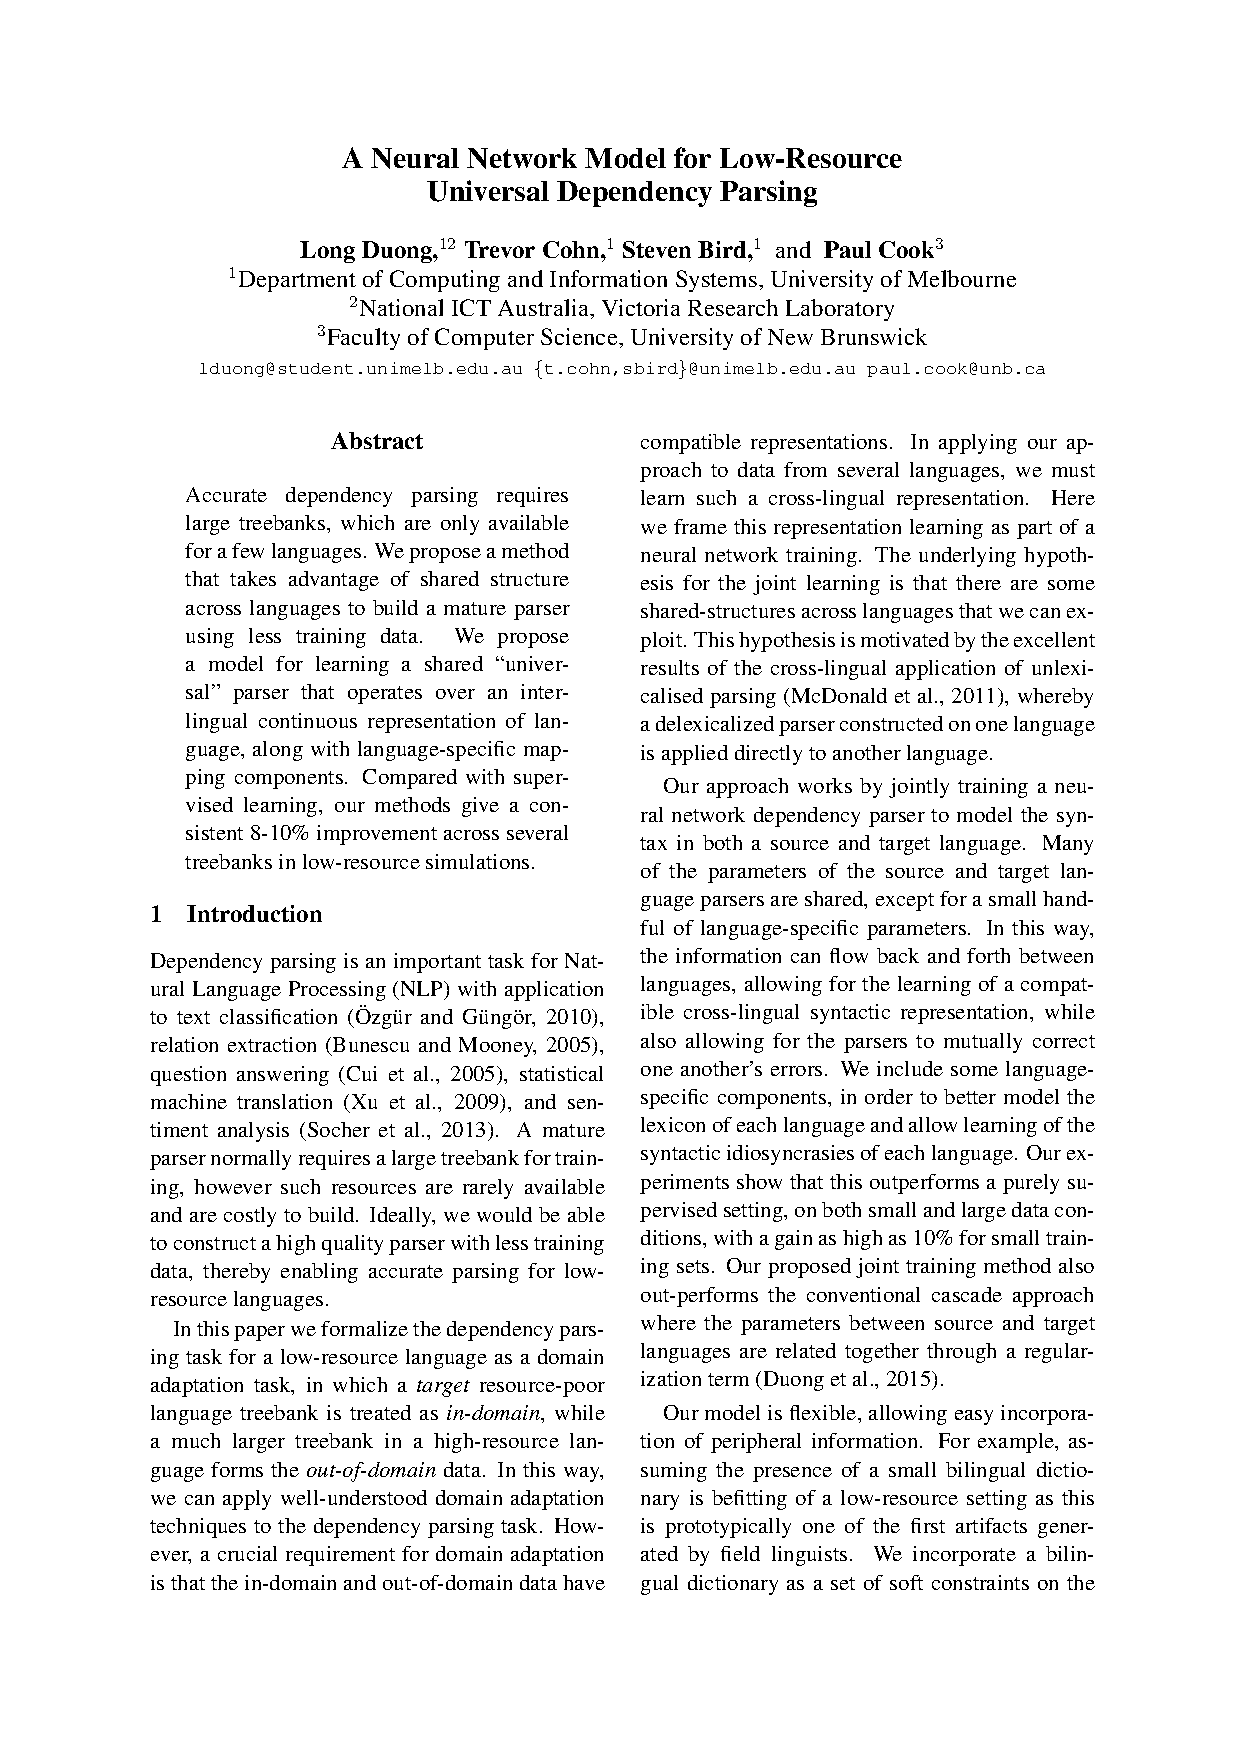
\includepdf[pages={1-},offset=0mm -7mm,scale=0.95,pagecommand={}]{Papers/emnlp15.pdf}

%------------------------------------------------------------%
%------------------------------------------------------------%
%------------------------------------------------------------%


\section{CoNLL 2015 --  Unsupervised Dependency Parsing}
\label{sec:conll15}
\begin{quote}
Long Duong, Trevor Cohn, Steven Bird, Paul Cook. 2015. Cross-lingual Transfer for Unsupervised Dependency Parsing Without Parallel Data. 
In \textit{Proceedings of the Nineteenth Conference on Computational Natural Language Learning (CoNLL 2015)}. 113--122, Beijing, China. 
\end{quote}

\subsubsection{Research process}
In both \aclv\ and \emnlpv\ papers, we assume a small annotated treebank in the target language. However, this treebank might not be available for 
many low-resource languages. That is why we want to further relax this assumption, motivating this paper for unsupervised dependency parser. 

In this paper, I design and run experiments. Other co-authors which are my supervisors contribute ideas during our weekly 
meeting and participate in the paper writing. 

\subsubsection{Retrospective view}
% Make much different in the downstream application ? 
It is surprising to see that delexicalized parser performs surprisingly well, achieves similar performance with supervised learning 
trained on 3000 tokens as in~\emnlpv\ paper. In this paper, we improve the delexicalized parser without using any additional resource. This 
is thank to the syntactic word embeddings that only requires the same POS annotation between source and target 
language. However, for a single source language the improvement is modest. The biggest 
gain is from taking advantage of multiple source languages. However, the gain is not consistent across languages and usually higher for languages that share 
some commonalities with source languages. 

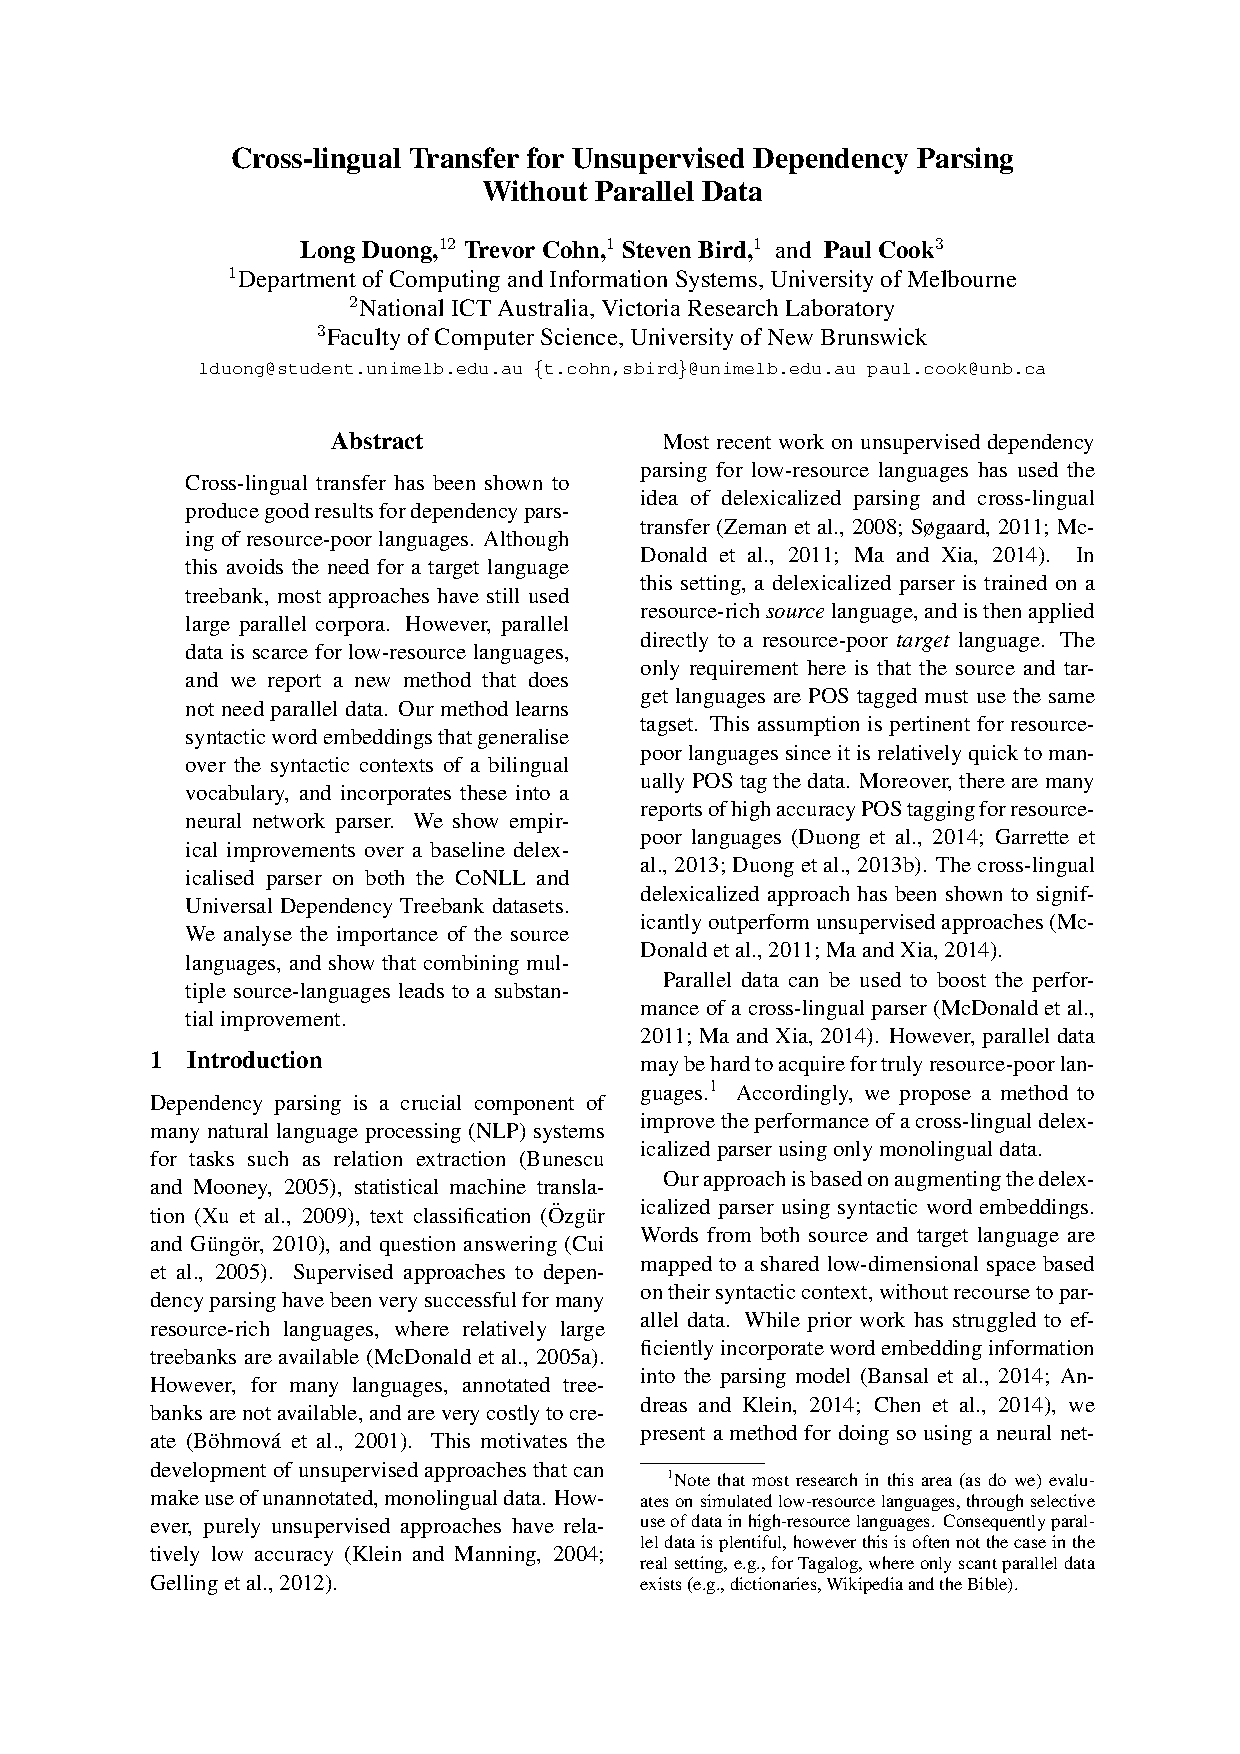
\includepdf[pages={1-},offset=0mm -7mm,scale=0.95,pagecommand={}]{Papers/conll15.pdf}


%------------------------------------------------------------%
%------------------------------------------------------------%
%------------------------------------------------------------%


\section{EMNLP 2016 -- Crosslingual Word Embeddings}
\label{sec:emnlp16}
\begin{quote}
Long Duong, Hiroshi Kanayama, Tengfei Ma, Steven Bird, Trevor Cohn. Learning Crosslingual Word Embeddings without Bilingual Corpora. In \textit{Proceedings of the 2016 Conference on Empirical Methods in Natural Language Processing (EMNLP 2016)}. 1285--1295, Austin, Texas, USA\
\end{quote}

\subsubsection{Research process}
Transfer learning is the core idea of all our previous paper. Lexical transfer is one of the most important part. Investigating a better way to 
do lexical transfer would benefit not only POS tagging or dependency parsing but also many other transfer learning task, motivating this paper. 

This paper is done during my internship at IBM research -- Tokyo where they interested in transfer learning for their data mining system. I took the 
intership offer mainly because their research interest align well with the overall target of the thesis, aiming at solving the third task (crosslingual 
word embeddings). Aside from Steven and Trevor from Melbourne university, I also have Hiroshi and Tengfei as my IBM side supervisor. In this paper, I implement the algorithm and run all experiments. Other co-authors contribute ideas during our weekly meeting and participate in the paper writing. 

\subsubsection{Retrospective view}
This paper uses dictionary for building crosslingual word embeddings applied successfully for both intrinsic tasks (monolingual similarity and bilingual lexicon
induction task) and extrinsic task (crosslingual word embeddings). However, because of space constrain, we haven't evaluated on syntactic extrinsic task such as 
crosslingual dependency parsing. Moreover, crosslingual word embeddings currently only work for a pair of language, it is shown in~\conllv\ that crosslingual word embeddings for multiple languages are more beneficial in transfer learning. 
%In addition, the experiment with low-resource language Serbian need to compare with several other dictionary based cross-lingual word embeddings such as 
% Low-resource scenario 
% dictionary is more widely available than parallel data 
% should test it on dependency parsing task  => OK 
% Test Bilingual Lexicon Induction task (some overlaping with test set)

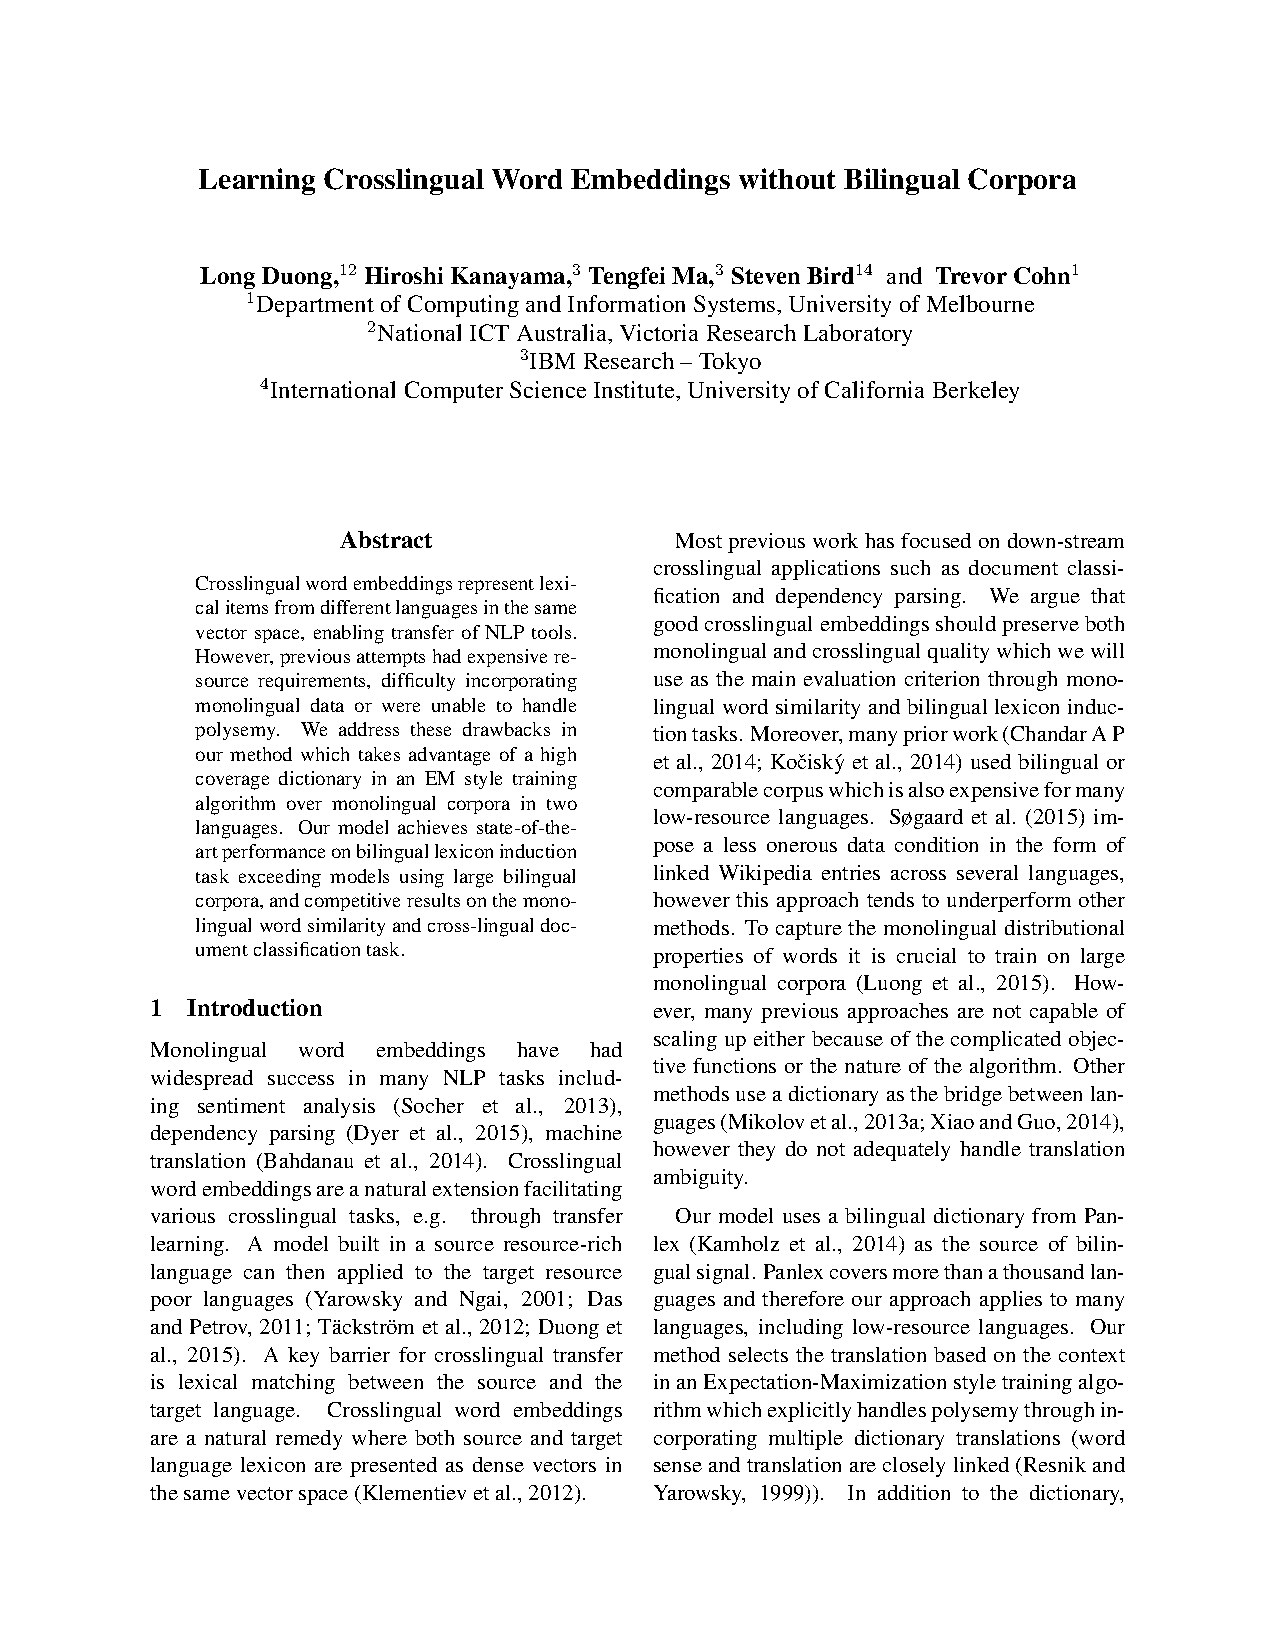
\includepdf[pages={1-},offset=0mm 0mm,scale=1,pagecommand={}]{Papers/emnlp16.pdf}

%------------------------------------------------------------%
%------------------------------------------------------------%
%------------------------------------------------------------%

\section{EACL 2017 -- Multilingual Word Embeddings}
\label{sec:eacl17}
\begin{quote}
Long Duong, Hiroshi Kanayama, Tengfei Ma, Steven Bird, Trevor Cohn. Multilingual Training of Crosslingual Word Embeddings (to appear). In \textit{Proceedings of the 2017 Conference on European Chapter of the Association for Computational Linguistics (EACL 2017)}. Valencia, Spain. 
\end{quote}

\subsubsection{Research process}
This work is the extension of our \emnlpvi\ paper, also conducted during my time at IBM research Tokyo. Basically, we want to extend crosslingual word embeddings to more than two languages. Besides, we want to better position ours with prior work using more evaluation metric focusing on downstream applications. 

In this paper, I implement the algorithm and run all experiments. Other co-authors contribute ideas during our meetings and participate in the paper writing. 

\subsubsection{Retrospective view}
We have successfully extend the model for multilingual training of crosslingual word embeddings. However, this paper didn't compare the training complexity. 
The training complexity of both post-hoc unification methods (e.g. linear transformation or CCA) and multilingual join training grow linearly with the 
number of language. However, post-hoc training is much easier to parallellize since each language can be trained separately. Scaling up multilingual join 
training to massive number of languages (e.g. 100 languages) is definitely more challenging. In addition, while post-hoc unification methods performance 
is almost constant regardless of number of languages, how the performance changes with multilingual join training when add more languages, is unknown. 

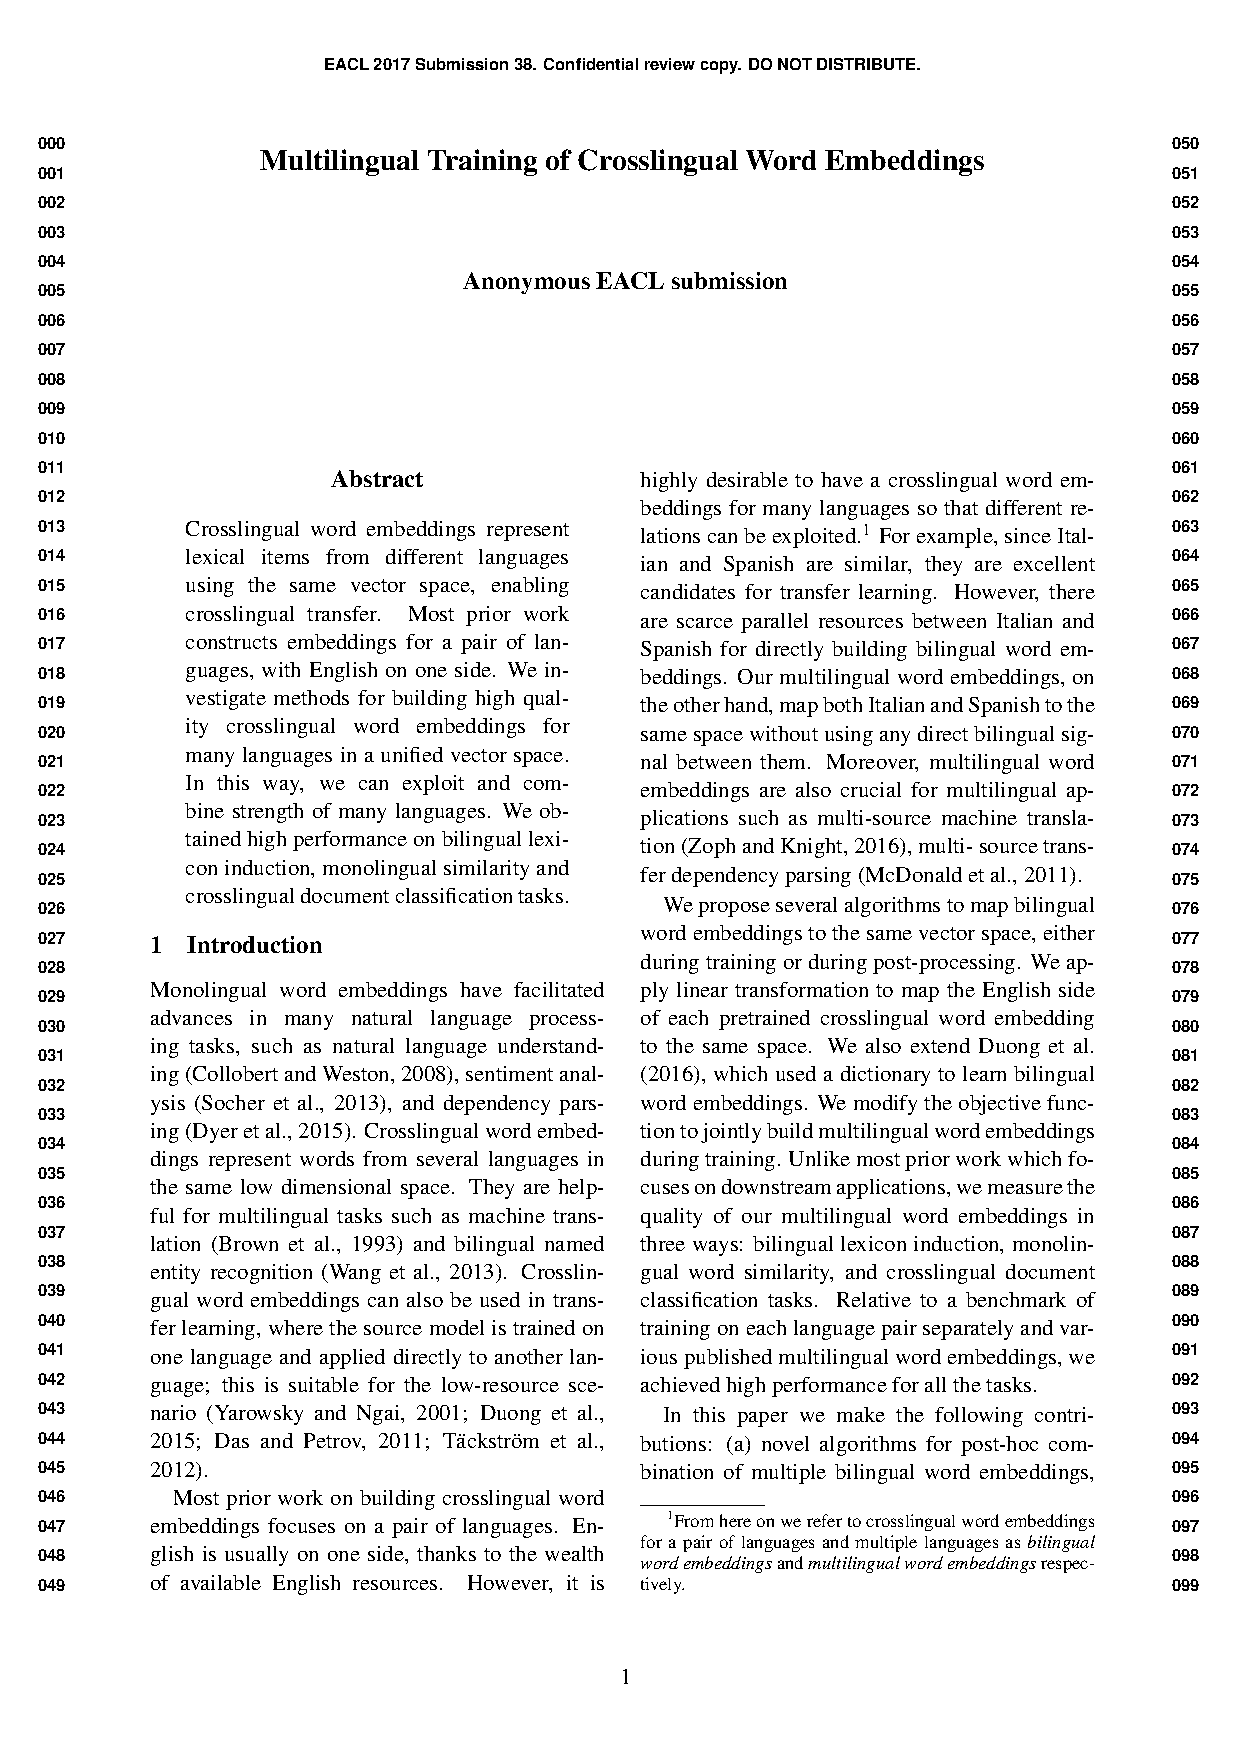
\includepdf[pages={1-},offset=0mm -7mm,scale=0.95,pagecommand={}]{Papers/eacl17.pdf}

%------------------------------------------------------------%
%------------------------------------------------------------%
%------------------------------------------------------------%

\section{NAACL 2016 -- Speech Translation}
\label{sec:naacl16}
\begin{quote}
Long Duong, Antonios Anastasopoulos, David Chiang, Steven Bird and Trevor Cohn. An Attentional Model for Speech Translation Without Transcription. In\textit{ Proceedings of the 2016 Conference of the North American Chapter of the Association for Computational Linguistics: Human Language Technologies (NAACL-HLT 2016)}. 949--959, San Diego, USA.
\end{quote}

\subsubsection{Research process}
This paper aim at solving the forth task in our thesis, processing unwritten languages. This is a very challenging task as we have to work directly on speech 
signal. We formalize the problem as sequence to sequence learning building upon~\namecite{DBLP:journals/corr/BahdanauCB14}. 

This paper is the outcome of the project started during my internship at ICSI, UC Berkeley. Aside from Steven and Trevor, this is also the join work with Antonios and David from Notre Dame University. Antonios helps with preparing the dataset, evaluation scripts and calculate baselines. I implement the algorithms and run experiments adapting Trevor's work on neural machine translation~\cite{cohn-EtAl:2016:N16-1} for speech. Other co-authors contribute ideas during our meetings and participate in the paper writing. 

\subsubsection{Retrospective view}
Despite the fact that we achieve good result on phoneme level representation, the result on experiment applied directly on speech signal is unsatisfying for both 
translation quality and alignment quality. While the idea is novel and interesting, it seems that we bit off more than we could chew given the small size of speech 
data and the data hungry nature of deep neural approach. I have co-authored another paper with Antonios and David, taking simpler approach using Expectation-Maximization which achieve better result~\cite{anastasopoulos-chiang-duong:2016:EMNLP2016}. However, I contributed less than 50\%, as such shouldn't be counted toward my PhD.

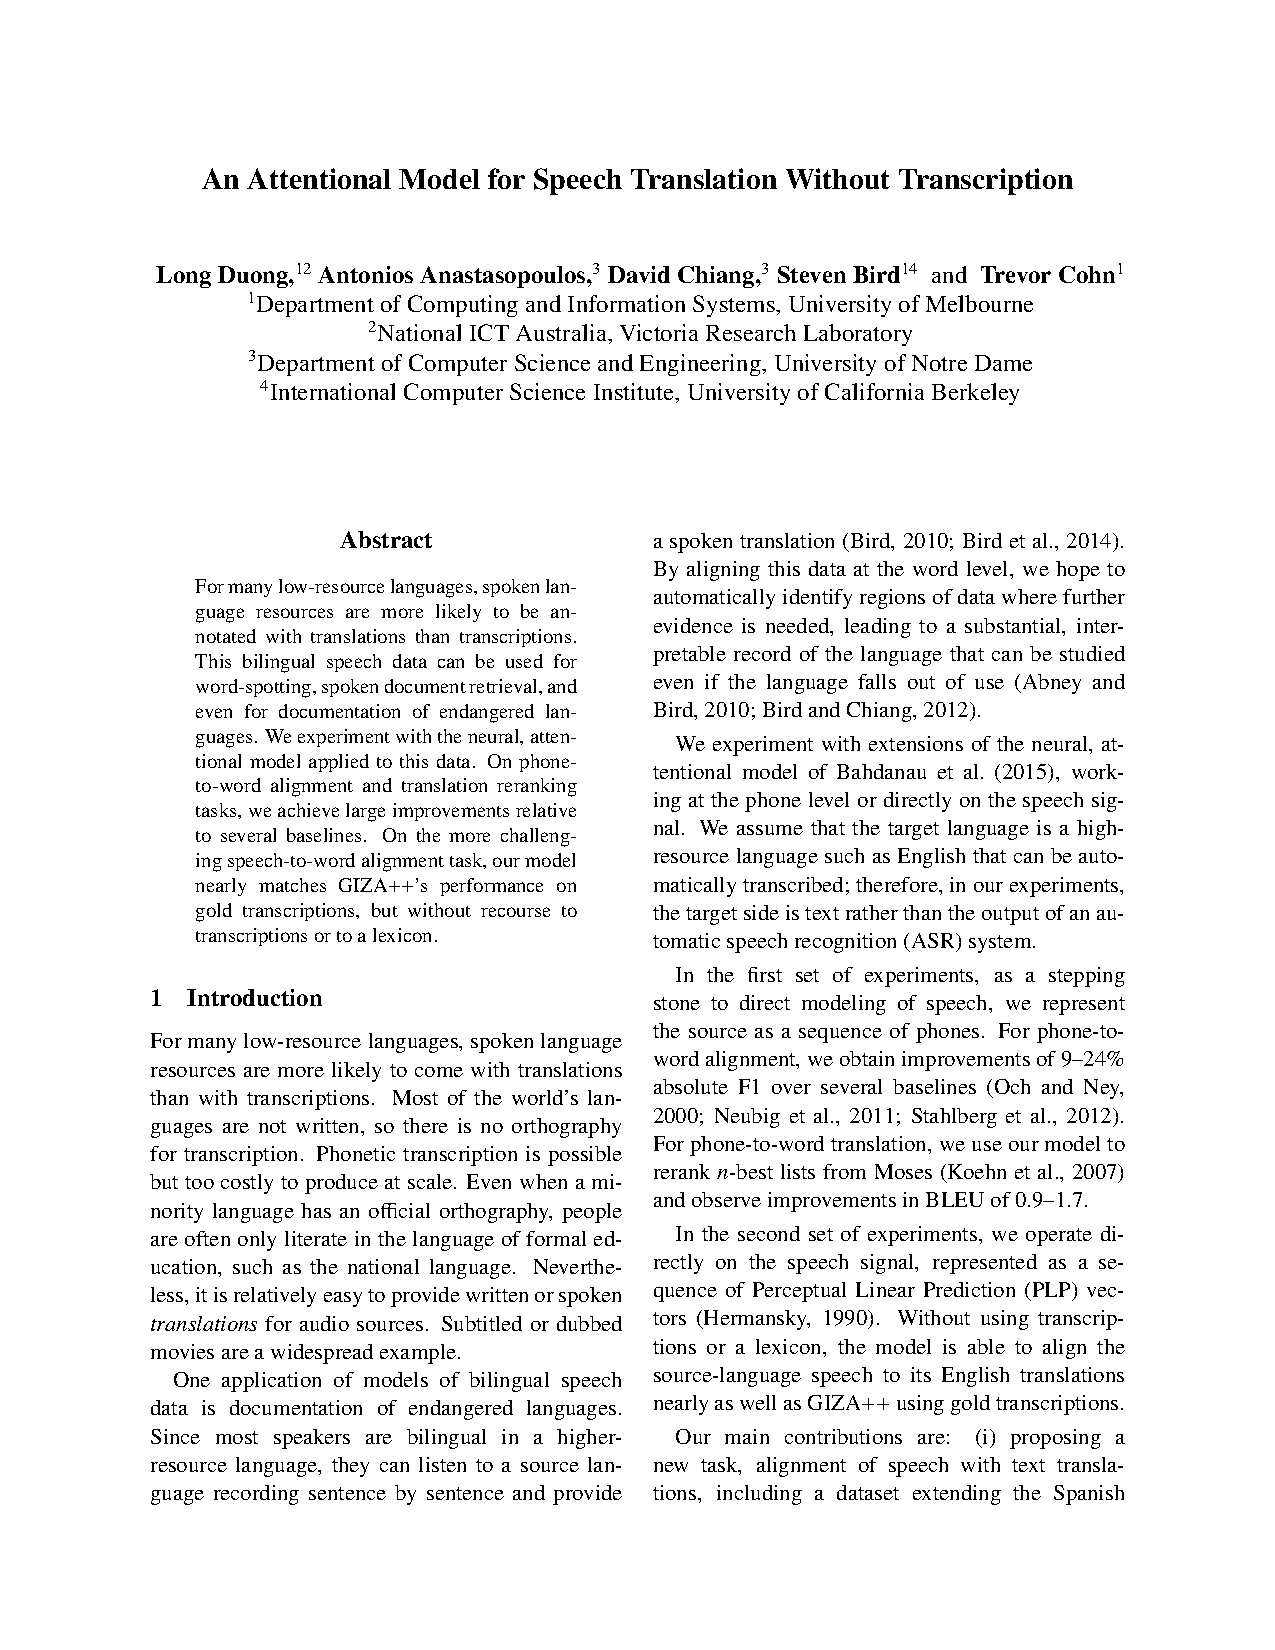
\includepdf[pages={1-},offset=0mm 0mm,scale=1,pagecommand={}]{Papers/naacl16.pdf}

%%%%%%%%%%%%%%%%%%%%%%%%%%%%%%%%%%%%%%%%%%%%%%%%%%%%%
%%%%%%%%%%%%%%%% NEW CHAPTER %%%%%%%%%%%%%%%%%%%%%%%%
%%%%%%%%%%%%%%%%%%%%%%%%%%%%%%%%%%%%%%%%%%%%%%%%%%%%%

\chapter{Discussions and Conclusions}
\label{chap:conclusion}
In this chapter, we conclude our thesis by linking it back to the introduction, answering the questions such as (a) How did the list of publications in \S\ref{chap:research_summary} fit into the thesis's aim? (b) How did the research questions proposed in the introduction (\S\ref{chap:introduction}) get 
answered? and (c) How well did we cover four tasks (POS tagging, dependency parsing, crosslingual word embeddings and unwritten language processing) proposed earlier? Moreover, we also critically evaluate the contributions and enumerate some possible directions
for future work. 

\section{Evaluation of Contribution}
\label{sec:evaluation_contribution} 
In this thesis, we have looked at different facets of processing low-resource languages. Our contribution are four folds. 
\begin{itemize}
\item The algorithm to effectively incorporate complementary resource such as parallel corpora or language relatedness, to the low-resource languages. We exploit transfer learning framework taking advantage of large annotated corpus in the source language and some annotations in the target language. We have shown that these methods can even apply to improve 
the performance on high resource languages. 
\item The algorithm to improve the unsupervised learning for low-resource languages taking advantages of crosslingual syntactic embeddings and crosslingual 
word embeddings applied successfully for dependency parsing and document classification. 
\item The algorithm to solve many low-resource specific problems such as annotation mismatch between source and target language or extremely low-resource scenario of unwritten languages.
\item Several new datasets such as English-Serbian bilingual lexicon induction dataset, speech to text alignment corpus. 
\end{itemize}

\subsection{Task coverage}
% COVER ALL 4 TASKS, what is task coverage ....
\paragraph{POS tagging} We cover all four tasks proposed earlier. For the first task of low-resourced POS tagging, in our \emnlpiv\ paper, we propose a novel semi-supervised method building 
upon our prior work on unsupervised POS tagging~\cite{duongIJCNLP,Duongacl13}. Comparing with 
the state-of-the-art, who also take advantage of parallel data, we use more realistic assumption, less parallel data but achieve better result. 
In that paper, we also propose a novel tagset mapping algorithm, applied when source and target language use different tagset inventory. At the 
time of writing the paper, we achieved the state-of-the-art performance on the low-resource language Malagasy. 

\paragraph{Dependency parsing} For the second task of dependency parsing, in our \aclv\ paper, we proposed a semi-supervised methods exploiting parameters sharing in the 
neural network parser between source resource rich langauge and target resource poor language. The model was trained in the cascade style 
where source language model is trained first and used as the prior for the target low-resource language model. We shown that we can achieve 
more accurate parser using the same training data. In our \emnlpv\ paper, we further improved the performance in the semi-supervised setting. We modify 
the training such that source and target language parsers are jointly optimized, allowing better parameter sharing. We observed a consistent gain
of as high as 10\% across various data size in the low-resource setting. In that paper, we also shown that the word embeddings learned as part 
of the join training, capture meaningful syntactic phenomena, achieving high performance on verb similarity task. In the extreme case, where 
we do not have any annotated treebank, we proposed an unsupervised algorithm in our \conllv\ paper taking advantaging of the novel syntactic word 
embeddings without recourse to parallel data. When applied to the target low-resource language, we observed consistent improvement. In addition, 
if there are multiple source languages, we propose a method to combine them together which leads to substantial improvement. 

\paragraph{Crosslingual word embeddings}The third task which is learning crosslingual word embeddings, is covered by \emnlpvi\ and \eaclvii\ papers. While previous approaches have expensive resource requirements, 
high complexity objective function or unable to handle polysemy. We address all those drawbacks in our \emnlpvi\ paper, taking advantage of high 
coverage but noisy dictionary, in an Expectation-Maximization style disambiguation training over monolingual data in two languages. We shown that the 
learned embeddings are high quality, preserving both monolingual and bilingual distance. We achieved competitive results on unsupervised crosslingual 
document classification task without recourse to parallel corpora. Moreover, our proposed technique to combine embeddings during training can even be used for 
improving monolingual word embeddings. However, in \emnlpvi\ paper, we only consider building crosslingual word embeddings for a pair of language. 
It is more beneficial when we build crosslingual word embeddings for multiple languages which is addressed in our \eaclvii\ paper. We propose
several methods for building multilingual word embeddings including post-hoc combination and join-training. Using our multilingual word embeddings, we observed improvement in both unsupervised crosslingual document classification and unsupervised dependency parsing task. 

\paragraph{Unwritten language processing}The last proposed task of processing unwritten language is preliminary in our \naaclvi\ paper. After carefully evaluating the data requirement, we decide 
to model directly between speech signal from low-resource language and the target higher resource language translation. We experimented with the neural attentional model 
for this data. On the initial experiment where we assume phoneme transcription in the source language, we achieved large improvement relative to several 
baselines. On the more challenging speech-to-word modelling task, we shown that the model still capable of learning meaningful relations showing the feasibility 
of the this proposed tasks. 

\subsection{Research question revisited}
\textbf{Question 1}: How can we achieve more accurate model for low-resource languages using less annotated data? 
\begin{itemize}
\item In \emnlpiv\ paper, we shows that bilingual corpora when available can be used to transfer the annotation from source resource rich language to target 
resource poor language. We observed improvement using this parallel corpora together with a small part-of-speech annotated corpus in the target language. Even if 
the annotation is different between source and target language, we can also automatically learn the mapping as part of the training. 
\item 	In \aclv\ and \emnlpv\ papers, we introduce the concept of ``universal parser`` where as there are a share underlying linguistic structure across languages. 
Using this share structure together with a small annotated data in the target language, we obtained a more accurate model.  
\end{itemize}

\textbf{Question 2}: How can we achieve more accurate model for low-resource languages without annotated data?

\begin{itemize}
\item In \conllv\ paper, we show that even in the extreme case where there are not any annotated data, we can still improve the performance of unsupervised dependency parser by relexicalizing the 
delexicalized model using crosslingual syntactic word embeddings. In addition, we can even further improvement the performance when multiple source languages are available exploiting transfer learning using multiple source languages. 
\item Transfer learning has been a successful technique applying to improve performance on low-resource languages, in \emnlpvi\ paper, we investigate a new way to build crosslingual word embeddings used for lexical transfer. Crosslingual word embeddings can be used in transfer learning applied for many unsupervised natural 
language processing task. In \emnlpvi\ paper, we demonstrate the usability in unsupervised crosslingual document classification. 

\item In \eaclvii\ paper, we extended the crosslingual word embeddings training to multiple languages. We show that multiple source languages can be used to further improve the performance for unsupervised learning demonstrated successfully for crosslingual document classification and crosslingual dependency parsing tasks.  
\end{itemize}

\textbf{Question 3}: What can we learn from unwritten languages?
\begin{itemize}
\item In our \naaclvi\ paper, we proposed the new task of learning directly from unwritten language speech and the translation in the higher resource language. Despite preliminary, we shown that meaningful alignments can be learned directly, providing the proof of feasibility. This work provide the stepping stone for 
subsequent work in the field. % such as~\namecite{anastasopoulos-chiang-duong:2016:EMNLP2016}. 
\end{itemize}

\section{Future Work}
\label{sec:futurework}
This section enumerates some possible directions for future work. 
\subsection{More evaluations for low-resource languages} 
One of the weakness of this thesis is that much work is evaluated on the simulated low-resource scenario.
This is the common strategy for low-resource natural language processing since it is hard to get the gold evaluation data 
for a real low-resource language. We are lucky to have Malagasy part-of-speech evaluation corpus for our \emnlpiv\ paper. 
For the dependency parsing task, we mainly evaluated on European languages, while Hungarian and Irish can be considered as  
low-resource languages, other languages such as Czech or French are not. 
The new version of universal dependency 
treebank v1.3~\cite{11234/1-1699} has some candidate low-resource languages such as Buryat, Coptic, Kazakh or Sanskrit
which have very modest treebank size (less than 1000 annotated sentences). We would like to evaluate our existing approach 
proposed in ~\aclv, \emnlpv\ and \conllv\ papers to those languages in both semi-supervised and unsupervised setting. 

In our \emnlpvi\ paper, we included Serbian as an example of low-resource language. The performance on bilingual lexicon induction 
task on English-Serbian is still acceptable given the small size of dictionary and monolingual data. However, we want to evaluate  
on downstream applications for Serbian such as dependency parsing or document classification. However, this would requires manual 
test data annotation. Our \eaclvii\ paper proposes methods for multilingual training for crosslingual word embeddings, extending 
~\emnlpvi\ paper. However, in that paper, we only experimented with high resource European languages. For the future work, we would 
like to extend to more low-resource languages outside of European languages. 

In our \naaclvi\ paper, we experimented with Spanish speech and English translation. This is convenient as we can get Spanish phoneme 
for the upper bound experiments. However, it would be interesting to apply for real low-resource languages.~\namecite{Blachon201661} used 
an extended version of Aikuma~\cite{bird-EtAl:2014:W14-22} to collect more than 80 hours of speech and the translation from Congo-Brazzaville
language. As the future work, we want to apply our approach to this dataset. 


\subsection{Real-world evaluation}
Similar with many work in the literature when working with low-resource languages, we make assumptions. 
For the future work, we would like to systematically test and verify these assumptions in the real low-resource language scenario.
In our~\emnlpiv\, \aclv\, \emnlpv\ paper, given a small treebank in the target language, we employ various approaches, incorporating 
complementary information to arrive with more accurate model. However, we have not taken the cost of applying our proposed approaches to 
the model. %In fact, what we need to do is calculate the effort in term of man power or money to employing our techniques, 
%assuming it is $X\$$. We need to compare the performance between (a) use this $X\$$ to annotate more data and apply any simple supervised 
%learning and (b) using this $X\$$ to employ our proposed approaches. Only in this way, it would be a fair comparison. However, correctly 
What we would like to try is that given a task such as POS tagging or dependency parsing, and the expected accuracy e.g. 90\%, calculate the amount 
of time or money needed to finish the task with and without our proposed methods. In another way, we want to quantify our work, not in term 
of accuracy but in term of time or money which is usually used in real-world applications. 

\subsection{Filling in  the gap}
% Crosslingual word embeddings with our parsing model ...
In our \conllv\ paper, we use crosslingual syntactic embeddings to improve performance of unsupervised dependency parsing. In our \emnlpvi\ and \eaclvii\ paper, 
we propose the crosslingual word embeddings using bilingual dictionary. The simple extension is just use our proposed crosslingual word embeddings instead of 
crosslingual syntactic embeddings. 

In our \emnlpv\ paper, we jointly train the dependency parser for a pair of languages. The output parser can be understood as combination of two parts. The universal
parser part that parse universal language and the conversion part that convert a language to the universal language. It would be interesting to jointly train the model with many source languages. In this way, we expect to truly learn the universal parser. 

In our \emnlpvi\ and \eaclvii\ paper, we build the crosslingual word embeddings using dictionary from Panlex. However, we can even further improve 
the dictionary coverage by combining Panlex with bilingual dictionary from Wiktionary and bilingual dictionary induced from parallel data. Since our model 
has the capability to disambiguate noisy dictionary translations, this will likely boost the performance. 

In our \naaclvi\ paper, there are several problems with the current model we would like to investigate. First we want to change to global objective function 
instead of current local objective function. Basically, the current objective function is the language model which additionallly condition on the speech signal. 
This local objective function can not ensure the global quality of the generated translations. Second, the current training and testing procedures are not consistent. During training, the model condition on the previous ground truth word to generate the next word. During testing, the model instead condition on the generated words which is prone to errors. These problems also observed in~\namecite{wiseman-rush:2016:EMNLP2016} and~\namecite{DBLP:journals/corr/BahdanauBXGLPCB16}. Last, we want to investigate more on decoder such that it can memorize longer history, ensuring higher quality translations. 

\section{Conclusion}
In this thesis, we have proposed several methods to automatically process low-resource languages. We have not covered all the natural language 
processing tasks, but the proposed methods using transfer learning are universal and applicable for many tasks. We also look at low-resource
languages on different level of resource requirements including semi-supervised learning, unsupervised learning and our preliminary attempt at unwritten languages. 
% Strength and Weakness of the thesis 
While most claims in this thesis is backed up by the set of publications on top-tier conferences, this thesis still lack of analysis on real low-resource 
languages which is also addressed as the future work. We believe that when evaluating on real low-resource languages, many unexpected challenges will arise and need to take into consideration. 
% What is the taking home lesson
The taking back home lesson is that (a) processing low-resource language is very hard but transfer learning is one possible solution. (b) There are many complementary resources we can use to compensate for the lack of annotated data. (c) Processing low-resource languages usually overlooked by the set of assumptions such as availability of writing system.  
% Impact on the field ? 
We hope our thesis will help to drive the field forward, becoming the stepping stone for future research on low-resource natural language processing. There are some
notable researchs that already benefited from our initial research on POS tagging~\cite{DBLP:conf/conll/FangC16,Pecheux2016,zhang-EtAl:2016:N16-13,bacskaya2016semi}, Parsing~\cite{DBLP:journals/corr/GillickBVS15,Guo:2016:RLF:3016100.3016284,TACL892,DBLP:journals/corr/GuoCWL16,ledbetter-dickinson:2016:BEA11,TACL917}, unwritten language processing~\cite{DBLP:journals/corr/BansalKGL16,adams-EtAl:2016:EMNLP2016,anastasopoulos-chiang-duong:2016:EMNLP2016,Wilkinson+2016}. 

% Personal gain 
%Personally, I learned alot from this PhD including graphical model, Bayesian inference, domain adaptation, structure prediction and deep neural network. I also expand my knowledge about more NLP tasks such as machine translation, POS tagging, dependency parsing, document classification, representation learning, word sense disambiguation, speech recognition, natural language understanding, language and vision. During my PhD, I also expand international collaborations through my two internships (at IBM Research -- Tokyo and ICSI, UC Berkeley), set of international conferences I attended (EMNLP 14, EMNLP 15, ACL 15, ConLL 15, EMNLP 16) and set of talks I gave (at Google, Ebay, IBM, Monash University, UC Berkeley and NII -- Tokyo). I also develop academic experience through teaching at CIS department, University of Melbourne and serving as program committee on several conferences such as EMNLP 15, ACL 16, NAACL 16, COLING 16 and ALTA 16. Looking back, I can say that I enjoyed my PhD. 

% 




% Chapter 2: Background and litereature review 
%%% intro.tex
\chapter{Background and Literature Review}
%%%%%%%%%%%%%%%%%%%%%%%%%%%%%%%%%%%%%%%%%%%%%%%%
\label{chap:backGround}
This chapter reviews methods for monolingual and multilingual POS tagging. It provides background knowledge that is necessary for the next chapters. Monolingual POS tagging aims at building a tagger for a single language, and it does not take into account the relationship with other languages. Monolingual POS tagging is language-specific, which might used languages rules/heuristics to improve performance. Multilingual POS tagging, on the other hand, favoring a language-independent approach. It takes into account the relation between languages and aims at building taggers for many languages. More specifically, multilingual taggers build a tagger for one language based on data from other languages. Monolingual POS taggers exploit supervised, semi-supervised or unsupervised methods depending on the availability of data. Multilingual POS tagger, in contrast, is more focused on unsupervised methods with extra information from other (resource-rich) languages.  

\section{Monolingual POS Tagger}
As mentioned before, POS tagger has gained much attention in the past and has achieved great success. Many algorithms for POS tagging have been developed over time. In this section, we are going to review some of them. Moreover, all POS taggers can be divided into 3 categories: \textit{supervised, unsupervised and semi-supervised}. Current best taggers for English are showed in Table \ref{tab:eng_state_of_the_art}\footnote{http://aclweb.org/aclwiki/index.php?title=POS\_Tagging\_(State\_of\_the\_art)}. All these taggers used the Penn Treebank Tagset~\cite{PenTreeBank} and are evaluated on the Wall Street Journal (WSJ) data set. The performance is measured based on per-token accuracy. Moreover, the accuracy for all tokens and unknown tokens are also given. As expected, all the best systems use some of the label data as training data in supervised or semi-supervised style. Moreover, some systems also used external resources to handle OOV or improve the accuracy. 

\begin{table}
  \centering
    \begin{tabular}{p{4cm}p{6cm}cc}

    \multicolumn{1}{c}{\textbf{System name}} & \multicolumn{1}{c}{\textbf{Short description}} & \multicolumn{1}{c}{\textbf{All tokens}} & \multicolumn{1}{c}{\textbf{OOV}} \\
\hline
    TnT  & Hidden markov model & 96.46\% & 85.86\% \\
    %\hline
    MElt  & MEMM with external lexical information & 96.96\% & 91.29\% \\
    %\hline
    GENiA Tagger** & Maximum entropy cyclic dependency network & 97.05\% & NA \\
    %\hline
    Maxent easiest-first & Maximum entropy bidirectional easiest-first inference & 97.15\% & NA \\
    %\hline
    SVMTool & SVM-based tagger and tagger generator & 97.16\% & 89.01\% \\
    %\hline
    Stanford Tagger 1.0 & Maximum entropy cyclic dependency network & 97.24\% & 89.04\% \\%\hline
    Stanford Tagger 2.0 & Maximum entropy cyclic dependency network & 97.29\% & 89.70\% \\%\hline
    Stanford Tagger 2.0 & Maximum entropy cyclic dependency network & 97.32\% & 90.79\% \\%\hline
    SCCN  & Semi-supervised condensed nearest neighbor & 97.50\% & NA \\%\hline

    \end{tabular}
  \caption{List of best English taggers (all $>96\%$ on WSJ test set)}
  \label{tab:eng_state_of_the_art}
\end{table}


\subsection{Supervised}
In this part we review some supervised tagging algorithms. Each algorithm is in a different style, that is, \textit{rule based, probabilistic, feature based} and some \textit{other approaches}.  

\subsubsection{Transformation Based Tagging - a rule based approach} 
Transformation base tagging (TBT) \cite{Brill95transformation} uses rules to tag. For example, a rule could be, ``A word after determiner is Noun" or ``a/an/the are determiner". These rules are acquired from training data. So, basically, TBT contains two components, the \textbf{learner} and the \textbf{tagger}. The learner learns transformation rules from training data. The tagger uses these rules to tag. 

\paragraph{The learner} Steps for the learner are visualized in Figure \ref{fig:tbt_learner}. More detail is as follows:
 
\begin{itemize}
\item Strip the tag off the annotated data but keep the original data to evaluate. 
\item Initialize label for stripped data by some simple method such as, using frequency or any available tagger. 
\item Start with an empty set of selected rule $S$. 
\item Repeat until the stopping criterion is applied. Each iteration, the input are the truth data, pool of possible rules and intermediate data from previous iteration. For each rule $r$ in pool of rules, compute its contribution as follow:

\parbox{\linewidth}{$$contrib(r) = c_{improved}(r) - c_{worsened}(r) $$ }
where $c_{improved}(r)$ is the number of correct items which originally incorrectly tagged and $c_{worsened}(r)$ is the number of incorrect items (originally  correctly tagged) after  applying rule $r$. Afterward, they select a rule \textit{r} which has the biggest contribution $contrib(r)$ and add to the final set of selected rules $S$. The pool of rules is acquired automatically or manually. Rules are designed in the form, ``\textit{change the tag from A to B / condition}". For example, the rule ``\textit{NN $\rightarrow$ NNS / preceded by NN VBP}", say: change the tag at current position from \textit{NN} to \textit{NNS} if two previous tags are \textit{NN} and \textit{VBP}. This step stop when no improvement can be made or the improvement less than a threshold. 
\item Output set of rule \textit{S}
\end{itemize}

\begin{figure}
\centering
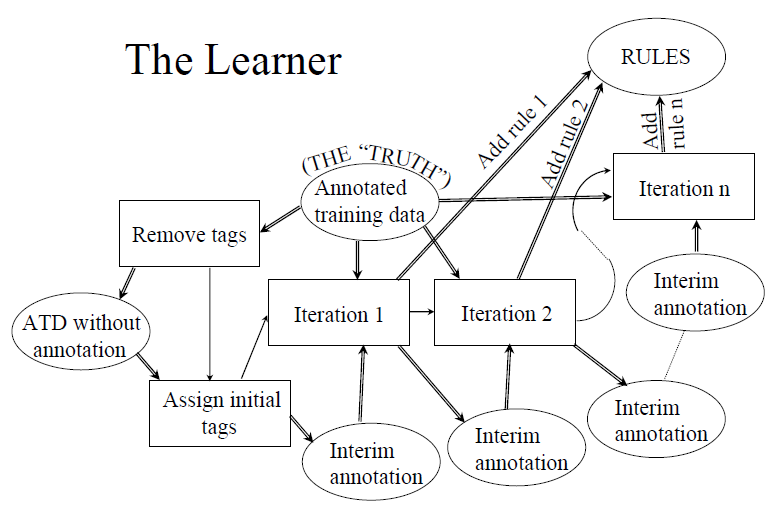
\includegraphics[scale=0.6]{Figures/TBT_learner}
\caption{Learner component of TBT }
\label{fig:tbt_learner}
\end{figure}

\paragraph{The Tagger} The input for tagger is unlabeled data and set of rules $S$ from the learner. Steps for the tagger are straightforward. 
\begin{itemize}
\item Initialize label for lexical items in the same way as the learner did.
\item Loop for all the rules. For each rule \textit{r}, apply this rule to the whole intermediate to change some tag. 
\item The last intermediate data is the output. 
\end{itemize}

TBT is one of the oldest and a very straightforward algorithm, however, it might be used to improve the accuracy of the original tagger. That is, use the original tagger to initialize the learner. \namecite{vietnameseTagger} initialize the learner by using an available English tagger. They also exploit external information from Vietnamese-English parallel data. The English tagger's performance is significantly improved, accuracy improved from 95.4\% to 97.5\% (absolute). 

The Brill Tagger \cite{Brill95transformation} is one of the implementation of transformation base learning. TBT is straightforward but, the learning and tagging is quite slow. Performance of TBT largely depends on having pool of rule templates which are developed by linguist or acquired from machine learning algorithm on annotated corpus. Moreover, compared with other taggers, this approach has rather poorer performance. 

\subsubsection{Hidden Markov Model - a probabilistic approach}
The idea of Hidden Markov Model (HMM) tagger is very similar to noisy channel or translation model in statistical machine translation. The difference is that the output is not a target text but a sequence of tags. Given a sentence which is a sequence of words $W = w_1w_2w_3....w_n$, we need to find the corresponding sequence of tags $T = t_1t_2t_3..t_n$ which maximizes the following probability. 

$$ Tags = \operatorname*{arg\,max}_{t_i} \;P(t_1t_2t_3..t_n|w_1w_2w_3....w_n) = \operatorname*{arg\,max}_{T} \;P(T|W)$$
According to Bayes' rules 
$$P(T|W) = \frac{P(W|T) \times P(T)}{ P(W)} $$
Since we're choosing tags, $P(W)$ is not considered, therefore 
$$Tags = \operatorname*{arg\,max}_{T}\; P(T|W) = \operatorname*{arg\,max}_{T}\; P(W|T) \times P(T) $$
where 
$$ P(W|T) \times P(T)=P(w_1w_2..w_n|t_1t_2..t_n) \times P(t_1t_2..t_n)$$
According to chain rule
$$ P(W|T) \times P(T) = P(w_1|t_1t_2..t_n)\times P(w_2|t_1t_2..t_n) \times P(w_3|t_1t_2..t_n) \times .... \times P(w_n|t_1t_2..t_n) \times $$
$$ P(t_n|t_1..t_{n-1}) \times P(t_{n-1}|t_1..t_{n-2}) \times ...\times P(t_1) $$
\begin{equation}
\label{equa:chainRule}
= \prod_{i=1}^{n} P(w_i|w_1t_1....w_{i-1}t_{i-1}) \times P(t_i|w_1t_1....w_{i-1}t_{i-1})
\end{equation}
With the assumption that the probability of word doesn't depend on the context but only on current tag, we have: 
\begin{equation}
\label{equa:assump1}
P(w_i|w_1t_1....w_{i-1}t_{i-1})  \approx P(w_i|t_i)
\end{equation}
With the assumption that the choice of tag depends on limited history (for example bigram context), we have: 
\begin{equation}
\label{equa:assump2}
P(t_i|w_1t_1....w_{i-1}t_{i-1}) \approx P(t_i|t_{i-1})
\end{equation}
From equation (\ref{equa:chainRule}), (\ref{equa:assump1}) and (\ref{equa:assump2}):
\begin{equation}
\label{equa:hmmFinalEquation}
Tag\; Sequence = \operatorname*{arg\,max}_{T} \; P(W|T) \times P(T) \approx \operatorname*{arg\,max}_{t_i} \; \prod_{i=1}^{n} P(w_i|t_i) \times P(t_i|t_{i-1})
\end{equation}

\begin{figure}
\centering
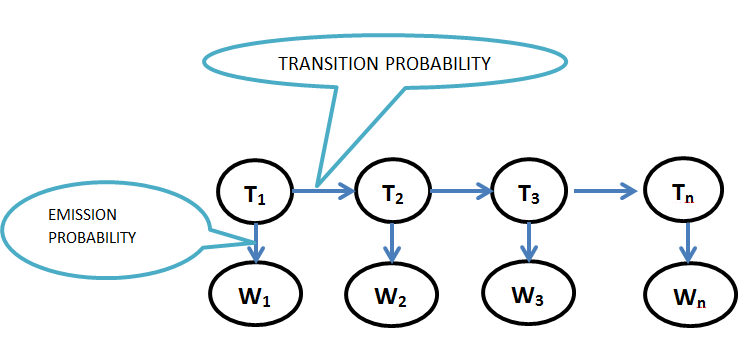
\includegraphics[scale=0.5]{Figures/HMM_tagger}
\caption{Emission and transition probabilities. $W_i$ is a word and $T_i$ is a tag}
\label{fig:hmmTagger}
\end{figure}

$ P(w_i|t_i) $ is called the \textit{emission probability} and $P(t_i|t_{i-1})$ is called the \textit{transition probability} as shown in Figure \ref{fig:hmmTagger}. We estimate these probabilities from training data and then smooth them using method such as interpolation~\cite{REINSCH1967} or Good Turing~\cite{Gale94goodturing}. Smoothing is needed because training data might not cover everything that appears in test data. 

HMM tagging is not as trivial as transformation based tagging. The straightforward tagging solution is that we list all possible tag sequences and calculate the probability of each sequence based on equation \ref{equa:hmmFinalEquation}. The result is the tag sequence that gave the highest probability. However, this solution is not realistic because of the exponential complexity. Therefore, people use dynamic programming algorithms such as Viterbi~\cite{Ryan:1993} or beam search~\cite{beamsearch}.

TNT~\cite{TNTTagger} is an implementation of HMM approach which uses trigram tag model, i.e. $P(t_i|t_{i-1}t_{i-2})$ instead of bigram tag model as mentioned above. Back to Table \ref{tab:eng_state_of_the_art} (page \pageref{tab:eng_state_of_the_art}) , we can see that TNT performs well and achieves comparable result with the state-of-the-art tagger.

\subsubsection{Maximum Entropy - a feature based approach}
We aim at maximizing the following probability 
$$ \operatorname*{arg\,max}_{t_i} \;P(t_1t_2t_3..t_n|w_1w_2w_3....w_n) = \operatorname*{arg\,max}_{T} \;P(T|W)$$
HMM tried to maximize the joint probability $P(W,T)$
$$ \operatorname*{arg\,max}_{T} \;P(T|W) = \operatorname*{arg\,max}_{T} \;P(W|T) \times P (T) = \operatorname*{arg\,max}_{T} \;P(W,T) $$
Maximum Entropy Tagging (MaxEnt)~\cite{maximumEntropy} directly targets maximizing conditional probability $P(T|W)$. 
The disadvantage of HMM tagging is that it cannot incorporate many source of evidence from the text. It just uses lexical and tag information which denoting in emission and transition probability. The MaxEnt model resolves this disadvantage. We can embed as much information as we want in to this MaxEnt model. These information might vary from position, lexical, tag, global document and so forth. Each of these pieces of information are call features. This is the reason why Maximum Entropy tagger belongs to the feature based approach. Formally, a feature is defined as: 

\[
 f_i(C,t) =
  \begin{cases}
   1 & \text{if } context\; C\;is\; satisfied   \\
   0  & otherwise
  \end{cases}
\]

The feature could be complicated or simple, but a feature always in the form, context $C$ and tag $t$. For example a feature ``\textit{suffix = -ing and tag =  VBG}" can be denoted as 
\[
 f_i(C,t) =
  \begin{cases}
   1 & \text{if } \;suffix = \; -ing \; \& \; t = VBG   \\
   0  & otherwise
  \end{cases}
\]\\
The model using these features has to obey the \textbf{constraints}, that is, expected value of feature $f_i$ which is $E_p f_i$ must comply with training data. 
$$E_p f_i = E_{p'}f_i$$
Where 
$$E_{p'}f_i = \frac{1}{N} \sum_{j=1}^{N}f_i(C_j,t_j)$$
$E_{p'}f_i$ is the expected value of feature $f_i$ which is derived from training data ($C_1,t_1$),($C_2,t_2$) .. ($C_n,t_n$). This list can be derived easily from manually annotated data. Apply Lagrangian Multipliers on these constraints, we derived MaxEnt model which has the form as follows:
\begin{equation}
\label{equa:loglinearMaxEnt}
p(t|C) = \frac{1}{Z(C)} exp\Big( \sum_{i=1}^{n}\lambda_if_i(C,t)    \Big)
\end{equation}
Where 
\begin{itemize}
\item $f_i$ is a feature function as defined above 
\item $C$ is the context, t is tag 
\item $Z(C)$ is the normalization factor to ensure proper distribution probability. 
\item $\lambda_i$ is the weight for features $f_i$
\end{itemize}
The more common name for this model is ``log-linear model". We use Generalized Iterative Scaling (GIS)~\cite{Darroch1972} to estimate $\lambda_i$. The value of  $\lambda_i$ shows the importance of feature $f_i$. This value has to obey the \emph{constraints} applied for feature $f_i$. The GIS algorithm is shown in Algorithm \ref{alg:findLambda}.
\begin{algorithm}
\caption{Finding $\lambda_i$}
\label{alg:findLambda}
\begin{algorithmic} 
\STATE $\lambda_i^{(0)} \leftarrow 0$
\WHILE{$not\;convergence$}
\STATE $C \leftarrow max_{C,t} \sum_{i=1}^{n} f_i(C,t)$
\STATE $\lambda_i^{(t+1)} \leftarrow \lambda_i^t + \frac{1}{C}log\frac{E_{p'}f_i}{E_{p^{(t)}}f_i}$
\ENDWHILE
\end{algorithmic}
\end{algorithm}

It is very important to notice that the constraints cannot uniquely define the model in Equation (\ref{equa:loglinearMaxEnt}). So, from all models that satisfy constraints, we choose a model that \textit{maximizes entropy}, that is, as uniform as possible. Moreover, tag probability truly depends on the context which is described by features, therefore: 
\begin{equation}
\label{equa:finalMaxEnt}
Tag\; Sequence = \operatorname*{arg\,max}_{T} \;P(T|W) = \operatorname*{arg\,max}_{T}; P(T|C) \approx \operatorname*{arg\,max}_{t_i};\prod_{i=1}^{n} p(t_i|C_i)
\end{equation}
Finally, the most probable sequence of tags (\textit{result tag sequence}) is obtained by performing beam search~\cite{beamsearch} or Viterbi~\cite{Ryan:1993} algorithms to maximize equation (\ref{equa:finalMaxEnt}). 

The most common implementation of MaxEnt tagger uses features from two words back and ahead, the current word, and two tags back. That is, context C = $(w_{i-2},t_{i-2}, w_{i-1}, t_{i-1}, w_i, w_{i+1}, w_{i+2})$. Features can be anything from this context. Therefore, the number of features can be numerous and degrade the performance. Effective implementation always uses some heuristic methods to limit the number of features. Stanford Maximum Entropy tagger~\cite{Toutanova:2003} is one of notable such implementation. From Table \ref{tab:eng_state_of_the_art} (page \pageref{tab:eng_state_of_the_art}), we can see that aside from Stanford MaxEnt, there are many other systems i.e. GENiA Tagger~\cite{Toutanova03} or Maxent easiest-first~\cite{Tsuruoka:2005}  exploit MaxEnt idea and acquire very good result. This is somehow understandable because MaxEnt has the power to incorporate all features. In that way, we capture all evidence that could help to predict tags.  
% How to construct features .

\subsubsection{Other algorithms}
Apart from the above mentioned approaches (rule based, probabilistic, feature based), there are other approaches for supervised POS taggers. 

The \textit{classifier base approach} is one of those. They build a classifier based on machine learning algorithms such as Naive Bayes, Decision Tree, kNN or more advanced methods: Support Vector Machines (SVM) or Conditional Random Fields (CRF) and so forth. Each lexical item (word) is converted into features, then a classifier is  trained on this data. The test data is also converted into features. We run the classifier on test data and produce tag labels. Steps for classifier approach are described in Figure \ref{fig:machineLearning}. Back to Table \ref{tab:eng_state_of_the_art} (page \pageref{tab:eng_state_of_the_art}), SVMtool~\cite{svmtool} implement SVM machine learning algorithm performs very well on Wall Street Journal (WSJ) data set.
\begin{figure}
\centering
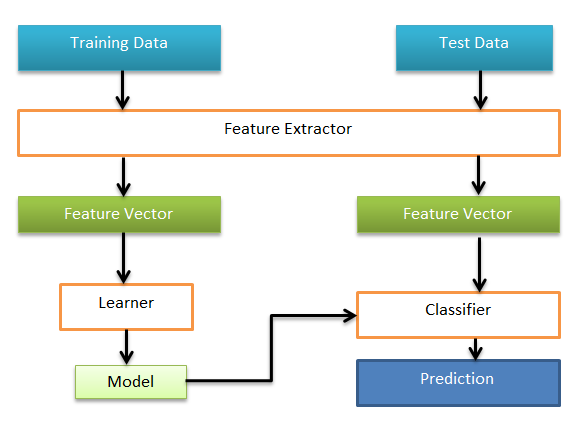
\includegraphics[scale=0.6]{Figures/MachineLearning}
\caption{Steps to build a classifier}
\label{fig:machineLearning}
\end{figure}

\textit{Parsing approach} exploits the idea of building a constituency parse tree as in Figure \ref{fig:parsingTagging}. Afterward, we need to track down the rules to determine tags. For example, from rule NP $\rightarrow$ DT NN, we extract ``\textit{a}" (DT) and ``\textit{fly}" (NN). However, parsing task is more difficult than tagging and actually uses information from tagging processes. Nevertheless, parsing could be very helpful for tagging especially in the case where disambiguation needs a long range syntactic information as in Chinese or Japanese. Traditionally, a constituency parser is built from a tree bank using algorithms such as shift-reduce parsing \cite{shiftReduce}. Modern approach does POS tagging and parsing at the same time in an incremental way \cite{ParsingAndTagging}. 
\begin{figure}
\centering
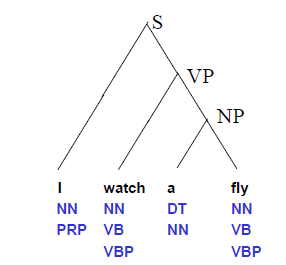
\includegraphics[scale=0.8]{Figures/Constituency_parsing}
\caption{Constituency Parse Tree}
\label{fig:parsingTagging}
\end{figure}

\subsection{Unsupervised}
Unsupervised tagging does not use any labeled data for training. There are several well-known methods for unsupervised tagging.  
\subsubsection{Clustering}
Words having the same syntactic properties are grouped into the same group (cluster). It is believed that words in the same cluster are likely to have the same POS tag. The first issue a clustering tagger has to tackle is \textit{measuring syntactic similarity}. That is if each word is a vertex in a graph, and the weight of edges between vertexes is the syntactic similarity, then words which have the same POS label must be close to each other. Normally, similarity measurement algorithm is based on nearby content words. For example, in two sentences ``\textit{He bought a pair of shoes}" and ``\textit{He ate a banana}". Two words ``\textit{bought}" and ``\textit{ate}" are surrounded by ``\textit{He}" and ``\textit{a}", therefore ``\textit{buy}" and ``\textit{eat}" are likely to have the same POS tag. \namecite{disPOSTagging} proposes to use distributional similarity for measurement. This approach is based on the hypothesis that, ``we can understand a word by looking at its neighbor feature words". Afterward, a word is displayed as vectors of feature words. To compensate for the frequency effects, the weight for each feature word is calculated using a method such as tf.idf~\cite{tfidf}. \namecite{disPOSTagging} considers the top $n$ most frequent words as feature words. A word is displayed as: 
$$\overrightarrow{word A} = (w_1,w_2,w_3......w_n)$$
where $w_i$ is the weight of the $i^{th}$ feature word and $w_i$ = 0 if that feature word does not appear in the context of current $word A$. The similarity between two words is the cosine similarity between the corresponding vectors. 

Another problem with clustering tagger is \textbf{determining the number of clusters}. Defining that number beforehand might not be a good solution. We might force the algorithm to separate coherent cluster or to join unrelated one. On the other hand, letting the algorithm choose when to stop could result in a too specific or too general cluster. 

\textbf{Evaluation} is also another major consideration. Normally, clustering algorithms are evaluated based on the perplexity (or entropy) of the cluster. In the case of tagging, we are expecting that all words in the same cluster have the same tag. Therefore, the lower the perplexity, the better. However, is it what we are looking for? The answer is no, we want to compare with gold standard test data to know the tagging performance. \citeauthor{ManyToOneEvaluate} (2007) suggested a \textit{many-to-one} evaluation. The induced tag for each cluster is the most frequent tag of the items in the cluster, consulting the gold standard data. However, there are cases where two clusters have the same tag. To resolve this issue,\textit{ one-to-one} evaluation puts the restriction that each gold tag corresponds to only one cluster. Normally, it is done by greedy matching, which aims at maximizing  accuracy. Nevertheless, the number of clusters and gold tags are likely to be different. In that case, some clusters or gold tags will not be matched. However, both \textit{many-to-one} and \textit{one-to-one} evaluation schemes require gold data to find the most appropriate tag for each cluster. This is a chicken-and-egg problem since if we have gold data then we don't need to take an unsupervised approach. Besides, we can also use some heuristic method to determine the tag for each cluster such as cluster size (eg, the biggest cluster is Noun). 

UnsuPOS\footnote{http://wortschatz.uni-leipzig.de/\textasciitilde cbiemann/software/unsupos.html} \cite{unSupPOSClustering} is an implementation of a clustering tagger. He divides words into two partitions: high and medium frequency words, medium and low frequency words. In each partition, he builds a different graph using a different similarity measurement. For high and medium frequency words, he uses distributional similarity as mentioned above. For the other partition, he calculates similarity between two words based on how many \textit{direct} neighbors they have in common. The edge is made between words (vertex) if the weight is higher than a threshold. Afterward, the Chinese Whispers~\cite{chineseWhisper} clustering algorithm is performed on both graphs. Steps for Chinese Whispers are simply as follows: (1)~each node is assigned to a cluster; (2)~sort the nodes in an random order; (3)~join node to it most popular neighborhood where popularity is defined as the total weight of inside nodes; (4)~repeat (3) until the number of cluster reaches the fix point. 


Thereafter, on each partition, there is a set of clusters. It is worth noticing that there are many words in common (medium frequency words) between clusters. Then, \namecite{unSupPOSClustering} merges these two sets into a single set. Again, each cluster is considered as a vertex and the number of common words is the weight between vertexes. Chinese Whisper is applied  again to acquire final clusters. Every word inside a cluster has cluster ID as the tag label. Finally, he build a tagging model using a trigram HMM. 

Unsupervised tagging using a clustering algorithm is useful since it provides the first overview about syntactic categories of lexical items. In reality, it is usually used with other applications, for example, \namecite{semiSuPOSCondense} uses unsupervised tagging information as the feature to build another tagger. 

\subsubsection{HMM unsupervised tagging}
\label{hmmUnsup}
In a supervised HMM tagger, we estimate emission probability $p(w_i|t_i)$ and transition probability $p(t_i|history)$ from the labeled training data. In the unsupervised style, these two probabilities are estimated using the Baum-Welch~\cite{BaumWelch} algorithm, which is a variant of the \textit{Expectation Maximization (EM)} algorithm. It means that Baun-Welch can only output the local best but not the global optimal solution. Baum-Welch makes use of forward and backward algorithms~\cite{forwardBackward}. It uses the sequence of observations and outputs the most likely parameters (emission and transition probability) for the HMM. Roughly speaking, the steps for Baum-Welch are described in Algorithm \ref{alg:baumWelch}. 
% Steps for baun-welch 
\begin{algorithm}
\caption{Baum-Welch algorithm}
\label{alg:baumWelch}
\begin{algorithmic} 
\STATE Initialize emission probability $P_Y$
\STATE Initialize transition probability$P_S$
\WHILE{$not\;convergence$}
\STATE {Compute forward probability } 
\STATE (1) Using current setting of $P_S$ and $P_Y$
\STATE (2) Follow the procedure of trellis algorithms  

\STATE {Compute backward probability } 
\STATE (1) Same as forward probability
\STATE (2) Start from the end 

\FOR {each emission/transition pair}
\STATE {Collect count base on forward \& backward prob}
\ENDFOR

\STATE {Re-estimate $P_S$ and $P_Y$}
\ENDWHILE
\end{algorithmic}
\end{algorithm}

\textit{Feature based HMM} (FB-HMM) \cite{featurebaseHMM} is another variance of unsupervised HMM tagging. The emission probability model $P(w_i|t_i)$ is estimated using a log-linear model:
$$P(w_i|t_i) = \frac{exp(weight \times f(w_i,t_i)}{\sum_{x' \in Voc} exp (weight \times f(x,t_i))}$$
where $Voc$ is the entire vocabulary and $f(w_i,t_i)$ is the feature as in supervised feature based learning. Again, this model can incorporate many source of evidence from the observation $w_i$. In the original paper, \namecite{featurebaseHMM} use features including: (1)~original word $w_i$; (2)~whether $w_i$ contains digit or not; (3)~whether $w_i$ contains a hyphen or not; (4)~whether the first character is capital or not and (5)~the features from the previous 3 words. The feature based HMM performed better than EM-HMM, simply because it exploits more information. Table \ref{tab:superviseUnsupervise} show the margins of 6.3 \% (absolute) in average accuracy between FB-HMM (73\%) and EM-HMM (66.7\%).

\begin{table}
\tiny
  \centering
%	\tabsep0pt
    \begin{tabular}{lp{2cm}|cccccccc|c}
    
    &Model & da & nl & de & el & it & pt & es & sv & \textbf{Avg} \\
    \hline

    \multirow{2}{*}{Without dic.} & EM-HMM  & 68.7  & 57    & 75.9  & 65.8  & 63.7  & 62.9  & 71.5  & 68.4  & 66.7 \\

    & FB-HMM &69.1& 65.1 &81.3 &71.8 &68.1& 78.4& 80.2 &70.1 &73.0\\
    \hline
    With dic. & FB-HMM & 93.1  & 94.7  & 93.5  & 96.6  & 96.4  & 94    & 95.8  & 85.5  & 93.7 \\
    \end{tabular}
  \caption{Comparison between with and without dictionary unsupervised POS tagger for 8 languages (Danish(da), Dutch(nl), German(de), Greek(el), Italian(it), Portuguese(pt), Spanish(es), Swedish(sv) }  
  \label{tab:superviseUnsupervise}
\end{table}


In the unsupervised HMM approach, we assume that we know the tag set and \textit{possible tags for each word}. We can get this list of possible tags from the dictionary or from training data. If we don't have this resource, the system would be completely unsupervised. However, without this list, the performance would degrade substantially. \namecite{Das:2011} use the same tagset for different languages, the comparison of supervised, completely unsupervised (without dictionary EM-HMM and FB-HMM), and unsupervised with dictionary (with dictionary FB-HMM) tagger are given in Table \ref{tab:superviseUnsupervise}. The effectiveness of the gold dictionary is clearly visible. The average accuracy increases from 73.0\% to 93.7\% (absolute). 

\subsection{Semi-supervised}
Semi-supervised learning is the combination of supervised and unsupervised method. The amount of labeled data is not enough to build a reliable supervised system. On the other hand, unlabeled data is widely available and easy to access in large quantity. In this circumstance, semi-supervised learning is the solution. Moreover, even in the case where labeled data is big enough, combining with unlabeled data might give better performance. 

\subsubsection{Self-training, Tri-training approach}
The most straightforward approach to semi-supervised tagging is self-training. That is, we train a supervised classifier $c$ from labeled data $L$. This model is used to label unlabeled data $U$, so $U$ will become labeled data $L'$. Afterward, we merge $L'$ and the gold labeled data $L$, and train new classifier $c'$ on them. The process is repeated until no new classifier is constructed. Tri-training~\cite{triTraining} is the extension of self-training. Instead of using just one classifier, tri-training uses three classifiers. All three classifiers are originally trained on \textit{bootstrapped} gold data. Bootstrapping is a technique for re-sampling the data. It is very important to use bootstrapped data, because if training data for three classifiers is not diverse, the three classifiers would be the same and tri-training would become self-training. When labeling a data item from unlabeled data $U$, two classifiers would help to determine the label. The intuition here is that when two classifiers agree upon a label, it is likely to be correct. The algorithms stop when no new classifiers are built. The detailed steps are described in Algorithm \ref{alg:triTraining}. 
% Steps for tri-training 
\begin{algorithm}
\caption{Tri-training algorithm}
\label{alg:triTraining}
\begin{algorithmic}[1] 
\STATE $L_i \leftarrow bootstrap(L) $ : i = 1..3
\STATE $c_i \leftarrow train\_classifier(L_i)$ : i = 1..3
\REPEAT
\FOR {i : 1..3}
\FOR { $x \in Unlabeled\; data$ } 
	\IF {$c_j(x) = c_k(x)\; \& \; (j,k:1..3)\; \& \;(j,k \neq i) $} 
	\STATE $L_i \leftarrow L_i \cup (x,c_j(x))$		
	\ENDIF
\ENDFOR
\STATE $c_i \leftarrow train\_classifier(L_i)$ : i = 1..3
\ENDFOR
\UNTIL{$c_i$ not change}
\STATE $Final\; classifier \leftarrow vote\; of\; c_i $ : i= 1..3
\end{algorithmic}
\end{algorithm}

\namecite{semiSimple} suggested a simple improvement for tri-training, that is, tri-training with disagreement. He just simply replaced the condition {$ if \;c_j(x) = c_k(x)$} (in line 6, Algorithm \ref{alg:triTraining}) with condition, $ if \;c_j(x) = c_k(x)\neq c_i(x)$. The accuracy and especially \textbf{speed} improved. It might be because the new condition just focuses on the weak point of the classifier. The advantage of self-training is the method's simplicity. However, in practice, without exploiting extra information, self-training gives very little improvement. Table \ref{tab:triTraining} shows the result of self-training, tri-training and tri-training with disagreement on the same WSJ data set based on the two tagger SVM Tool~\cite{svmtool} and MaxEnt~\cite{Toutanova:2003}. Tri-training with disagreement performs exactly the same as Tri-training on both models. However, due to the modification in the condition, Tri-training with disagreement runs faster. The improvement of Tri-training over self-training is not clearly visible. 
\begin{table}
\;
  \centering
    \begin{tabular}{p{2cm}|cccc}
    & Original & Self-training & Tri-training & Tri-training with dis.\\
    \hline
	SVM Tool & 97.15 & 97.26 & 97.27 & 97.27 \\
    \hline
	MaxEnt & 96.31 & 96.36 & 96.36 & 96.36 \\
    \hline
    \end{tabular}
  \caption{Comparing self-training, tri-training and tri-training with
   disagreement}  
  \label{tab:triTraining}
\end{table}
\subsubsection{Semi-supervised condensed nearest neighbor}
Looking back at Table \ref{tab:eng_state_of_the_art} (page \pageref{tab:eng_state_of_the_art}), the semi-supervised condensed nearest neighbor (SCCN) tagger \cite{semiSuPOSCondense} gave the highest accuracy (97.5\%) on the WSJ data set. \namecite{semiSuPOSCondense} exploited the vast amount of unlabeled data to find a better center point for each cluster. SCCN is based on the kNN machine learning algorithm. That is, the label is chosen based on the vote of k nearest neighbors. Similarity measurement between data points are first to be put into consideration. Each data point is translated into a vector $ \overrightarrow{x} = (m,n)$, where $m$ is the label given by the supervised tagger SVMTool~\cite{svmtool} and $n$ is the label/clusterID given by unsupervised clustering tagger UnSuPos~\cite{unSupPOSClustering}. Examples of data points for training are given in Table \ref{tab:sampleDataPoin}. 
\begin{table}
  \centering
    \begin{tabular}{p{4cm}|p{4cm}p{4cm}}
     Gold Label & Supervised label & Unsupervised label \\\hline
     NN & NN & 14 \\\hline
     VB & VBZ & 121 \\\hline        
     DET & DET & 11 \\             
     ... & ... & ...\\             
    \end{tabular}

  \caption{Sample data point in train data}  
  \label{tab:sampleDataPoin}
\end{table}
The similarity between two data points is calculated based on euclidean distance between two corresponding vectors. 

kNN is considered as a lazy method as it does not actually build a model. Every time, it needs to scan through all the data points again. Therefore, the complexity of kNN for each tag is proportional to the number of labeled data points. In this way, it is not possible for kNN to run on big data sets. The condensed nearest neighbor (CNN)~\cite{semiSuPOSCondense} is an intuitive solution. CNN tries to condense the data by filtering out data points which are not a good representation. The condense technique is straightforward, as shown in Algorithm \ref{alg:condenseNN}. $L$ is the labeled data points, where $x_i$ is data and $y_i$ is the tag. The initial $classifier$ is trained on $L$. \namecite{semiSuPOSCondense} uses this classifier to discard all the data points that are correctly tagged. An extension of CNN is weakened condensed nearest neighbor (WCNN) where they just discard any high confidence correctly classified items. It means that line 4 of Algorithm \ref{alg:condenseNN} will be replaced by \textbf{if} $Classifier(x_i) \neq y_i \; or \; Prob(x_i,y_i) < threshold$. where $Prob(x_i,y_i)$ denotes the classifier confidence. 
\begin{algorithm}
\caption{Condense Nearest Neighbor algorithm}
\label{alg:condenseNN}
\begin{algorithmic} [1]
\STATE $L = \{(x_1,y_1),(x_2,y_2) .... (x_n,y_n)\} $ 
\STATE $C \leftarrow \{\}$
\FOR { $(x_i,y_i) \in L$ }
	\IF {$Classifier(x_i) \neq y_i$} 
	\STATE $C \leftarrow C \cup (x_i,y_i)$		
	\ENDIF
\ENDFOR
\end{algorithmic}
\end{algorithm}
Basically, CNN or WCNN tries to find the best representative points for each cluster. Ideally, each cluster will find one and just one single point located at the center of cluster. However, since the amount of labeled training data is not big enough, it is unlikely to cover this point. This is exactly where \textbf{unlabeled data comes into play}, with the advantages of gigantic size, it is high chance that unlabeled data points would be close enough to the center point. Semi-supervised weakened condensed nearest neighbor is described in Algorithm \ref{alg:semiSupcondenseNN}. Firstly, they obtain condensed data points $C$ using WCCN. For each unlabeled data item, they try to tag it using $C$. If it is tagged with high confidence (greater than some threshold, i.e.\ 0.9), they add this point and its label to $C$. In the last step, they apply the condense technique again on $C$ to get final condensed set of data points $C'$. Using $C'$ to tag is as trivial as in any kNN algorithms. For the WSJ dataset, this method actually gave the highest accuracym 97.5\%. Moreover, it also runs extremely quickly thanks to very small number of data point in $C'$. \namecite{semiSuPOSCondense} pointed out that it condenses the 1.2 million data points of the Brown Corpus to just 2249 items. 
\begin{algorithm}
\caption{Semi-Supervised Weakened Condense Nearest Neighbor algorithm}
\label{alg:semiSupcondenseNN}
\begin{algorithmic} [1]
\STATE $L = \{(x_1,y_1),(x_2,y_2) .... (x_n,y_n)\} $ 
\STATE $U = \{(x'_1),(x'_2), .... (x'_m)\}$
\STATE $C \leftarrow WCNN(L)$
\FOR { $(x'_i) \in U$ }
	\IF {$TagProb(x'_i) > threshold $} 
	\STATE $C \leftarrow C \cup (x'_i,y'_i)$		
	\ENDIF
\ENDFOR
\STATE $C' \leftarrow WCNN(C)$
\end{algorithmic}
\end{algorithm}

\section{Multilingual POS Tagger}
This section reviews methods for creating taggers for multiple languages based on parallel/comparable data. Comparable documents contain the \emph{rough} translation of each other, for example, Wikipedia documents for different languages are comparable. \namecite{YarowskyAndNgai}, \namecite{XiAndHua}, \namecite{SnyderMultilingualPOS} and \namecite{Das:2011} exploit this idea. The following is the overview of their approaches. 

\subsection{Typologically related languages approach}
This approach restricts to very closely related language such as Czech and Russian, Telugu and Kannada and so forth. \namecite{Hana04}, \namecite{Feldman06}, \namecite{reddy2011crosspos} have exploited this idea. HMM taggers need emission probabilities and transition probabilities. The intuition here is that if two languages are typologically related, \textbf{their transition probabilities would be very similar}, that is, the tag sequences between these languages are similar to each other. Therefore, we can use transition probability interchangeably. \namecite{reddy2011crosspos} built a tagger for Kannada from Telugu. Kannada and Telugu are both spoken in India by 35 million and 70 million people respectively. Telugu are more widely spoken and has better resources. Steps to construct Kannada tagger is as follows: 
\begin{enumerate}
\setlength{\itemsep}{0pt}
\item Collect large corpora for Kannada and Telugu 
\item Tag the Telugu side using the available tagger
\item Calculate the Telugu transition probabilities $p(t_i|t_{i-1},t_{i-2})$
\item Estimate Kannada emission probabilities $p(w_i|t_i)$
\item Build Kannada tagger from steps 3 and 4
\end{enumerate}

It is worth noticing that this method does not need to collect parallel data of Kannada and Telugu. Monolingual or comparable corpora would work in this case. Hence, \namecite{reddy2011crosspos} used Corpus Factory~\cite{CorpusFactory} to crawl monolingual data from the internet. Telugu has POS manually annotated data. Therefore, constructing a tagger, tagging and calculating transition probability (Step 2 and 3) is not a problem. However, step 4 is not trivial. The first solution is that, we can also estimate Kannada emission probability $p_K(w_i|t_i)$ via Telugu emission probability $p_T(w'_i|t_i)$ where $w'_i$ and $w_i$ are very similar to each other. Kannada and Telugu are very closely related languages, therefore, they share many lexical item in common. It is possible to find the closest word $w'_i$ of $w_i$ using any approximate string matching (fuzzy matching). \namecite{reddy2011crosspos} also suggested using uniform distribution of all possible tags for emission probability. For each words, they get the list of possible tags from dictionary, and then assume that the tags are distributed uniformly. This turn out to be quite effective. Table \ref{tab:topologyRelatedLang} shows some results. The emission probability of model 1 is based on string approximation. It gave an encouraging result since they actually did not use any resource aside from monolingual data. Model 2 is surprisingly high. However, model 2 use gold dictionary to look for possible tags of each words which is hard to acquire. Model 3 uses actual emission probabilities from the target language. That is, we estimate emission probabilities using a supervised target language (Kannada) tagger. Model 3 is added for comparison purposes only. Model 4 is more or less the upper bound that the other models can get. Transition and emission probabilities are estimated directly from the Kannada side (using supervised tagger). Remarkably, model 3 and 4 gave very close result. This consolidates the hypothesis that ``for closely related languages, transition probability are interchangeable".
\begin{table}
  \centering
    \begin{tabular}{c|llc}
    \textbf{Model} & \textbf{Transition Prob.}& \textbf{Emission Prob.} & \textbf{F-measure} \\
	\hline
	1 & From source language & Approximate string matching & 56.88 \\
	2 & From source language & Uniform distribution target tags & 75.10 \\
	3 & From source language & Target language emission Prob. & 77.63 \\	
	4 & From target language & Target language emission Prob. & 77.66 \\		
    \end{tabular}%
 \caption{Various tagging model exploit topologically related language}
  \label{tab:topologyRelatedLang}%
\end{table}%

\subsection{Unsupervised simultaneously tagging approach}
A previous approach used typologically related languages. It assumed the presence of tagger or labeled data of a source language and then copied transition probabilities to the target language. This approach, however, does not need any labeled data in both languages, words are tagged \textbf{simultaneously} \cite{SnyderMultilingualPOS}. Firstly, alignment are run to align words for each sentences. Word alignment exploits IBM models (1..5) and will be trained on large amount of parallel data. The output of the aligner is the list of mappings between words from source and target sentence going with confidence. We discard low confidence, cross-edges and multiple mapping. So, the remaining is high confidence one-to-one word alignment. These word pairs would be the observation of the model. Thus, for each sentence pair, just some words are aligned and the rest (the major) is unaligned. They try to maximize the following probability given the observed alignment and words. 

\begin{dmath}
P(x_1,x_2...x_m, y_1,y_2..y_n | a, \phi, \phi',w) = \prod_{unaligned\;i} \phi_{x_{i-1}}(x_i)  \times  \prod_{unaligned\; j}\phi'_{y_{i-1}}(y_j) \times \prod_{(i,j)\in a} P(x_i,y_j|x_{i-1},y_{j-1},\phi,\phi',w)
\label{equa:simulTagging}
\end{dmath}
where $x_1,x_2...x_m$ is a tag sequence of the source language, $y_1,y_2..y_n $ is a tag sequence of the target language, $a$ is the alignment, $\phi$ and $\phi'$ are transition probabilities of source and target language respectively; and $w$ is the bilingual coupling distribution $w : T \times T'$ where $T$ and $T'$ are tag sets of the two languages. They infer equation (\ref{equa:simulTagging}) using Gibbs Sampling. They sample (1) the tag sequence $(x_i,y_j)$, (2) monolingual transition probability $\phi$ and $\phi'$, (3) coupling distribution $w$ and then integrate over emission probabilities. The model is evaluated on 4 languages: English, Bulgarian, Slovene and Serbian. The baseline for each language is calculated using a monolingual unsupervised HMM with gold dictionary. That is, possible tags for each word are provided. Table \ref{tab:simultaneouslyTagging} shows the constant improvement of bilingual simultaneous tagging over monolingual tagging. Of particular note, tagging accuracy of Slovene improves 7.69\% when paired with Serbian which is very closely related language, but only 1.3\% when going with English. Thus, we can see that choosing the right language pair would significantly improve the performance. 
\begin{table}
  \centering
    \begin{tabular}{r|ccc}

          & \textbf{Monolingual} & \textbf{Simultaneously} & \textbf{Improvement} \\
	\hline
    EN    & 90.71 & 91.01 & +0.3 \\
    SR    & 85.05 & 90.06 & +5.03 \\
    \hline
    EN    & 90.71 & 92    & +1.29 \\
    BG    & 88.88 & 94.48 & +5.61 \\
    \hline
    EN    & 90.71 & 92.01 & +1.3 \\
    SL    & 87.41 & 88.54 & +1.13 \\
    \hline
    SL    & 87.41 & 95.1  & +7.69 \\
    SR    & 85.05 & 91.75 & +6.7 \\
    \hline
    BG    & 88.88 & 91.95 & +3.08 \\
    SR    & 85.05 & 86.58 & +1.53 \\
    \hline
    BG    & 88.88 & 90.91 & +2.04 \\
    SL    & 87.41 & 88.2  & +0.79 \\

    \end{tabular}
  \caption{Per-token tagger accuracy with gold dictionary for unsupervised monolingual and bilingual simultaneously tagging}    
  \label{tab:simultaneouslyTagging}%
\end{table}%

\begin{table}
  \centering
    \begin{tabular}{r|ccc}

          & \textbf{Monolingual} & \textbf{Simultaneously} & \textbf{Improvement} \\
	\hline
    EN    & 63.57 & 68.22 & +4.66 \\
    SR    & 41.14 & 54.73 & \textbf{+13.59} \\
    	\hline
    EN    & 63.57 & 71.34 & +7.78 \\
    BG    & 53.19 & 62.55 & \textbf{+9.37} \\
    	\hline
    EN    & 63.57 & 66.48 & +2.91 \\
    SL    & 49.9  & 53.77 & +3.88 \\
    	\hline
    SL    & 49.9  & 59.68 & \textbf{+9.78} \\
    SR    & 41.14 & 54.08 & \textbf{+12.94} \\
    	\hline
    BG    & 53.19 & 54.22 & +1.04 \\
    SR    & 41.14 & 56.91 & \textbf{+15.77} \\
    	\hline
    BG    & 53.19 & 55.88 & +2.7 \\
    SL    & 49.9  & 58.5  & +8.6 \\

    \end{tabular}
  \caption{Per-token accuracy with reduced gold dictionary size for unsupervised monolingual and bilingual simultaneously tagging. Huge improvements are in bold}    
  \label{tab:simultaneouslyTaggingReducedDic}%
\end{table}%

They further reduce the size of the gold dictionary to just the 100 most frequent words. The effectiveness of bilingual tagging is highlighted. Table \ref{tab:simultaneouslyTaggingReducedDic} shows the huge improvement of bilingual simultaneously tagging. This table also highlights the differences in performance when changing the source language. For example, pairing BG with SR improves SR only 1.53\% when full size dictionary is used (Table \ref{tab:simultaneouslyTagging}), however, improve $\approx 16$\% on reduced dictionary (Table \ref{tab:simultaneouslyTaggingReducedDic}). 

\subsection{Tag projection approach}
A number of studies have used \emph{tag projection} to copy tag
information from a resource-rich to resource-poor language, based on
word alignments in a parallel corpus. After alignment, the
resource-rich language is tagged, and tags are projected from the
source language to the target language based on alignment
\cite{YarowskyAndNgai} and \cite{Das:2011}.  \namecite{Das:2011} achieved
the current state-of-the-art for unsupervised tagging by exploiting
high confidence ($>0.9$) alignments to copy tags from the source language to
the target language.  

\begin{table}
\centering
    \begin{tabular}{lc}
    Description               & Features          \\\hline
    Trigram + Context         & $x_1x_2x_3x_4x_5$ \\
    Trigram                   & $x_2x_3x_4$       \\
    Left Context              & $x_1x_2$          \\
    Right Context             & $x_4x_5$          \\
    Center Word               & $x_3$             \\
    Trigram - Center Word     & $x_2x_4$          \\
    Left Word + Right Context & $x_2x_4x_5$       \\
    Left Context + Right Word & $x_1x_2x_4$       \\
    Suffix                    & hasSuffix$(x_3)$  \\
    \end{tabular}
    \caption{Features used for computing similarity between trigram vertex}
    \label{tbl:featuresForSimilarity}
\end{table}
% Graph construction 
Graph-based label propagation was used to automatically produce more labelled training data. First, a graph was constructed in which each vertex corresponds to a unique trigram in the target language, and edge weights represent the syntactic (POS) similarity between two vertices. The syntactic similarity function is calculated from the window of two words around the target words. The features for trigram $x_2x_3x_4$ in the sequence of $x_1x_2x_3x_4x_5$ are described in Table \ref{tbl:featuresForSimilarity}\footnote{hasSuffix($x_3$) feature check the target word $x_3$ has suffix or not}. The idea here is that they expect the same part-of-speech for words used in the same context. For example, two trigrams ``he-has-lunch" and ``he-gets-lunch" share the same $x_2 = he, x_4 = lunch$ therefore, ``has" and ``gets" are likely to have the same POS tag. 

Labels were then propagated by optimizing a convex function to favor
the same tags for closely related nodes while keeping a uniform tag
distribution for unrelated nodes. They extract tag dictionary from the automatically labelled data. This dictionary, in  turn, was used to constrain a
feature-based HMM tagger \cite{featurebaseHMM}.

\namecite{Das:2011}  experimented on 8 languages: Danish(da), Dutch(nl), German(de), Greek(el), Italian(it), Portuguese(pt), Spanish(es), Swedish(sv). They used parallel data from Europarl~\cite{europarl} and the ODS United Nations dataset which has English in the source side. They evaluated target language tagger performance on gold test data mainly from the CoNLL-X and CoNLL 2007 shared tasks. Table \ref{tbl:annotatedData} (page \pageref{tbl:annotatedData}) shows the detailed source and size for each gold test data set. To avoid mapping between different tagsets, they use consensus 12 Universal Tags \cite{UniversalTagSet} across languages. 

\namecite{Das:2011} experimented with 7 different models. 
\begin{enumerate}
\item Unsupervised EM-HMM, which is a traditional expectation maximization unsupervised HMM. EM-HMM is mentioned in section \ref{hmmUnsup} (page \pageref{hmmUnsup}). 

\item Unsupervised Feature based - HMM is another style of unsupervised HMM which is also mentioned in section \ref{hmmUnsup} (page \pageref{hmmUnsup})

\item Direct projection, that is, tags are projected from source language to target language. Unaligned words are tagged with the most frequent tag. Afterward, supervised POS tagging is trained on this data.

\item No label propagation. The dictionary is extracted from direct projected tags. The graph-base label propagation step is not performed. 

\item With label propagation. The full model, dictionary is extracted after label propagation step. 

\item With gold dictionary. Gold dictionary is extracted from annotated data. This dictionary is fed into a feature base-HMM tagger as the constraint. 

\item Supervised, the supervised POS tagger is trained on annotated data.
\end{enumerate}
Model (1), (2), (3) are used as the baseline to compare. Comparing (4) and (5) show the effectiveness of label propagation. Model (6) show the upper bound of this approach. Model (7) is for comparing with supervised method. The performance of each model on 8 languages is described in Table \ref{tab:dasTable}. 

As expected, unsupervised feature based HMM (model 2) performs better than the traditional EM-HMM (model 1). The tagger built on direct projection (model 3) is actually a weakly supervised~\footnote{Unlike supervised, weak supervised (or some time called distant supervised) learning doesn't have the actual gold training data, these data are induced from heuristic step and not completely correct.} system, because the target language labels are not 100\% correct, coming from the heuristic (projection) step. However, it still performs better than the completely unsupervised method, EM-HMM (model 1) and Feature-HMM (model 2). Label propagation (model 5) shows constant improvements over all 8 languages, improved 2\% (absolute) compared with model 4 where label propagation was not employed. This improvement is mainly because performing label propagation enlarges the dictionary size and thus, improves the vocabulary coverage. This full model with Label Propagation (model 5) outperforms unsupervised methods (model 1, 2) and does better than direct projection (model 3) at 7 languages out of 8. It also narrows the gap between unsupervised and supervised methods (model 7). In this thesis, we will mainly compare with this work as it is considered as the state-of-the-art system for unsupervised multilingual POS tagger

\begin{table}[htbp]
  \centering

    \begin{tabular}{l|rrrrrrrr|r}
    \multicolumn{1}{c}{Model} & \multicolumn{1}{c}{da} & \multicolumn{1}{c}{nl} & \multicolumn{1}{c}{de} & \multicolumn{1}{c}{el} & \multicolumn{1}{c}{it} & \multicolumn{1}{c}{pt} & \multicolumn{1}{c}{es} & \multicolumn{1}{c}{sv} & \multicolumn{1}{c}{Avg} \\\hline

    (1) EM-HMM & 68.7  & 57.0    & 75.9  & 65.8  & 63.7  & 62.9  & 71.5  & 68.4  & 66.7 \\
    (2) Feature-HMM & 69.1  & 65.1  & 81.3  & 71.8  & 68.1  & 78.4  & 80.2  & 70.1  & 73.0 \\
    (3) Projection & 73.6  & 77.0    & \textbf{83.2}  & 79.3  & 79.7  & 82.6  & 80.1  & 74.7  & 78.8 \\\hline
    (4) No LP  & 79.0    & 78.8  & 82.4  & 76.3  & 84.8  & 87.0    & 82.8  & 79.4  & 81.3 \\
    (5) With LP & \textbf{83.2}  &\textbf{ 79.5}  & 82.8  & \textbf{82.5}  & \textbf{86.8}  & \textbf{87.9}  & \textbf{84.2 } &\textbf{ 80.5 } & \textbf{83.4 }\\\hline
    (6) With gold Dic & 93.1  & 94.7  & 93.5  & 96.6  & 96.4  & 94.0    & 95.8  & 85.5  & 93.7 \\
    (7) Supervised & 96.9  & 94.9  & 98.2  & 97.8  & 95.8  & 97.2  & 96.8  & 94.8  & 96.6 \\
    \end{tabular}%
    \caption{Accuracy of multiple models on 8 languages. The best unsupervised performance for each language is in bold}
  \label{tab:dasTable}%
\end{table}%





% Chapter 3: Universal tagger 
%%% intro.tex
\chapter{Universal Tagger}
%%%%%%%%%%%%%%%%%%%%%%%%%%%%%%%%%%%%%%%%%%%%%%%%
\label{chap:uniTagger}

\section{Idea and Motivation} 
We have reviewed a possible approach for monolingual and multilingual POS tagger in the previous chapter. In this chapter, we aim to create our own universal tagger for many languages. Currently, there are separate taggers for many languages such as English, French, German, Italian, Arabic and so forth, where manually annotated data are available. \namecite{UniversalTagSet} show that the average accuracy for supervised learning for languages in table \ref{tab:tagAccuracySample} is as high as 95,2\% using the basic TNT tagger~\cite{TNTTagger}.  
\begin{table}
  \centering
    \begin{tabular}{llll}
    \textbf{Language} & \textbf{Source} & \textbf{\#Tags}  & \textbf{Accuracy} \\
	\hline
    Arabic & PADT/CoNLL07 & 21    & 96.1 \\
    Basque & Basque3LB/CoNLL07 & 64    & 89.3 \\
    Bulgarian & BTB/CoNLL06 & 54    & 95.7 \\
    Catalan & CESS-ECE/CoNLL07 & 54    & 98.5 \\
    Chinese & Penn ChineseTreebank & 34    & 91.7 \\
    Chinese & Sinica/CoNLL07 & 294   & 87.5 \\
    Czech & PDT/CoNLL07 & 63    & 99.1 \\
    Danish & DDT/CoNLL06 & 25    & 96.2 \\
    Dutch & Alpino/CoNLL06 & 12    & 93 \\
    English & PennTreebank & 45    & 96.7 \\
    French & FrenchTreebank & 30    & 96.6 \\
    German & Tiger/CoNLL06 & 54    & 97.9 \\
    German & Negra & 54    & 96.9 \\
    Greek & GDT/CoNLL07 & 38    & 97.2 \\
    Hungarian & Szeged/CoNLL07 & 43    & 94.5 \\
    Italian & ISST/CoNLL07 & 28    & 94.9 \\
    Japanese & Verbmobil/CoNLL06 & 80    & 98.3 \\
    Japanese & Kyoto4.0 & 42    & 97.4 \\
    Korean & Sejong & 187   & 96.5 \\
    Portuguese & Floresta Sint´a(c)tica/CoNLL06 & 22    & 96.9 \\
    Russian & SynTagRus-RNC & 11    & 96.8 \\
    Slovene & SDT/CoNLL06 & 29    & 94.7 \\
    Spanish & Ancora-Cast3LB/CoNLL06 & 47    & 96.3 \\
    Swedish & Talbanken05/CoNLL06 & 41    & 93.6 \\
    Turkish & METU-Sabanci/CoNLL07 & 31    & 87.5 \\
          & \textbf{Average} &       & \textbf{95.2 }\\
    \end{tabular}%
	 \caption{Tagging Accuracy of many languages using TNT }
  \label{tab:tagAccuracySample}%
\end{table}%
However, not many languages have enough labeled data to build a supervised tagger. Table \ref{tab:majorLanguageLessData}\footnote{source : http://www.ethnologue.org/ethno\_docs/distribution.asp?by=size} shows some major languages with no or very limited annotated data. However, with the growth of multilingual websites, government documents and large archives of human translation of books, news and so forth, unannotated parallel data is becoming more widely available. We believe that we can base on parallel data to build a bridge between languages and then copy tagging information from one language to another. This approach also exploits the idea that the tag ambiguity in one language is likely to correspond to an unambiguous word in other languages. Consider the example, ``\textit{we can can a can}" as in Figure \ref{fig:EnViparallel} and its Vietnamese translation ``\textit{Chung toi co the lam mot cai hop}". The ambiguous word ``\textit{can}" has several translations: ``\textit{co the}" (modal verb), ``\textit{lam}" (verb), ``\textit{cai hop}" (noun). Thus, the different translations help to disambiguate the syntactic category (POS tag) of word ``\textit{can}". Moreover, the underlining structure of a language can also be used to disambiguate. For example, in English, the word right after article is likely to be Noun or a capital word in German has a high chance to be Noun. Thus, the general idea of our Universal Tagger is exploiting the evidence from multiple languages via a parallel corpus. 
\begin{figure}
\centering
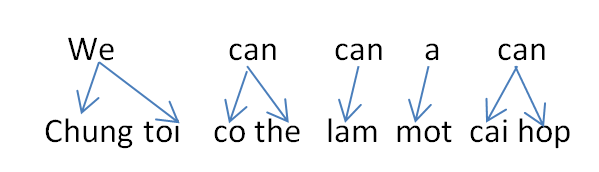
\includegraphics[scale=0.6]{Figures/EN_VI_SAMPLE}
\caption{English - Vietnamese parallel sentence}
\label{fig:EnViparallel}
\end{figure}

\begin{table}
  \centering
    \begin{tabular}{l|c}
    \textbf{Language} & \textbf{Native Speaker(millions)} \\
	\hline
	Bengali & 181 \\
    Javanese & 84.6 \\
    Lahnda & 78.3 \\
    Telugu & 70 \\
    Vietnamese & 69 \\
    Tamil & 65.7 \\
    ... & ...\\
    \end{tabular}%
	 \caption{Major languages with less annotated data 
	 }
  \label{tab:majorLanguageLessData}%
\end{table}%


\section{Universal Tagset}
The universal tagset is the tagset used for our universal tagger. One goal of universal tagger is to motivate the comparison between languages. Thus, universal tagset should be the common denominator of all languages. We adopt the work of \cite{UniversalTagSet} on 12 universal tags which is described in Table \ref{tab:univesalTagset}. We believe that this basic 12 tags are shared among most languages of the world. 
\begin{table}
  \centering
    \begin{tabular}{|c|p{12cm}|}
    \hline
	Tag & Description\\
	\hline \hline
	NOUN & nouns \\
	VERB & verbs\\
	ADJ & adjectives \\
	ADV & adverbs \\
	PRON & pronouns \\
	DET & determiner and articles \\
	ADP & preposition and postpositions\\
	NUM & numerals \\
	CONJ & conjuctions \\
	PRT & particles \\
	. & punctuation marks \\
	X & all other categories such as foreign word, abbreviation etc.\\
	\hline
    \end{tabular}
  \caption{12 tags of the Universal tagset  }    
  \label{tab:univesalTagset}%
\end{table}%
% Benefit of universal tagset 
The universal tagset benefits downstream applications that work across languages such as multilingual taggers, multilingual parsers and so forth. With the consensus tagset, the questions such as ``Tagging language A is harder than language B" would become easier to answer. Moreover, the universal tagger exploits the idea of projecting tag information from a resource-rich language to a resource-poor one. Adopting the universal tagset means that we do not need to care about matching between different tagsets. In addition, we do not have any official tagset for many widely spoken languages such as Telugu or Vietnamese. In this case, a universal tagset would be a good start. 

Nevertheless, we acknowledge that we are loosing information using universal tagset. For example, all \textit{VB, VBD, VBG, VBN, VBP, VBZ} tags from Penn treebank tagset are mapped to \textit{VERB} of Universal tagset. However, this is the trade-off we need to make. % Trade off of content 
\namecite{UniversalTagSet} also provided the mapping from many other tagsets to Universal tagset. Table \ref{tab:tagAccuracySample} lists all the available mapping from each language specific tagset to Universal tagset. In many languages the mapping is clear but in some languages it is not that obvious. \namecite{UniversalTagSet} shows an example of Korean where the adjective is missing. They use stative verb to describe the property of objects, hence, stative verb is mapped to \textit{ADJ} in universal tagset. The other example is the tagset used in French Treebank, there are no \textit{NUM} tags. Numbers are tagged as  adjective or nouns case by case. 
% Provide the mapping 
% Draw back of mapping

% TODO : Write automatic mapping here 
Normally, the mapping is done manually by a linguistic expert. However, \namecite{mapToUniversalTagset} also suggested methods to automatically map from language specific tagsets to the universal tagset. 

%%%%%%%%%%%%%% THIS IS TEMP PART, MERGE TO CH3 when finish 
\section{Methodology}

Here we describe our proposed tagger. The key idea is to maximize the
amount of information gleaned from the source language, while limiting
the amount of noise. Our approach contains 2 main steps (1) Building seed model (2) Apply self-training with revision. We describe the seed model and then explain how it is successively refined through self-training and revision.


\subsection{Seed Model}
\label{seedModel}

The first step is to construct a seed tagger from directly-projected
labels. Given a parallel corpus for a source and target language,
Algorithm~\ref{alg:seedmodel} provides a method for building an
unsupervised tagger for the target language. In typical applications,
the source language would be a resource-rich language having a
tagger, while the target language would be resource-poor, lacking a
tagger and large amounts of manually POS-labelled data.


\begin{algorithm}
\caption{Build seed model}
\label{alg:seedmodel}
\begin{algorithmic} [1]
\STATE Tag source side.
\STATE Word align the corpus with Giza++ and remove the many-to-1 mappings.
\STATE Project tags from source to target using the remaining 1-to-1 alignments.
\STATE Select the top $n$ sentences based on sentence alignment score.
\STATE Estimate emission and transition probabilities. 
\STATE Build seed tagger T. 
\end{algorithmic}
\end{algorithm}

Step 2 aligns words from source to target sentences. Words are aligned if they are translation of each other. There are cases where one word from source sentence is matched with exactly one word in the target sentence (one-to-one mapping) or one word in source sentence is mapped with a phrase in target sentence (many-to-one mapping). We eliminate many-to-one alignments (Step 2). Keeping these alignment would give
more POS-tagged tokens for the target side, but also introduce
noise. For example, suppose English and French were the source and
target language, respectively. In this case alignments such as English
\emph{laws (NNS)} to French \emph{les (DT) lois (NNS)} would be
expected \cite{YarowskyAndNgai} as shown in Figure \ref{fig:sampleEn_Fr}. However, in step 3, where tags are projected from the source to target language, If we just copy tag information from English side \textit{NNS} (common noun) to French side, both ``\textit{les}" and ``\textit{lois}" would be tagged as \textit{NNS}. However, this is incorrect for ``\textit{les}" which must be \textit{DT} (determiner). 

 \begin{figure}
 \centering
 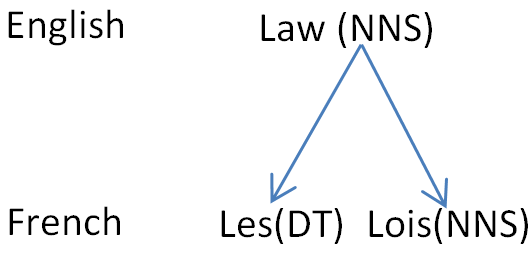
\includegraphics[scale=0.4]{Figures/En_Fr_sample.png}
 \caption{Many-to-one mapping case between English(law) and French(les lois)}
 \label{fig:sampleEn_Fr}
 \end{figure}


We build a French tagger based on English--French parallel data from the Europarl Corpus \cite{europarl}. We want to know the accuracy and coverage of the tags obtained through direct projection. We thus compare these tags again French Melt POS tagger~\cite{DBLP:DenisS09}. This is a supervised French tagger built on French treebank (FTB)~\cite{ftb}. They report the per-token accuracy is as high as 97.80\% and thus, a good approximation for our experiment. Table~\ref{tab:coverageAndAccuracy} confirms
that the one-to-one alignments indeed give higher accuracy but lower
coverage than the many-to-one alignments. One-to-one alignment covers 68\% of the token in French size (that is 32\% is unaligned). However, if we use both one-to-one and many-to-one mapping, we cover 20\% more of the tokens, but the accuracy is dropped by 10\% (absolute). It's worth noting that, accuracy is only calculated from aligned tokens.  Therefore, assuming that we have exactly 1000 tokens, if we used just one-to-one mapping, the number of correctly tagged tokens is $1000 \times 0.68 \times 0.78 = 530$ tokens. The number for additionally use many-to-one mapping is $1000 \times 0.88 \times 0.68 = 598$. That is we have $\frac{598 - 530}{1000} = 6.8$\% more accurately tagged tokens. However, many-to-one introduces more noise (as mentioned in Figure \ref{fig:sampleEn_Fr}), at this stage of the model we hypothesize that high-confidence tags are important, and hence we eliminate the many-to-1 alignments.

\begin{table}
  \small
\tabcolsep 5pt
  \centering
    \begin{tabular}{lcc}
    \hline
	Model & Coverage & Accuracy\\
	\hline 
	Many-to-1 alignments & 88\%& 68\% \\
	1-to-1 alignments    & 68\% & 78\%\\
	1-to-1 alignments: Top 60k sents   & 91\% & 80\%\\
	\hline
    \end{tabular}
  \caption{Token coverage and accuracy of many-to-1 and 1-to-1
    alignments, as well as the top 60k sentences based on alignment
    score for 1-to-1 alignments, using directly-projected labels
    only.}
  \label{tab:coverageAndAccuracy}%
\end{table}%


In Step 4, in an effort to again obtain higher quality target language
tags from direct projection, we eliminate all but the top $n$
sentences based on their alignment scores, as provided by the aligner
via IBM model 3.
%TODO : what is sentence alignment score is ???  How to calculate sentence alignment score ? 
We heuristically set this cutoff to 60k to balance the accuracy and size of the seed model\footnote{We considered values in the range 60--90k, but this choice had little impact on the accuracy of the model. Alternatively, we can set the threshold for sentence alignment score is $10^{-7}$}.
%% PC Is there anything more we can say about choosing the cutoff? Can we
%% briefly summarize the results using other cutoffs?
%% I add the foodnote 
Returning to our preliminary English--French experiments in
Table~\ref{tab:coverageAndAccuracy}, this process gives improvements
in both accuracy and coverage. In the top 60k sentence, we just retain 1-to-1 alignment. The coverage is improved from 68\% to 91\% and the accuracy is also improved from 78\% to 80\%. We also considered using both one-to-one and many-to-one alignments for the top 60k sentences, but in preliminary experiments this did not perform as  well, possibly due to the previously-observed problems with many-to-one alignments. Normally, the higher coverage, the lower accuracy and vice-versa, by simply ranking sentences and choose the first 60k, we have high coverage but in the same time, retain high accuracy. This is a \textit{crucial step} in our proposed methods. 
  
  
%% PC I don't think it's appropriate to be talking about overall accuracy
%% here, because it's confusing given that we're talking about a
%% different type of accuracy in table 1. What would the Coverage and
%% accuracy be for the top 60k sents for the many-to-one alignments?
%% PC I think we could drop this FN to save space.
The step 5 which is for estimating transition and emission probability is based on the following intuition. The number of parameters for the emission probability $p(w|t)$ is $|V| \times |T|$ where $w$ is word, $t$ is tag, $V$ is the vocabulary and $T$ is the tag set. The transition probability $p(t_i|t_{i-1}t_{i-2})$, on the other hand, has only $|T|^3$ parameters
for the trigram model we use. We use the universal tagset, thus, $|T|= 12$ but $|V| \approx 120k$ for French in a preliminary English-French experiment. Because of this huge difference in the number of parameters, in step 5, we employ different strategies to estimate the emission and transition probabilities. The emission probability is estimated from all 60k selected sentences. However, for the transition probability, which has less parameters, we again focus on ``better''
sentences, by estimating this probability from only those sentences
that have 
\begin{enumerate}
\item Token coverage $>90\%$ (based on direct projection of
from the source language)
\item Length $>4$ tokens
\end{enumerate}
These 2 criteria aim to identify longer, mostly-tagged sentences, which we
hypothesize are particularly useful as training data. The underlying reason is that we want to estimate transition probabilities with as small bias as possible. For example, the first token of a sentence is likely to be subject and therefore, \textit{Noun}. If we allow short sentences ($<= 3$ tokens) when calculating trigram transition probability, the model will favor the distribution which start with \textit{Noun}. This is undesirable for our model. In the same idea, a token missing inside a sentence disrupts the normal tag trigram distribution, thus, we reduce this by heuristically choosing only high coverage sentences ($>90$\%) . 


In the case of our preliminary English--French experiments, roughly 62\% of the 60k selected sentences meet these two criteria and are used to estimate the transition probabilities. For unaligned words, we simply assign a random POS and very low probability, which does not substantially affect transition probability estimates. 

In Step 6 we build a tagger by feeding the estimated emission and
transition probabilities into the TNT tagger \cite{TNTTagger}, an
implementation of a trigram HMM tagger.


\subsection{Self training and revision}
\label{selfTrainingAndRevision}
Up to this point we already have a tagger (seed model). In this section, we are going to improve this seed model by applying self-training with special revision. We exploit the large number of target language sentences available that have been
partially tagged through direct projection, in order to build a more
accurate tagger. Back to the preliminary English--French experiments, we just used 60k first sentence for the seed model, however, there are 1.9 millions other sentences. In this part, we are going to exploit the rest of data. 

Algorithm~\ref{alg:selfTraining} describes the
process of self training and revision, and assumes that the parallel
source--target corpus has been word aligned, with many-to-one
alignments removed, and that the sentences are sorted by alignment
score. In contrast to Algorithm~\ref{alg:seedmodel}, all sentences are
used, not just the 60k sentences with the highest alignment scores.

\begin{algorithm}
\caption{Self training and revision}
\label{alg:selfTraining}
\begin{algorithmic} [1]
\STATE Divide target language sentences into blocks of $n$ sentences.
\STATE Tag the first block with the seed tagger.
\STATE Revise the tagged block.
\STATE Train a new tagger on the tagged block.
\STATE Add the previous tagger's lexicon to the new tagger.  
\STATE Use the new tagger to tag the next block.
\STATE Goto 3 and repeat until all blocks are tagged.
\end{algorithmic}
\end{algorithm}

We believe that sentence alignment score might correspond to
the difficulty of tagging. By sorting the sentences by alignment score,
sentences which are more difficult to tag are tagged using a more
mature model.  Following Algorithm~\ref{alg:seedmodel}, we divide
sentences into blocks of 60k. As mentioned before, many-to-one mapping introduce noise, therefore, we just remove it here. 

 \begin{figure}
 \centering
 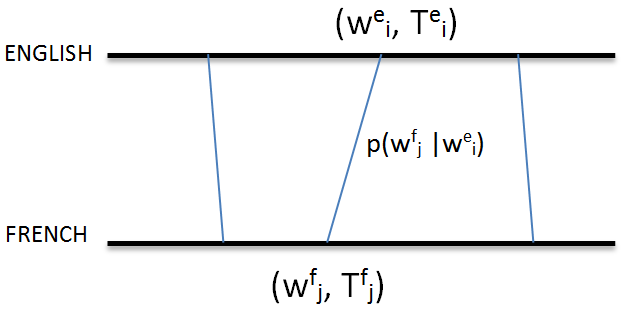
\includegraphics[scale=0.4]{Figures/English_French.png}
 \caption{Alignment between source(English) and target(French) language}
 \label{fig:alignment}
 \end{figure}

In step 3 the tagged block is revised by comparing the tags from the
tagger with those obtained through direct projection. Suppose source
language word $w^e_i$ is aligned with target language word $w^f_j$
with probability $p(w^f_j|w^e_i)$, $T^e_i$ is the tag for $w^e_i$
using the tagger available for the source language, and $T^f_j$ is the
tag for $w^f_j$ using the tagger learned for the target language as shown in Figure \ref{fig:alignment}. If $p(w^f_j|w^e_i) > S$, where $S$ is a threshold which we heuristically set to 0.7, we replace $T^f_j$ by $T^e_i$.  Self-training can suffer from over-fitting, in which errors in the original model are repeated and amplified in the new model \cite{McClosky:2006}.  To avoid this, we remove the tag of any token that the model is uncertain of, i.e.,
if $p(w^f_j|w^e_i) < S$ and $T^f_j \neq T^e_i$ then $T^f_j =
\mathrm{Null}$. So, on the target side, aligned words have a tag from
direct projection or no tag, and unaligned words have a tag assigned
by our model. By keeping the sentences in the order of difficulty to tag, the more we iterate, the more tokens are labeled by maturer model. It also means that, the more we iterate, we trust our model more and the direct projection less as shown in Figure \ref{fig:relianceTagger}. 

 \begin{figure}
 \centering
 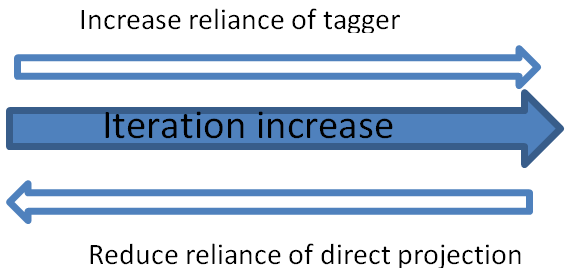
\includegraphics[scale=0.5]{Figures/iterationVsReliance.png}
 \caption{Reliance of tagger and direct projection label}
 \label{fig:relianceTagger}
 \end{figure}


Step 4 estimates the emission and transition probabilities as in
Algorithm~\ref{alg:seedmodel}. In Step 5, emission probabilities for
lexical items presented in the previous model, but missing from the current
model, are added to the current model. Later models therefore take
advantage of information from earlier models, and have wider coverage.

\section{Experiment Detail}
\label{sec:experimentDetail}


In this section, we are going to describe in detail our experiments. In the light of comparing with the state-of-the-art \cite{Das:2011}, we experiment in the way that result would be comparable. 

\subsection{Source data}
Using parallel data from Europarl \cite{europarl} we apply our method
to build taggers for the same eight target languages as
\namecite{Das:2011} --- Danish (da), Dutch (nl), German (de), Greek (el), Italian (it), Portuguese (pt), Spanish (es) and Swedish (sv) --- with English as the source language. \namecite{Das:2011} choose these 8 languages simply because the amount of parallel data for these languages is numerous. Europarl is the corpus collected from European Parliament date back to 1996. At that time, official languages for European Union are only 11 languages. Aside from 8 languages we chose, 3 others are English (en), Finnish (fi) and French (fr). From 2004, European Union expand to 25 members and more languages are added. Thus, due to the long history, the amount of data for these 8 languages we chose are superior compare with most of other languages. 

Our training data (Europarl) is a subset of the training data of
\namecite{Das:2011}, who also used the ODS United Nations dataset
which we were unable to obtain. Less data and as will be shown, the result are comparable, actually make this work stronger than the state-of-the-art. The overview of Europarl for all 8 languages is given in the Table \ref{tab:overviewEuroparl8Lang}. Aside from Greek which has approximately 1.2 million sentences, other language pairs have approximate 1.9 million sentences. 

\begin{table}[htbp]
  \centering

    \begin{tabular}{lrrr}

    \multicolumn{1}{c}{\textbf{Parallel Corpus (L1-L2)}} & \multicolumn{1}{c}{\textbf{Sentences}} & \multicolumn{1}{c}{\textbf{L1 Words}} & \multicolumn{1}{c}{\textbf{English Words}} \\\hline

    Danish-English & 1,968,800 & 44,654,417 & 48,574,988 \\
    Dutch-English & 1,997,775 & 50,602,994 & 49,469,373 \\
    German-English & 1,920,209 & 44,548,491 & 47,818,827 \\
    Greek-English & 1,235,976 & 32,031,068 & 31,929,703 \\
    Italian-English & 1,909,115 & 47,402,927 & 49,666,692 \\
    Portuguese-English & 1,960,407 & 49,147,826 & 49,216,896 \\
    Spanish-English & 1,965,734 & 51,575,748 & 49,093,806 \\
    Swedish-English & 1,862,234 & 41,508,712 & 45,703,795 \\

    \end{tabular}%
    \caption{Overview of Europarl dataset for 8 languages}  
    \label{tab:overviewEuroparl8Lang}%
\end{table}%

\subsection{Word alignment}
After collecting parallel data for each language, we are going to word align the data using the basic open source Giza++ to do the job. However before aligning, we should pre-process the data and pre-compute files needed for alignment. 

\subsubsection{Tokenize the sentence} This step aim at separating each token by a space. It is not as easy as it appear. Model should be able to handle the punctuation well. For example, period ``." which is used as sentence boundary should be separated but not in \textit{``Mr. Paul"} or \textit{``i.e"}. We use an open source \emph{tokenizer.perl} tool from Giza++ package to tokenize both source and target file.

\subsubsection{True casing}
True casing help to choose the most proper casing for each words. For example, the word beginning sentence should be uppercase. However, defining sentence boundary might be tricky. The usual heuristic ``." separate sentences is not always true. For example, ``." in the composition cases such as ``\textit{i.e.}" or ``\textit{Mr.}" does not mark sentence ending.
We also used an open source tool from Giza++ including two steps. (1) Train the model using \emph{train-truecaser.perl}   and (2) true casing using \emph{truecase.perl}. The first steps will output the true casing model which is used in the second step. 

%\begin{verbatim}
%train-truecaser.perl --model ModelFile --corpus input file
%truecase.perl --model ModelFile < input file > output file
%\end{verbatim}

\subsubsection{Cleaning}
Too long sentences are unreliable and not particularly suitable for our task. Therefore, we cut off sentence that longer than 80 words in both side of training data, using \emph{clean-corpus-n.perl} also from Giza++ package.  
%\begin{verbatim}
%clean-corpus-n.perl inPrefix file1 file2 outPrefix 1 80
%\end{verbatim}
%The command will cutoff sentence longer than 80 words from file \texttt{inPrefix.file1 } and \texttt{inPrefix.file2} to form two new files \texttt{outPrefix.file1} and \texttt{outPrefix.file2}. 
The above French-English parallel data from Europarl, approximately 43k (2.2\%) sentences are cutoff. 

\subsubsection{Getting vocabulary and bitext file}
Vocabulary file is needed to run Giza++. It lists the vocabulary and word's frequency in the training data. We must obtain vocabulary file for both source and target language. We use tool $plain2snt.out$ from Giza++ package to build vocabulary for both source and target langauge at once. 
\begin{verbatim}
plain2snt.out source target
\end{verbatim}
The output will be \texttt{source.vcb, target.vcb, source_target.snt, target_source.snt} The first 2 files are vocabulary files for source and target language. The next 2 files are bitext files which represent parallel sentence as  sequence of number. Each number is an id in the vocabulary file. Bitext files are also needed for word alignment. 
%The output will be vocabulary and bitext files for source and target language. Bitext files represent parallel sentence as  sequence of number. Each number is an id in the vocabulary file. Bitext files are also needed for word alignment. 


\subsubsection{Getting word classes}
Word-class files are used just for IBM-model 4/HMM. Syntactic and semantic similar words are grouped into classes. We make use of \emph{mkcls} tool. It's important that word class file name must comply with vocabulary file name. 
\begin{verbatim}
mkcls -psource -Vsource.vcb.classes
mkcls -ptarget -Vtarget.vcb.classes 
\end{verbatim}
%TODO : expand this part if you can 
\subsubsection{Word Alignment}
Everything needed to run word alignment is ready. There are many possible parameters, however, we use the default setting for this experiment. 
\begin{verbatim}
GIZA++ -S source.vcb -T target.vcb -C source_target.snt -o ALIGN
\end{verbatim}
Sometime, co-occurrence file is needed. This file can easily acquire using $snt2cooc.out$ tool. The output would have \texttt{ALIGN} prefix. There are many output files however, we particularly interested in (1) Lexical translation table file i.e. \texttt{ALIGN.t3.final}. (2) Alignment file i.e. \texttt{ALIGN.A3.final}. From these 2 files we will know the alignments and their confidence. Alignment is the most time consuming step in our whole process. To align each language pair in the Europarl corpus, it took us approximately a day on a eight core Intel Xeon 3.16 GHz CPU with 32 Gb Ram. The disadvantage of Giza++ is that, we can not achieve many-to-many mapping. That is, it always aligns from source to target, thus, just produce many-to-one and one-to-one mapping. We can fix this one by running Giza++ from other direction from target to source and merge two results. However, this step will double the running time. We will leave it for future work. 
% Disadvantage OK 

\subsection{Direct tag projection}
We tag the source file (English) with English Stanford POS Tagger \cite{Toutanova:2003}. This available tagger employs Penn treebank tagset which contain of 45 tags. Afterward, we use the mapping from \cite{UniversalTagSet} to map into Universal Tagset (12 tags). Then tags are copied from source side (English) to target side (foreign language) using just one-to-one alignment. 

\subsection{Seed model and final model}
\normalsize
We get sentence score from IBM model 3, that is, \texttt{ALIGN.A3.final}. Sentence score is used to rank sentence.  The following is the sentence pair getting from English-French Europarl parallel data. English sentence \emph{``resumption of the session"} is aligned with French sentence \emph{``reprise de la session"} with sentence alignment score = 0.006578. 


\scriptsize
\begin{lstlisting}
# Sentence pair (1) source length 4 target length 4 alignment score : 0.006578
reprise de la session 
NULL ({ }) resumption ({ 1 }) of ({ 2 }) the ({ 3 }) session ({ 4 }) 
\end{lstlisting}
\normalsize
First 60k sentences are used to build seed model which is described in section (\ref{seedModel}). Then, we use seed model to build final model by applying self-training and revision, section \ref{selfTrainingAndRevision}.

\subsection{Evaluation}
We used the same per-token accuracy evaluation metric as the state-of-the-art~\cite{Das:2011}. Test data for all 8 languages (Danish, Dutch, German, Greek, Italian, Portuguese, Spanish, Swedish) are also the same. These test data which is mainly come from CoNLL-X and CoNLL-07 share tasks. Table \ref{tbl:annotatedData} shows the source and size of test data for each language. We also use the mapping from \cite{UniversalTagSet} to map each language into Universal Tagset. 

\begin{table}
\small
\centering
    \begin{tabular}{lp{3cm}r}
    Language & Source & Number of Words \\
    \hline
    da       & DDT/CoNLL06& 94386           \\
    nl       & Alpino/CoNLL06& 203568          \\
    pt       & Floresta/CoNLL06& 206678          \\
    sv       & Talbanken/CoNLL06& 191467          \\
    el       & GDT/CoNLL07& 65419           \\
    it       & ISST/CoNLL07& 76295           \\
    es       & Cast3LB/CoNLL06& 89334           \\
    de       & Tiger/CoNLL06& 712332          \\
    \end{tabular}
    \caption{Size and source of annotated data}
    \label{tbl:annotatedData}
\end{table}

% List overview of data 
% Just use training data for this task
% Explain mapping process 

\section{Experimental Results}
We experiment as described in previous section \ref{sec:experimentDetail}. 
Using parallel data from Europarl \cite{europarl} we apply our method
to build taggers for the same eight target languages as
\cite{Das:2011} with English as the source language.  Our
training data (Europarl) is a subset of the training data of
\namecite{Das:2011}. The evaluation metric and test data
are the same as that used by \citeauthor{Das:2011}. Our results are
comparable to theirs, although our system is penalized by having less
training data. 

\begin{table}
\small
\tabcolsep 5pt
\begin{center}
\begin{tabular}{lcccccccccc}
        \hline
        ~                      & da & nl & de & el & it & pt & es & sv & & Avg. \\ \hline
        Seed model             & 83.7   & 81.1  & 83.6   & 77.8 & 78.6    & 84.9       & 81.4       & 78.9    & & 81.3   \\ 
        Self training + revision & \textbf{85.6}  & \textbf{84.0}    & \textbf{85.4}   & 80.4  & 81.4   & 86.3       &   83.3     & \textbf{81.0}      & & 83.4   \\ 
        \cite{Das:2011}          & 83.2   & 79.5  & 82.8   & \textbf{82.5}  & \textbf{86.8}    & \textbf{87.9}       & \textbf{84.2}    & 80.5    & & \textbf{83.4}   \\ 
\hline
Prop. of unknown words  & 10.9   & 10.7 & 10.6      & 6.0     & 12.8    & 9.6       & 8.0        & 7.3    & & 9.5   \\
        %% \hline
\end{tabular}
\caption{Token-level POS tagging accuracy for our seed model, self
  training and revision, and the method of \protect\cite{Das:2011}. The best results on each language, and on average, are shown in bold. }
\label{tab:taggingAcc}
\end{center}
\end{table}


Table~\ref{tab:taggingAcc} shows results for our seed model, self
training and revision, and the results reported by
\citeauthor{Das:2011}. Self training and revision improves the
accuracy for every language over the seed model, and gives an average
improvement of roughly two percentage points. The average accuracy of
self training and revision is on par with that reported by
\citeauthor{Das:2011}. On individual languages, self training and
revision and the method of \citeauthor{Das:2011} are split --- each
performs better on half of the cases. Interestingly, our method
achieves higher accuracies on Germanic languages --- the family of our
source language, English --- while \citeauthor{Das:2011} perform
better on Romance languages. This might be because our model relies on
alignments, which might be more accurate for more-related languages,
whereas \citeauthor{Das:2011} additionally rely on label propagation.

The last row of Table~\ref{tab:taggingAcc} shows the percentage of
unknown words for each language on the test data. On average,
approximately 10\% of the test data tokens are unknown. One way to
improve the performance of our tagger might be to reduce the
proportion of unknown words by using a larger training corpus, as
\citeauthor{Das:2011} did. We should also consider corpus that cover wider topics. Language used in Europarl is formal and domain specific such as news, politic, economic etc. However, test data covers many more subjects such as fiction, sport etc. That might be the reason why despite Europarl is a very huge corpus, unknown word (OOV) rate is still high. 


 \begin{figure}
 \centering
 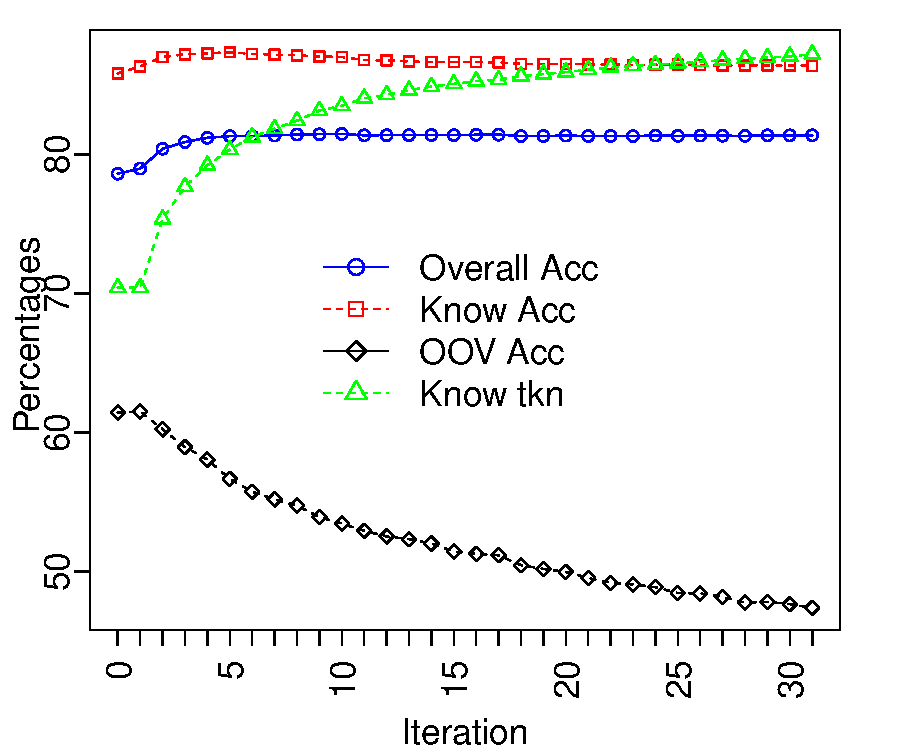
\includegraphics[scale=0.7]{Figures/itAcc}
 \caption{Overall accuracy, accuracy on known tokens, accuracy on
   unknown tokens, and proportion of known tokens for Italian.}
 \label{fig:italian}
 \end{figure}

Compared to \namecite{Das:2011}, our model performs poorest on
Italian, in terms of percentage point difference in accuracy.
Figure~\ref{fig:italian} shows accuracy,
accuracy on known words, accuracy on unknown words, and proportion of
known tokens for each iteration of our model for Italian. Iteration 0
is the seed model, and iteration 31 is the final model. Our model
performs poorly on unknown words as indicated by the low accuracy on
unknown words. The ``overall accuracy" line is always between ``known accuracy" and ``unknown accuracy" line weighted by ``proportion of known tokens" line. Thus, despite unknown words' accuracy drops drastically from 62\% to 47\%, an overall accuracy still (slightly) increases thank to increment on known accuracy words and proportion of known tokens. 

The poor performance on unknown words is expected because we do not use any language-specific rules to handle this case. Moreover, for the final model, approximately 13\% of the test data tokens are unknown.  This is the highest rate compare to other languages as in Table \ref{tab:taggingAcc}. This also partially explain why performance is poor on Italian. 

 \begin{figure}
 \centering
 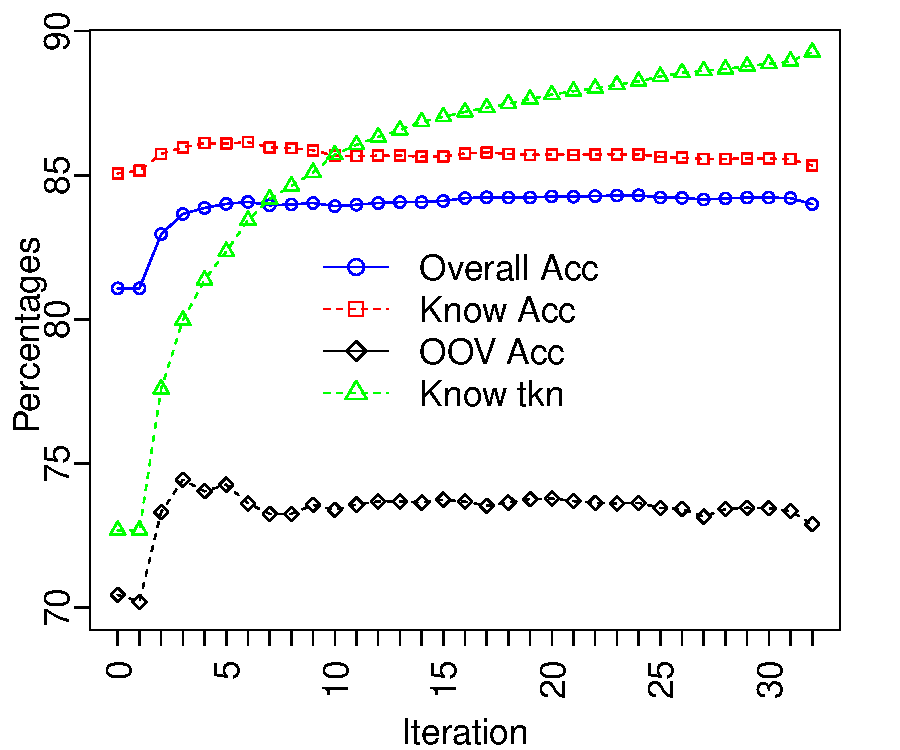
\includegraphics[scale=0.7]{Figures/nlAcc}
 \caption{Overall accuracy, accuracy on known tokens, accuracy on
   unknown tokens, and proportion of known tokens for Dutch.}
 \label{fig:dutch}
 \end{figure}

We examine the impact of self-training and revision over training
iterations. We find that for all languages, accuracy rises quickly in
the first 5--6 iterations, and then subsequently improves only
slightly. We exemplify this in Figure~\ref{fig:dutch} for Dutch, findings are similar for other languages. Although accuracy does not increase much in later iterations, they may still have some benefit as the vocabulary size continues to grow.

\section{Summary of Contributions}

We have proposed a method for unsupervised POS tagging (Universal tagger) that performs on par with the current state-of-the-art \cite{Das:2011}, but is substantially less-sophisticated (specifically not requiring convex 
optimization or a feature-based HMM). The complexity for fully optimizing a convex function is $O(n^3)$ where $n$ is size of data. This complexity is impractical because $n$ is very big ($n \approx $ 2 millions). \namecite{Das:2011} avoid this by just optimize for 10 iterations, instead of looping until converge. The complexity for each iteration is $O(n^2)$. So the overall complexity is $O(n^2)$. The complexity of our algorithm, on the other hand, is just $O(nlogn)$. This complexity is derived from sentence score sorting operation. The huge difference in complexity resulting in substantial running speed variance. We re-implemented label propagation from \cite{Das:2011}. It took over a day to complete this step on an eight core Intel Xeon 3.16 GHz CPU with 32 Gb Ram, but only 15 minutes for our model.  Moreover, unlike \namecite{Das:2011} who can not publish their code due to company license restriction, we made our code available for download\footnote{https://code.google.com/p/universal-tagger/} which hopefully will aid the development of multilingual natural language processing (NLP).

In future work we intend to consider using a larger training corpus to reduce the proportion of unknown tokens and improve accuracy. We can align source and target language in both directions, i.e.\ from source to target and from target to source language. Merging two alignment might yield a better one-to-one mapping set.

Given the improvements of our model over that of \citeauthor{Das:2011} on languages from the same family as source language, and the observation of
\namecite{SnyderMultilingualPOS} that a better tagger can be learned from
a more-closely related language, we also plan to consider strategies
for selecting more appropriate source language for a given target
language. 

Using our final model with unsupervised HMM inference methods might improve the final performance too, i.e.\ use our final model as the initial state for HMM, then experiment with different inference algorithms such as Expectation Maximization (EM), Variational Bayers (VB) or Gibbs sampling (GS). We in fact have tried EM, but it did not help. The overall performance dropped slightly. This might be because self-training with revision already found the local maximal point. However, VB or GS might help. \namecite{Gao:2008} compare EM, VB and GS for unsupervised English POS tagging. In many cases, GS outperformed other methods, thus we would like to try GS first for our model. 



% Chapter 4: Source language(s) selection
%%%% NEXT CHAPTER #################################################
%##################################################################

\chapter{Source Language Selection}
\label{chap:sourceLanguageSelection}

Bilingual corpora offer a promising bridge between resource-rich and resource-poor languages, enabling the development of multilingual NLP technologies for a far wider range of languages.  In the previous chapter, we used bilingual corpora to build a tagger for the target language. Its performance is on par with the state-of-the-art \cite{Das:2011}. In this chapter we would like to further improve our tagger by investigating source language factors. English is often used as a source language, but it is not the only available
resource-rich language, and another choice may have a dramatic effect
on performance. Where multiple source languages are available, what should we do? How can we combine them? The relationship of source language selection and the universal tagger will be thoroughly considered in this chapter. 

\section{Introduction}

Parallel texts are becoming increasingly available through
sources such as multilingual websites, multilingual documents and large archives of translation memory from books, news. Not only the size but also the number of languages covered by parallel data is increasing. The era of English dominating one side of parallel texts is shifting to a far wider range of languages. Parallel data can be exploited to bridge languages, and in particular, transfer annotated information from a highly-resourced \emph{source} language to a lesser-resourced
\emph{target} language, to build unsupervised POS taggers as demonstrated in Chapter  \ref{chap:uniTagger}. 

One issue in building such a tagger is choosing the source
language. English is commonly used, because parallel data which has
English on one side is often most readily available. However, the
appropriate source language might depend on the target language. 
% Motivation 
Chapter \ref{chap:uniTagger} shows that taggers for languages which are in the same language family tree (Germanic) with source language (English) perform better than the state-of-the-art \cite{Das:2011}. \namecite{SnyderMultilingualPOS} suggested that performance of Slovene tagger improves 7.69\% (absolute) when paired with Serbian, a very closely related language, but only 1.3\% when paired with English. \namecite{reddy2011crosspos} and \namecite{Hana04} show that for closely related languages, the transition probabilities for an HMM tagger can be
used interchangeably.  This experience demonstrates that the choice of
source language might have a drastic effect on target language tagger performance. Moreover, if parallel data for a target language with more than one source language is available, it might be possible to exploit this additional information; however, this issue has not been explored to date. Thus, in this chapter we investigate the problem of making a good choice of source language(s).

% Added overview of paper

In this chapter we are going to build unsupervised POS taggers for $m$ language
pairs using the tagger from chapter \ref{chap:uniTagger}. We identify features --- derived from both monolingual and parallel corpora --- that we could use to predict the best source language to build a tagger for a given target language. We show that choosing an appropriate source language can improve the accuracy of our
state-of-the-art unsupervised POS tagging methodology, compared to
using a single fixed source language. This prediction can be done
based on features of the source and target language derived from
monolingual corpora, although further improvements can be obtained
using the features based on parallel corpora. We then show that even
better accurate prediction can be obtained by incorporating information from
multiple source languages. 

Formally speaking, assuming that we need to build tagger for target language $t$, we have all possible source languages  $s_1,s_2...s_n$. In this chapter, we are going to answer two questions: (1)~what is the best source language $s_i$? (2)~Can we do better by combining multiple source languages? To answer these two questions, we experiment as follows:

%% The first question when building this kind of tagger is choosing the
%% source language. People normally use English as parallel data which
%% has English in one side is easier to acquire. However, is English a
%% good choice? What we should do if we have more than one possible
%% source language. Formally, assuming that we need to build tagger for
%% target language $y$, we have all possible source language
%% $x_1,x_2...x_n$. In this paper, we are trying to answer two questions
%% such that, (1) \textit{``what is the best source language $x_i$?"} (2)
%% \textit{``What if we combine multiple source languages?"}. 

 \begin{enumerate}
 \itemsep0em
 \item Pick $n$ languages  (Section \ref{sec:collectParaData})
 \item Collect $ n \times (n-1)$ parallel data sets (Section \ref{sec:collectParaData})
 \item Define features (Section \ref{featuresSec})
 \item Using parallel data from each language pair, build the tagger (Section \ref{sec:buildTagger})
 \item Build a source language predicting model based on the features (Section \ref{sec:sourceLanguagePrediction})
 \item Combine multiple source languages (Section \ref{sec:multipleSourceLanguages})
 \end{enumerate}

%% Kind of motivation here, I don't think we should move to related work part. 

\section{Collect parallel data}
\label{sec:collectParaData}
We would like to conduct experiments on a resource-poor target language, however, it would be much harder to evaluate. We instead experiment with the same $n = 9$ languages (English, Danish, Dutch, Portuguese, Swedish, Greek, Italian, German, Spanish).  We use the JRC-Acquis corpus which provides parallel data for every pair of 22 European languages~\cite{SteinbergerAcquis}. We thus, extract a subset of 72 language pairs. It's worth noting that we consider ($x-y$) and ($y-x$) to be two different language pairs. 

JRC-Acquis contains of EU legislation, rights, agreements, declarations etc that must be translated to all participating EU countries (currently 22). Thus, theoretically, each document would have a translation into 21 other languages. However, many documents for some languages are unavailable. Only documents that have translation into at least 10 other languages are included in the JRC-Acquis corpus. 

To the best of our knowledge, JRC-Acquis is the biggest corpus providing parallel data for all of the language pairs we consider. Table~\ref{tab:acquis} shows some monolingual statistics about each language. Table \ref{tab:jrcAcquisSizeEachPair} shows the size of parallel data (number of sentences) for each language pair. It is clear that, parallel data in JRC-Acquis is balanced, that is, the size of each language pair is approximately the same. 
%Moreover, the number of texts for each language are also similar to each other (Table \ref{tab:acquis}). We can induce that, majority of text are shared across languages.  
%% Some statistic about data 
\begin{table}
\small
\centering
    \begin{tabular}{ccc}
    Language & No.\ of Texts & No.\ of Words ($\times 10^6$) \\
    \hline
    en       & 23545       & 55.5     \\
    da       & 23624       & 50.9     \\
    nl       & 23564       & 56.8     \\
    pt       & 23505       & 59.6     \\
    sv       & 20243       & 47.0     \\
    el       & 23184       & 55.9     \\
    it       & 23472       & 57.2     \\
    es       & 23573       & 62.1     \\
    de       & 23541       & 50.9     \\
    \end{tabular}
    \caption{The number of texts and words for each language considered in the JRC-Acquis corpus.}
    \label{tab:acquis}
\end{table}


\begin{table}[htbp]
  \centering

    \begin{tabular}{r|rrrrrrrrr|r}
          & en    & da    & nl    & pt    & sv    & el    & it    & es    & de    & Avg \\\hline
    en    & -     & 1.00  & 1.13  & 1.12  & 1.06  & 0.79  & 1.12  & 1.12  & 1.14  & 1.06 \\
    da    & 1.00  & -     & 1.16  & 1.14  & 1.10  & 0.83  & 1.14  & 1.14  & 1.16  & 1.10 \\
    nl    & 1.13  & 1.16  & -     & 1.13  & 1.07  & 0.85  & 1.14  & 1.13  & 1.14  & 1.09 \\
    pt    & 1.12  & 1.14  & 1.13  & -     & 1.05  & 0.84  & 1.13  & 1.13  & 1.12  & 1.08 \\
    sv    & 1.06  & 1.10  & 1.07  & 1.05  & -     & 0.77  & 1.06  & 1.05  & 1.08  & 1.03 \\
    el    & 0.79  & 0.83  & 0.85  & 0.84  & 0.77  & -     & 0.84  & 0.86  & 0.89  & 0.83 \\
    it    & 1.12  & 1.14  & 1.14  & 1.13  & 1.06  & 0.84  & -     & 1.13  & 1.13  & 1.09 \\
    es    & 1.12  & 1.14  & 1.13  & 1.13  & 1.05  & 0.86  & 1.13  & -     & 1.12  & 1.08 \\
    de    & 1.14  & 1.16  & 1.14  & 1.12  & 1.08  & 0.89  & 1.13  & 1.12  & -     & 1.10 \\
    \end{tabular}%
  \caption{JRC-Acquis corpus size ($\times 10^6$) for every language pair.}
  \label{tab:jrcAcquisSizeEachPair}%
\end{table}%

Intuitively, there is the question why we do not use the same Europarl parallel corpus as in chapter \ref{chap:uniTagger}. Europarl provides parallel data which has English on one side. We can always create other language pairs by using English as a pivot language. However, apart from the language pairs that involve English, all the other language pairs have more substantial coverage in JRC-Acquis. This means that Europarl is English-oriented and not particularly suitable for our experiment. Table \ref{tab:europarlCorpusSize} shows the size of each language pair (number of sentences) obtained from Europarl. The average data size for parallel data having English as the source language is double or triple compared to the other languages. 

\begin{table}[htbp]
  \centering

    \begin{tabular}{r|rrrrrrrrr|r}
          & en    & da    & nl    & pt    & sv    & el    & it    & es    & de    & Avg \\\hline

    en    & -     & 1.97  & 2.00  & 1.96  & 1.86  & 1.24  & 1.91  & 1.97  & 1.92  & 1.85 \\
    da    & 1.97  & -     & 0.34  & 0.38  & 0.43  & 0.98  & 0.54  & 0.35  & 0.40  & 0.68 \\
    nl    & 2.00  & 0.34  & -     & 0.39  & 0.44  & 1.05  & 0.53  & 0.39  & 0.42  & 0.69 \\
    pt    & 1.96  & 0.38  & 0.39  & -     & 0.45  & 1.03  & 0.54  & 0.38  & 0.44  & 0.70 \\
    sv    & 1.86  & 0.43  & 0.44  & 0.45  & -     & 0.97  & 0.63  & 0.45  & 0.48  & 0.71 \\
    el    & 1.24  & 0.98  & 1.05  & 1.03  & 0.97  & -     & 1.11  & 1.01  & 1.06  & 1.06 \\
    it    & 1.91  & 0.54  & 0.53  & 0.54  & 0.63  & 1.11  & -     & 0.54  & 0.59  & 0.80 \\
    es    & 1.97  & 0.35  & 0.39  & 0.38  & 0.45  & 1.01  & 0.54  & -     & 0.43  & 0.69 \\
    de    & 1.92  & 0.40  & 0.42  & 0.44  & 0.48  & 1.06  & 0.59  & 0.43  & -     & 0.72 \\

    \end{tabular}%
  \caption{Europarl corpus size ($\times 10^6$) for every language pair. Where suitable bilingual data is not available, English is used as a pivot language to derived the other language pair.}
  \label{tab:europarlCorpusSize}%
\end{table}%


\section{Features}
\label{featuresSec}
In this section, we consider factors that influence the choice of source language. We divide the features into two categories: \textit{monolingual features} which exploit only monolingual data, and \textit{bilingual features} which exploit parallel data. 

\subsection{Monolingual features}
\begin{table}
\small
\centering
    \begin{tabular}{cccc}
   \multirow{2}{*}{Language} &  \multicolumn{2}{c}{Corpus Size}  & \multirow{2}{*}{Voc.\ Size} \\\cline{2-3}
         &  Acquis & Europarl &  \\\hline
    en              & - &  -       & 14810           \\
    da              & 1000785 &  1968800       & 29867           \\
    nl              & 1132352 &  1997775          & 21316           \\
    pt              & 1121460 &  1960407           & 19333           \\
    sv              & 1061156 &  1862234          & 29403           \\
    el              & 792732  &  1235976          & 34992           \\
    it              & 1122016 &  1909115          & 19310           \\
    es              & 1117322 &  1965734         & 18496           \\
    de              & 1136452 &  1920209          & 29860           \\
    \end{tabular}
    \caption{Corpus size (number of tokens) and vocabulary size, for
      each language, with English as the source language.}
    \label{tbl:corpsizeVocSize}
\end{table}

%% \subsubsection{Morphological complexity}

\subsubsection{Morphological complexity} 

Morphologically rich languages introduce complexity when aligning parallel data because there is much greater ambiguity in alignment. Given the reliance of our approach on high quality alignments, morphological complexity is an important factor to consider. We can estimate morphological complexity by counting the number of unique tokens, i.e.\ the vocabulary size. In table~\ref{tbl:corpsizeVocSize}, Voc.\ Size column displays vocabulary estimates for each language, assuming a corpus of a million words. This estimate uses the source side of the Acquis Corpus, although any monolingual corpus would suffice.  

%% PC: Need to clarify why no numbers are given for English in Table 2.
%% There is number for english for Voc.Size in table 2, I just add the column specific for this one. 


\subsubsection{Language relatedness}
%% \label{sec:langRelatedness}

Our nine languages belong to three
language families: Germanic (English, Danish, Dutch, Swedish, German);
Romance (Portuguese, Italian, Spanish), and Baltic
(Greek). Previously in chapter \ref{chap:uniTagger}, our Universal Tagger performed better than the state-of-the-art on four languages which are in the same language family (Germanic) as the source language (English). Thus, language relatedness is an important factor to consider.

We quantify language relatedness using lexicostatistics on the Swadesh 200 word list \cite{Meyer92}. Table \ref{tab:swadeshList} shows examples of some meanings in English. This list was chosen by linguist Morris Swadesh by carefully taking into consideration cultural independence and attestation in many languages. The Swadesh word list is sometimes called a ``universal" vocabulary because these meanings appear in the largest number of languages. The Swadesh list is important in lexico-statistics for studying language relatedness using the method of glottochronology. 

\begin{table}[htbp]
  \centering

    \begin{tabular}{rrr}
    I     & louse & tooth \\
    and   & blood & know \\
    all  & bone  & die \\
    who   & egg   & give \\
    father  & animal  & sun \\
    one   & tail  & moon \\
    two   & ear   & water \\
    fish  & eye   & salt \\
    dog   & nose  & stone \\
    \end{tabular}%
  \caption{Some meanings from the Swadesh word list}
  \label{tab:swadeshList}%
\end{table}%

Lexicostatistics involves the judgment of linguist about whether a given pair of words are cognates or not. Two words are cognate if they evolved from the same ancestor. For example ``\textit{night}" (English), ``\textit{nuit}" (French) and \textit{``Nacht"} (German) are cognate because they all derived from Proto-Indo-European word ``\textit{nokwts}"\footnote{http://en.wikipedia.org/wiki/Cognates}. 

The relatedness of two languages is just the percentage of shared cognates in the word list. For example, Table \ref{tab:langRelatednessMeasure} measures the relatedness  between German and Spanish. Assume that for all 200 meanings, there are 90 ``yes" in the \emph{Cognate} column, the language relatedness of German and Spanish would be $\frac{90}{200} = 0.45 $. Note that this measurement is symmetric. Two languages are considered close to each other if this value is high (close to 1). The postulation of language families is also partially based on this measurement. Languages that are close to each other are grouped into the same family. 

\begin{table}[htbp]
  \centering

    \begin{tabular}{llccc}
    No. & Meaning & German & Spanish & Cognate \\\hline
    1 & all   & alle  & todo  & no \\
    2 & and   & und   & y     & no \\
    3 & father & Vater & padre & yes \\
    4 & animal & Tier  & animal & no \\
    .. & .. & .. & .. & .. \\
    200 & I     & Ich   & yo    & yes \\

    \end{tabular}%
  \caption{Language relatedness measure between German and Spanish}
  \label{tab:langRelatednessMeasure}%
\end{table}%
\namecite{Meyer92} provides a table showing the language relatedness measurements for all 84 Indo-European languages. We thus extract a subset of 36 language pairs from this list. The extracted data is shown in Table \ref{tab:langRelatedNess9Lang}\footnote{for some language pairs, there are some meanings that do not present in these languages, thus, the final number is only calculated on a subset of 200 meanings}.

\begin{table}[htbp]
  \centering
    \begin{tabular}{r|rrrrrrrrr}
          & en    & da    & nl    & de    & el    & it    & pt    & es    & sv \\\hline
    en    & -     & 0.593 & 0.593 & 0.578 & 0.162 & 0.247 & 0.24  & 0.24  & 0.589 \\
    da    & 0.593 & -     & 0.663 & 0.707 & 0.183 & 0.263 & 0.25  & 0.25  & 0.874 \\
    nl    & 0.593 & 0.663 & -     & 0.838 & 0.188 & 0.26  & 0.253 & 0.258 & 0.692 \\
    de    & 0.578 & 0.707 & 0.838 & -     & 0.188 & 0.265 & 0.247 & 0.253 & 0.695 \\
    el    & 0.162 & 0.183 & 0.188 & 0.188 & -     & 0.178 & 0.167 & 0.167 & 0.184 \\
    it    & 0.247 & 0.263 & 0.26  & 0.265 & 0.178 & -     & 0.773 & 0.788 & 0.259 \\
    pt    & 0.24  & 0.25  & 0.253 & 0.247 & 0.167 & 0.773 & -     & 0.874 & 0.258 \\
    es    & 0.24  & 0.25  & 0.258 & 0.253 & 0.167 & 0.788 & 0.874 & -     & 0.253 \\
    sv    & 0.589 & 0.874 & 0.692 & 0.695 & 0.184 & 0.259 & 0.258 & 0.253 & - \\

    \end{tabular}%
  \caption{Language relatedness measure for 9 languages}
  \label{tab:langRelatedNess9Lang}%
\end{table}%
%% We use this feature as a baseline for the source language predicting model. 

\subsection{Bilingual features}

% introduce this section?

% do we need separate subsections here? later xrefs could mention these features by name, without needing to cite section numbers.
\paragraph{Corpus size}
The most obvious feature is corpus size. The more data we have, the better. We count the number of parallel sentences in the corpus.  Table~\ref{tbl:corpsizeVocSize} shows the corpus size for each language pair with English as the source side. 

\paragraph{One-to-One alignment proportion}
%% \label{sec:oneToone}
We believe that one-to-one mapping is more meaningful for the task than many-to-one mapping. The intuition is that if there is only one possible way to copy a tag from the source language to the target language, we can be more confident about the mapping. The proportion of one-to-one mappings is calculated using a fixed number of parallel sentences (800k sentences) for all languages.  

\paragraph{Sentence alignment score}
%% \label{sec:sentScore}
Sentence alignment scores are provided by the aligner from IBM Model 3.  We used these scores to rank sentences in building a seed model as in chapter \ref{chap:uniTagger}. This score has proven to be effective in choosing high quality sentences. Higher alignment scores might therefore correspond to a more accurate tagger. We use the average sentence alignment score for each language pair as a feature.


%% We can easily extract sentence alignment scores as provided by the aligner for IBM Model 3.  \cite{Duong:2013} used sentence alignment scores to rank sentences in building their tagger, showing that this is effective in choosing high quality sentences. Higher alignment scores might therefore correspond to a more accurate tagger. Thus, we incorporate the average sentence alignment score for each language pair into feature list.  

%% PC: What is this feature specifically? Average sentence alignment score?
%% That's right, the average sentence alignment score (Added)

\paragraph{Lexical translation entropy}
%% \label{sec:transEntropy}

We adopt the idea of translation model entropy from \cite{462MTSystem}. However, instead of scanning all possible sentence segmentations and calculating the phrase-based entropy, we employ a simpler method based on the lexical translation table. That is, the entropy for each lexical entry is calculated as $$H(s) = -\sum_{t\in T} p(t|s)\times log_2 p(t|s)$$ where $T$ is a possible translation of word $s$. For each language, we pick a fixed amount of text (1 million words) and calculate the average entropy for all words.  

%% Although these three alignment features are somewhat correlated, we
%% treat them as distinct features.
% SB: it would be nice to say why this is ok - how important is the independence assumption?
% are they only slightly dependent?
%% PC: Cut because we didn't have a response to Steven's comment, and by
%% drawing attention to it without motivation I thought we weakened the
%% paper.


\section{Build taggers}
\label{sec:buildTagger}
In this section we construct 72 taggers, using parallel data for 72
language pairs, and then evaluate the performance of each pair. We
use the Universal tagger from chapter \ref{chap:uniTagger}. Constructing a tagger for each language pair involves word alignment which is computationally expensive. Thus, we distribute the computation to four servers. Each server run multiple threads but it still took over 3 days for the whole process. 

Our Universal tagger employs the consensus 12 Universal Tagset \cite{UniversalTagSet},\footnote{NOUN, VERB, ADJ, ADV, PRON (pronouns), DET (determiners and articles), ADP (prepositions and postpositions), NUM (numerals), CONJ (conjunctions), PRT (particles), ``.'' (punctuation), and X (all  other categories, e.g., foreign words, abbreviations). } to avoid the problem of transliterating between different tagsets for different languages. Using this consensus tagset is crucial for enabling comparison across languages. 
The input for the Universal Tagger is a tagger for the source language $Tagger(s)$, along with parallel data $(s-t)$. The source language $s$ is tagged using $Tagger(s)$, and then the tagged labels are projected to the target language side $t$. We rank and build a seed model $T_0$ on just the high scoring sentences. By applying self-training with revision, a series of new models is constructed $T_1,T_2,\ldots,T_m$. The output tagger for the target language is the last model $Tagger(t) = T_m$.

$Tagger(s)$ is trained from manually annotated data $Data(s)$ which is mainly derived from the CoNLL 06 and CoNLL 07 Shared Tasks. (Table~\ref{tbl:annotatedDataNew} shows the source and size of annotated data for each language.) It is worth noticing that we only train on labeled data for the source language not for the target language. This means that training and testing data are always different for all language pairs. The annotated data was also used in the previous chapter \ref{chap:uniTagger} for evaluating the target tagger. We believe that the size of manually tagged corpus for each language is sufficient for building a reliable supervised POS tagger. Using the matching provided by \namecite{UniversalTagSet}, we map the individual tagsets to the Universal Tagset. We train a supervised POS tagger $Tagger(s)$ on the annotated data using the TNT tagger \cite{TNTTagger}. This data is also used for evaluating the target language tagger $Tagger(t)$. 
\begin{table}
\small
\centering
    \begin{tabular}{lp{3cm}r}
    Language & Source & Number of Words \\
    \hline
    en       & WSJ/PennTB & 1,289k         \\
    da       & DDT/CoNLL06& 94k           \\
    nl       & Alpino/CoNLL06& 203k          \\
    pt       & Floresta/CoNLL06& 206k          \\
    sv       & Talbanken/CoNLL06& 191k          \\
    el       & GDT/CoNLL07& 65k           \\
    it       & ISST/CoNLL07& 76k           \\
    es       & Cast3LB/CoNLL06& 89k           \\
    de       & Tiger/CoNLL06& 712k          \\
    \end{tabular}
    \caption{Size and source of annotated data}
    \label{tbl:annotatedDataNew}
\end{table}


\begin{table}
\centering
%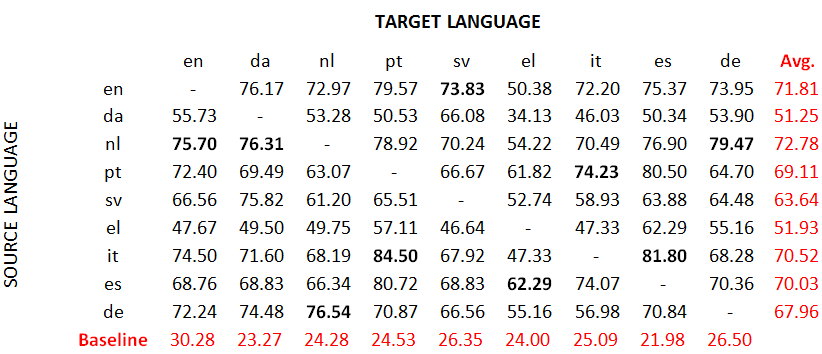
\includegraphics[scale=0.7]{Figures/TaggerPerformance}
\setlength{\tabcolsep}{3pt}
    \begin{tabular}{rccccccccccc}

          & \multicolumn{11}{c}{TARGET LANGUAGE} \\
          &       & en    & da    & nl    & pt    & sv    & el    & it    & es    & de    & \textbf{Avg.} \\
    \multicolumn{1}{c}{\multirow{10}[0]{*}{
	\begin{sideways}  
    SOURCE LANGUAGE
    \end{sideways}
}} & en    & -     & 76.17 & 72.97 & 79.57 & \textbf{73.83} & 50.38 & 72.20 & 75.37 & 73.95 & 71.81 \\
    \multicolumn{1}{c}{} & da    & 55.73 & -     & 53.28 & 50.53 & 66.08 & 34.13 & 46.03 & 50.34 & 53.90 & 51.25 \\
    \multicolumn{1}{c}{} & nl    & \textbf{75.70} & \textbf{76.31} & -     & 78.92 & 70.24 & 54.22 & 70.49 & 76.90 & \textbf{79.47} & 72.78 \\
    \multicolumn{1}{c}{} & pt    & 72.40 & 69.49 & 63.07 & -     & 66.67 & 61.82 & \textbf{74.23} & 80.50 & 64.70 & 69.11 \\
    \multicolumn{1}{c}{} & sv    & 66.56 & 75.82 & 61.20 & 65.51 & -     & 52.74 & 58.93 & 63.88 & 64.48 & 63.64 \\
    \multicolumn{1}{c}{} & el    & 47.67 & 49.50 & 49.75 & 57.11 & 46.64 & -     & 47.33 & 62.29 & 55.16 & 51.93 \\
    \multicolumn{1}{c}{} & it    & 74.50 & 71.60 & 68.19 & \textbf{84.50} & 67.92 & 47.33 & -     & \textbf{81.80} & 68.28 & 70.52 \\
    \multicolumn{1}{c}{} & es    & 68.76 & 68.83 & 66.34 & 80.72 & 68.83 & \textbf{62.29} & 74.07 & -     & 70.36 & 70.03 \\
    \multicolumn{1}{c}{} & de    & 72.24 & 74.48 & \textbf{76.54} & 70.87 & 66.56 & 55.16 & 56.98 & 70.84 & -     & 67.96 \\
    \multicolumn{1}{c}{} & \textbf{Baseline} & 30.28 & 23.27 & 24.28 & 24.53 & 26.35 & 24.00 & 25.09 & 21.98 & 26.50 &  \\
    \end{tabular}%


\caption{Tagger accuracy for each source--target language pair. The best tagger for each target language is shown in bold.}
\label{fig:taggerPerformance}
\end{table}

We evaluate each $Tagger(t)$ using $Data(t)$, and report the results
shown in Table~\ref{fig:taggerPerformance}. The average tagger
performance for each source language is also given. It turns out that
choosing Dutch (avg =72.78\%) as the source language rather than
English (avg=71.81\%) gives the best overall performance. The tagger
performance of each target language is much better than the baseline
that always picks the most frequent tag for each word.\footnote{For most of languages, the baseline is assigning ``Noun" for all words.} 

The Greek tagger performs poorly. From Table \ref{tbl:corpsizeVocSize}, Greek is the most morphologicaly complex language in this set, and has the smallest corpus size, two factors which partially explain why tagger performance for Greek is low regardless of whether Greek occupies the source or target language role. 

From Table~\ref{fig:taggerPerformance}, it seems that taggers perform better if the source and target language are in the same language family. For example, the top four source languages for Danish are English, Dutch, Swedish and German, and the top two source languages for Portuguese are Italian and Spanish. This confirms the intuition in adding language relatedness features in section \ref{featuresSec}. 

In chapter \ref{chap:uniTagger}, we also used English as the source language to build taggers for the same eight other languages. The only difference between these two experiments is that in chapter \ref{chap:uniTagger} experiment, we used Europarl \cite{europarl} data instead of JRC-Acquis. Table~\ref{tbl:acc2Models} compares the performance of each target language using English as the source language, for the two datasets. As mentioned before, Europarl is English oriented and not relevant for our experiment. Table~\ref{tbl:corpsizeVocSize} also compares the size of parallel
data having English as the source language, for both corpora. Given
that Europarl is much larger, higher performance is expected. However,
Table~\ref{tbl:acc2Models} shows a strong correlation between the two
experiments (Pearson's $r$ = 0.7).\footnote{The common rule of thumb interpretation for Pearson-correlation is as follows: $|r| > 0.7$ : very strong relationship, $> 0.4$ : strong relationship, $> 0.3$ : moderate relationship, $> 0.2$ : weak relationship, $>0.01$: no or negligible relationship. Negative r means a negative relationship.}
 
 
This suggests that, if we had as much data as Europarl for every language pair (not just English), we would expect all numbers in Table~\ref{fig:taggerPerformance} to improve substantially (not only the first row where English is the source language). 
%% Should we put the table showing size of europarl and acquis here ? 
%% Explain why the number is not as good as previous paper 
%% Explain why greek perform poorly 
%% 
\begin{table}
\small
\centering
    \begin{tabular}{lll}
    Language & JRC-Acquis & Europarl \\
    \hline
    da       &    76.2    &    85.6         \\ 
    nl       &    73.0    &    84.0         \\
    pt       &    79.6    &    86.3         \\
    sv       &    73.8    &    81.0         \\
    el       &    50.4    &    80.0         \\
    it       &    72.2    &    81.4         \\
    es       &    75.4    &    83.3         \\
    de       &    74.0    &    85.4         \\
    \hline
    Average  & 71.8       & 83.4            \\
    \end{tabular}
    \caption{Accuracy on JRC-Acquis and Europarl using English as the source language}
    \label{tbl:acc2Models}
\end{table}


\section{Source language prediction} 
\label{sec:sourceLanguagePrediction}
% SB: aren't models already predictive?
%% PC: Changed title accordingly
In this section, using features defined in section \ref{featuresSec} and the tagger performance shown in Table~\ref{fig:taggerPerformance}, we build a model that can predict the performance of the target language tagger given a source language. 

\subsection{Individual feature correlation}
Firstly, we want to determine the correlation of individual features with tagger performance. Table~\ref{tbl:individualFactorCor} shows the Pearson's correlation ($r$) and coefficient of determination ($r^2$) of each feature. The $r^2$ value can show the explanatory power, i.e., the extent to which the variance in tagger performance is "explained" by that factor. Significance shows the reliability of the calculation ($***$ means  
\emph{p-value} $< 0.001$, $**$ means \emph{p-value} $< 0.01$, $*$ means \emph{p-value}$ < 0.05$). 

\begin{table}
\centering
\small
    \begin{tabular}{lccc}
    Features & r & $r^2$ & Significance\\\hline
    Source Voc Size	& -0.613	&0.376 & $***$ \\
    Target Voc Size	& -0.202	& 0.041 & $*$ \\
    Corpus Size	& 0.620	& 0.385 & $***$ \\
    Language Relatedness	& 0.497	& 0.247 & $***$ \\
    Sentence Alignment Score & 	0.492	& 0.242 & $***$\\
    One-to-one Mapping Proportion	& 0.745	& 0.556& $***$\\
    Lexical Translation Entropy	& -0.590	& 0.348& $***$\\

    \end{tabular}
    \caption{Individual feature Pearson-correlation}
    \label{tbl:individualFactorCor}
\end{table}

Surprisingly, the one-to-one mapping proportion is very strongly correlated with tagger performance ($r=0.745)$. The value of $r^2 = 0.556$ means that 55.6\% of the variance in the tagger performance can be explained solely by this factor. The negative correlation for the lexical translation entropy model is easy to understand because lower entropy is better. The source language vocabulary size is highly negatively correlated, but that strong relationship is not found for the target language. This suggests that the model is not affected much by the target language, but prefers the source language to be morphologically simple.
%%%%%%%%%%%%%%%%% EXPLAIN WHY MODEL DOESN'T CARE ABOUT TARGET LANG ######


The corpus size factor is highly positively correlated too. This confirms the intuition that more data is better. This strong relationship, together with the negative morphological complexity factor, consolidates the explanation above about the poor performance of the tagger for Greek, where the availability of data is very limited, and where Greek has the richest morphology of any language considered.

%TODO : should mention why corpus size is so correlated ??? The data in the table is not so diffirence 

\subsection{Building a predictive model}
In this experiment we are interested in building a model that can predict the performance of a target language tagger given a source language. We fit all features into a multiple linear regression model. The $r^2$ value improved drastically to 0.74, meaning that 74\% of variance in tagger performance is explained by the factors we have identified.


\begin{table}
\centering
%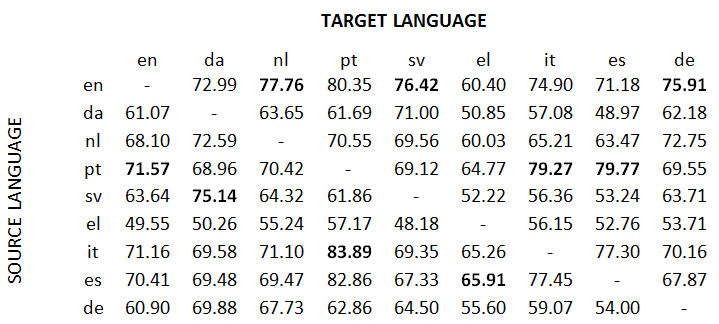
\includegraphics[scale=0.7]{Figures/Prediction}
    \begin{tabular}{rcccccccccc}

          & \multicolumn{10}{c}{TARGET LANGUAGE} \\

    \multicolumn{1}{c}{\multirow{10}[0]{*}{	
    \begin{sideways}  
    SOURCE LANGUAGE
    \end{sideways}
}} &       & en    & da    & nl    & pt    & sv    & el    & it    & es    & de \\
    \multicolumn{1}{c}{} & en    & -     & 72.99 & \textbf{77.76} & 80.35 & \textbf{76.42} & 60.40 & 74.90 & 71.18 & \textbf{75.91} \\
    \multicolumn{1}{c}{} & da    & 61.07 & -     & 63.65 & 61.69 & 71.00 & 50.85 & 57.08 & 48.97 & 62.18 \\
    \multicolumn{1}{c}{} & nl    & 68.10 & 72.59 & -     & 70.55 & 69.56 & 60.03 & 65.21 & 63.47 & 72.75 \\
    \multicolumn{1}{c}{} & pt    & \textbf{71.57} & 68.96 & 70.42 & -     & 69.12 & 64.77 & \textbf{79.27} & \textbf{79.77} & 69.55 \\
    \multicolumn{1}{c}{} & sv    & 63.64 & \textbf{75.14} & 64.32 & 61.86 & -     & 52.22 & 56.36 & 53.24 & 63.71 \\
    \multicolumn{1}{c}{} & el    & 49.55 & 50.26 & 55.24 & 57.17 & 48.18 & -     & 56.15 & 52.76 & 53.71 \\
    \multicolumn{1}{c}{} & it    & 71.16 & 69.58 & 71.10 & \textbf{83.89} & 69.35 & 65.26 & -     & 77.30 & 70.16 \\
    \multicolumn{1}{c}{} & es    & 70.41 & 69.48 & 69.47 & 82.86 & 67.33 & \textbf{65.91} & 77.45 & -     & 67.87 \\
    \multicolumn{1}{c}{} & de    & 60.90 & 69.88 & 67.73 & 62.86 & 64.50 & 55.60 & 59.07 & 54.00 & - \\

    \end{tabular}%

\caption{Predicted Tagger Accuracy for each source-target language pair. The best predicted tagger for each target language is in bold }
\label{fig:taggerPerformancePredicted}
\end{table}

We evaluate our model in a leave-one-out cross validation experiment. To build a predictive model for language $t$, we remove data in Table~\ref{fig:taggerPerformance} associated with $t$ and train the multiple linear regression model $model(t)$ on the remaining data. So, given source language $s$ and $(s-t)$ parallel data sets, $model(t)$ outputs the predicted performance of the tagger trained on $(s-t)$ parallel data sets. The predicted accuracy for each language pair is given in Table \ref{fig:taggerPerformancePredicted}. However, the correlation of the predicted value (Table \ref{fig:taggerPerformancePredicted}) with the original value (Table~\ref{fig:taggerPerformance}) is very high ($r=0.81$). 

We also build another predictive model based solely on monolingual features (morphology complexity and language relatedness). The intuition here is that, if we only have monolingual data and we are planning to build a tagger for target language $t$, what parallel data would we want to collect first? This monolingual model also shows a high correlation with the original table ($r=0.74$). If we only use language relatedness, the correlation is very weak ($r=0.13$), showing that language relatedness on its own is not effective at predicting the best source language.

The predicted best source language for each target language $t$ is the language predicted to produce the highest accuracy tagger. For example, from Table \ref{fig:taggerPerformancePredicted}, if we want to build a tagger for Danish (da), we will choose Swedish (sv) as the source language. Table~\ref{tbl:sourceLangPrediction} shows the source language prediction from models exploiting all features, and only monolingual features. The Fixed model always chooses Dutch (nl) as the source language, because Dutch gives the highest average accuracy (Table~\ref{fig:taggerPerformance}). The Oracle model always picks the best language, and gives the upper bound for the predictive model as a point of comparison. As expected, the model exploiting all features achieves a higher average accuracy than the monolingual model, which nevertheless still outperforms Fixed. With respect to the oracle upperbound, and Fixed baseline, the error rate reduction for the monolingual and all features models is 10.9\% and 52.3\%, respectively, showing the effectiveness of using a predictive model.


\begin{table}
\small
\centering
    \begin{tabular}{cccc|c}
    Target language & All features & Monolingual features & Fixed& Oracle\\\hline
    en              & pt (72.40)          & \textbf{nl (75.70)} & \textbf{nl (75.70)}& nl (75.70) \\ 
    da              & sv  (75.82)          & en (76.17)  & \textbf{nl (76.31)} &  nl (76.31)\\
    nl              & \textbf{en  (72.97)}              & \textbf{en (72.97)}&  - & de (76.54)\\
    pt              & \textbf{it  (84.50)}           & es (80.72)& nl (78.92
) & it (84.50)\\
    sv              & \textbf{en  (73.83)}               & \textbf{en (73.83)} & nl (70.24) & en (73.83)\\
    el              & \textbf{es  (62.29)}            & en (50.38)& nl (54.22) & es  (62.29) \\
    it              & \textbf{pt  (74.23)}          & es (74.07) & nl (70.49) & pt  (74.23) \\
    es              & \textbf{pt   (80.50)}          & \textbf{pt (80.50)}  & nl (76.90) & it (81.80)\\
    de              & en  (73.95)         & en (73.95)  & \textbf{nl (79.47)} & nl (79.47)\\ \hline
    Average         & \textbf{ \phantom{xx (}74.50\phantom{)} }     & \phantom{xx (}73.14\phantom{)}& \phantom{xx (}72.78\phantom{)} & \phantom{xx (}76.07\phantom{)}
    \end{tabular}
    \caption{Best source language prediction (and corresponding tagger performance) for models exploiting all features, only monolingual features, and a fixed source language, as well as an oracle model that always picks the best language. The best (non-oracle) source language and accuracy for each target language is shown in bold.}
    \label{tbl:sourceLangPrediction}
\end{table}

% MULTIPLE SOURCE LANGUAGES 
\section{Multiple Source Languages}
\label{sec:multipleSourceLanguages}


\begin{figure}
\centering
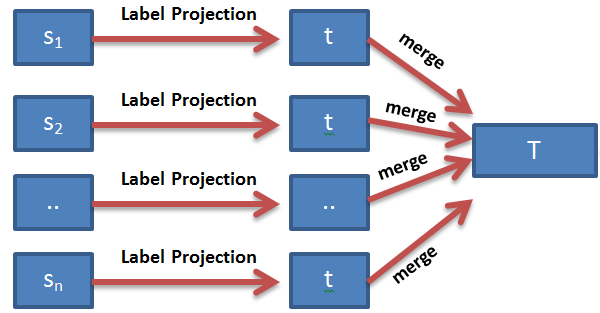
\includegraphics[scale=0.7]{Figures/multiSource}
\caption{Combining multiple source language to produce single file }
\label{fig:multipleSource}
\end{figure}

%% PC: Need to update notation in Figure to match text.
%% LD: Done
In this section we combine information from multiple source languages
to build a single target language tagger. We take a simple approach as shown in Figure \ref{fig:multipleSource}. Each $s_i$ is a
tagged corpus for source language $i$. POS tags are then projected to
the target language side $t$ for each corpus. We merge all of these
partially-tagged target language corpora (in which unaligned words are
untagged) to form $T$. Because the JRC-Acquis corpus consists
  of translations of documents into multiple languages, in many cases
  the same target language sentence occurs in the parallel corpus for
  multiple source languages. In this preliminary approach to combining
  information from multiple source languages, we simply treat these as
  different target language sentences because the sentences are
  aligned with different source languages, they might contain
  different partial tag information.  
  
We build the target language tagger from $T$ by adapting the method from chapter
\ref{chap:uniTagger} (Universal Tagger). The typical steps for this method are (1) tag the source language, (2) project labels from the source to target
language, (3) build the seed model, and (4) apply self-training with
revision to produce the final model. Here we simply start from step
(3) and build the seed model from $T$.

 \begin{table}
 \centering
     \begin{tabular}{clllllll}
     Language    & 1 best & 2 best      & 3 best       & 4 best       & 5 best       & 6 best       & 7 best      \\\hline
     en      &    75.70    &    76.36 &    76.66 &    77.17 &    76.36 &    77.06 &    \textbf{78.16} \\
     da      &    76.31    &    78.06 &    78.40 &    \textbf{83.35} &    82.45 &    82.60 &    82.43 \\
     nl      &    76.54    &    76.82 &    76.17 &    76.03 &    80.00 &    \textbf{81.60} &    81.45 \\
     pt      &    84.50    &    83.84 &    84.91 &    84.79 &    85.00 &    \textbf{85.46} &    84.24 \\
     sv      &    73.83    &    74.33 &    74.65 &    74.49 &    74.10 &    74.51 &    \textbf{76.66 }\\
     el      &    62.29    &    66.90 & \textbf{ 70.23} &    67.93 &    67.22 &    67.03 &    67.69 \\
     it      &    74.23    &    77.28 &    \textbf{78.71} &    78.47 &    78.47 &    78.03 &    76.05 \\
     es      &    81.80    &    81.89 &    82.53 &    \textbf{82.76} &    82.13 &    82.21 &    82.64 \\
     de      &  \textbf{  79.47}    &    79.35 &    79.28 &    78.79 &    77.92 &    77.88 &    77.35 \\\hline
     Average &    76.07    &    77.20 &    77.95 &    78.20 &    78.18 &    78.49 &    \textbf{78.52} \\
     Run time(s) & 352 & 444 & 741 & 1025 & 1648 & 2790 & 3297
     \end{tabular}    \caption{Tagger performance when combine multiple source language and performance of Portuguese languages measured in seconds. The best system are in bold }
     \label{tbl:multipleSource}
 \end{table}

%\begin{table}
%\small
%\centering
%    \begin{tabular}{lrrrr}
%    Language    & 1-best       & 3-best         & 5-best         &  7-best      \\
%\hline
%    en      &    75.70         &    76.66       &    76.36       &     \textbf{78.16} \\
%    da      &    76.31         &    78.40       & \textbf{82.45} &     82.43 \\
%    nl      &    76.54         &    76.17       &    80.00       &     \textbf{81.45} \\
%    pt      &    84.50         &    84.91       &    \textbf{85.00}       &     84.24 \\
%    sv      &    73.83         &    74.65       &    74.10       &     \textbf{76.66 }\\
%    el      &    62.29         & \textbf{70.23} &    67.22       &     67.69 \\
%    it      &    74.23         & \textbf{78.71} &    78.47       &     76.05 \\
%    es      &    81.80         &    82.53       &    82.13       &     \textbf{82.64} \\
%    de      &  \textbf{79.47}  &    79.28       &    77.92       &     77.35 \\
%\hline
%    Average &    76.07         &    77.95       &    78.18 &     \textbf{78.52} \\
%    %% Run time(s) & 352 & 741 & 1648 & 3297\\
%    \end{tabular}
%    \caption{Tagger accuracy when combining the 1-, 3-, 5-, and 7-best
%      source languages. The best system for each target language is shown in
%      bold.}
%    \label{tbl:multipleSource}
%\end{table}

In these experiments we assume that when building a tagger for a
target language we have access to all other source languages. Table
\ref{tbl:multipleSource} shows accuracy when combining information
from the \mbox{1-,} \mbox{2-,} \mbox{3-,} to 7-best source languages
(where the best source language is determined by an oracle). As more
source languages are added, the average accuracy increases, although
there is some variation for individual languages. Nevertheless, these
findings show that the method described in chapter \ref{chap:uniTagger} is robust and can be substantially improved by combining information from multiple source
languages. There is, however, a trade-off between accuracy and
efficiency, with taggers built from multiple source languages
generally being slower.
The memory and running time is $O(nlogn)$ with the amount of data $n$. Table \ref{tbl:multipleSource} also shows the running time for
 Portuguese on each combination. We run our experiment on a 16 cores Intel Xeon 2.53 GHz server with 24GB RAM. 
%% We assume that when building tagger for target language we have all
%% other source languages available. Table \ref{tbl:multipleSource} show
%% the tagger performance when combining the single best, 2 best, 3 best,
%% 4 best, 5 best, 6 best and 7 best source languages. Table
%% \ref{tbl:multipleSource} confirms the robustness of \cite{Duong:2013}
%% method. As more data are added, it introduced more noise, however, in
%% general, the model handles it well as average performance
%% increased. The memory and running time is $O(nlogn)$ with the amount
%% of data $n$. Table \ref{tbl:multipleSource} shows the running time for
%% Portuguese on each combination. We ran our experiment on a Intel(R)
%% Xeon(R) 2.53GHz server with 24GB RAM . The running time is measured in
%% seconds. Therefore, as the trade-off between performance and
%% computational complexity, we would prefer using just 4 best
%% systems. Out of 9 languages, using up to 4 best source language give
%% us the best performance for 5 languages. On average, 4 best option
%% achieves competitive result but remain fast. For the best accuracy, we
%% would use all possibles source languages.

\section{Summary of Contributions}

In this chapter, we investigated the problem of choosing the best
source language(s) to use in unsupervised multilingual POS tagging based
on tag projection in parallel corpora. We have shown that our predictive model can select a source language --- based on only monolingual features of the source and
target languages --- that improves tagger accuracy compared to
choosing the single best (overall) source language. However, if
parallel data is available, our predictive model is able to leverage
this to select a more appropriate source language and obtain further
improvements in accuracy. Finally, we showed that if multiple source
languages are available, even better accuracy can be obtained by
combining information from just those sources that are selected by our model. A synopsis of the process for building a tagger for language $S$ is described in Figure \ref{fig:cheatSheet}. That is, if we do not have any parallel data, we would use a monolingual model to predict the best source language $T$ and collect $S-T$ parallel data sets. If multiple parallel data sets are available and we have time, the best solution is just to combine all source languages to produce the single best tagger. If we do not have time, just combine $n$-best source languages in the order defined by \textit{all features model} gave the comparable accuracy but stay fast. 

\begin{figure}
\centering
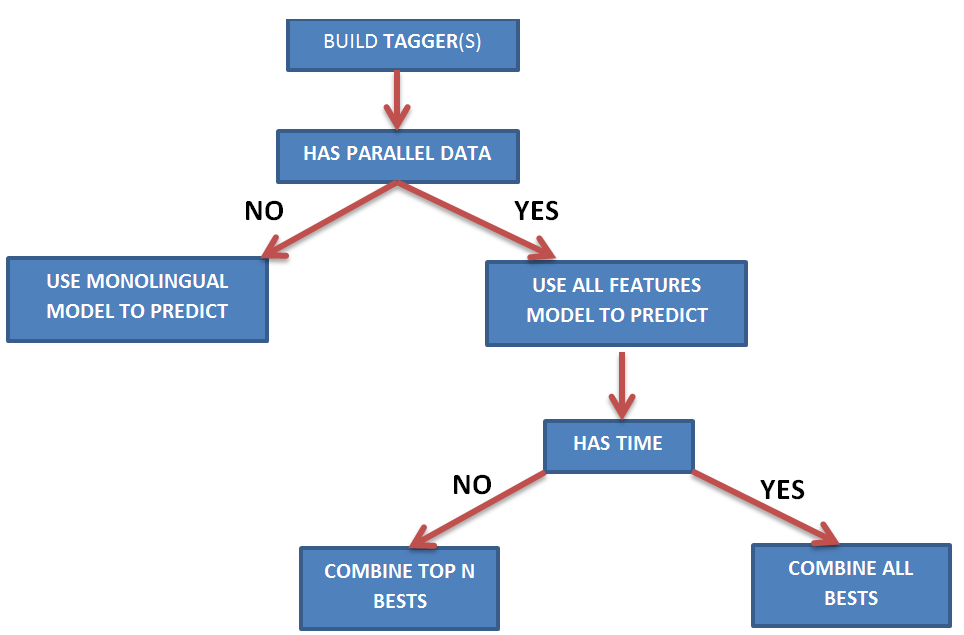
\includegraphics[scale=0.5]{Figures/cheatSheet}
\caption{Instruction for building tagger for target language $S$}
\label{fig:cheatSheet}
\end{figure}

In future work, we would like to apply the methods described in this
paper for identifying ``good'' source languages for other multilingual
NLP tasks which exploit parallel data to transfer annotations between
languages, including grammar induction, parsing, and morphological
analysis. We further intend to expand our experiments to consider more
source and target languages. We also would like to investigate more methods for combining different source languages. Currently, we ignore cross-language sentences and concatenate them without any further processing. This resource can be very valuable since we have the POS information from all other languages for each individual sentence. Thus, we can combine and produce more accurate tagged sentences which will serve as better training data for the POS tagger. 
%% To the best of our knowledge, we are first quantifying the question
%% ``which is the best source language for a target POS tagger". Our
%% predicting model which build just on monolingual features has proved
%% to be useful and very easy to build. We also gave thoroughly analysis
%% about the performance of multiple source languages. In summary, if we
%% don't have any parallel data, we will use our monolingual predicting
%% model to predict the source language. If we have parallel data, the
%% best thing to do is just combining all of them. In the future, we
%% would like to testify our methods on other multilingual natural
%% language processing(NLP) tasks which exploiting parallel data to copy
%% annotated label from source to target language. These tasks might be,
%% grammar induction, parsing, morphology analysis etc. We also would
%% like to expand this experiment to other languages. This way, we can
%% make a bigger matrix ranking source language for each target language.




% Chapter 5: Summary and Future work
%%% CHAPTER 5 

\chapter{Conclusions}

\label{chap:conclusion}
POS tagging is an important task as it gives syntactic information and also helps to differentiate semantic information. There are three main challenges for POS tagging, (1) lack of manually annotated data which makes supervised approach impossible for resource-poor languages; (2) low performance on the traditional unsupervised approach which looks at each language separately; and (3) lack of tagset consensus among languages which is an obstacle for cross-language processing. In this thesis we tackle these challenges. We have successfully built an unsupervised multilingual POS tagger, but additionally, exploiting parallel data to copy tag information from resource-rich to resource-poor languages. In our tagger, we also employ the Consensus 12 Universal Tagset across languages which will resolve the third challenge. 

Chapter \ref{chap:backGround} thoroughly reviewed approaches for POS tagging for both monolingual and multilingual taggers. Chapter \ref{chap:uniTagger} proposed the initial method for building Universal Tagger. That is, given a source language tagger and parallel data, we successfully construct a target language tagger. This tagger performs on par with the state-of-the-art system for the same 8 languages \cite{Das:2011}. However, we use less data, simper methods -- i.e. a huge difference in running speed, easier to replicate which actually makes our proposed method stronger. Unlike \namecite{Das:2011}, we are able to publish the implementation\footnote{https://code.google.com/p/universal-tagger/} which might aid other researchers not only in multilingual POS tagging but also on other cross-languages NLP tasks such as parsing, grammar induction and so forth. 

Out of 8 languages, the  Universal Tagger performs better than the state-of-the-art on 4 Germanic languages which are in the same family as source language (English). It appears that choice of source language might substantially affect the target language tagger. This idea motivates our work in chapter \ref{chap:sourceLanguageSelection}. This chapter is the effort to further improve unsupervised multilingual POS tagger (Universal Tagger) accuracy by investigating the effect of choosing better source language(s). We found out that English is usually not the best source language.  Just based on monolingual features, we are able to predict the best source language for a given target language. On average, the source language prediction gave better tagger performance than always fixing the source language. Even better accuracy can be obtain if we have parallel data. When multiple source languages are available, we shown that combining all of them even further improve tagging accuracy. 

This thesis described a consensus works and thoroughly analysis of many aspects of building unsupervised multilingual POS tagger. Nevertheless, there are many points that could be improved. The program for future research is divided into 3 categories: (1) immediate works, which require less effort and can be done in few weeks; (2) near future works, which might require few months to complete; and (3) longer future works, which require years to complete. 
\subsubsection{Immediate works}
\begin{enumerate}
\itemsep0pt
\item Use a larger and more diverse traning corpus. 

The Universal Tagger we constructed in chapter \ref{chap:uniTagger} only uses the Europarl parallel corpus~\cite{europarl}. Whereas the state-of-the-art~\cite{Das:2011} additionally uses the ODS United Nations data set. Thus, we would like to acquire this corpus and add to the current Universal Tagger. This way, our model and the state-of-the-art will become fully comparable. Moreover, the current high rate of unknown word (OOV) when evaluating Universal Tagger against 8 languages suggested that enlarging the corpus might be the easiest and most promising way to improve performance. 

\item Try bidirectional alignments

Alignment is the one of the core modules of our Universal Tagger. Currently, we only employ one directional alignment from source to target language. It is possible to align in another direction from target to source language and then merge the results from these two alignments. In this way, we might have more and even better alignments. Actually, bidirectional alignment is widely used in statistical machine translation systems i.e. Moses~\cite{Koehn:2007:MOS}. We acknowledge this idea beforehand. However, alignment is the most time-consuming step in our model, bidirectional alignment doubles the running time, thus, we leave it for future work. 

\item Build predicting model for many more languages

This is a trivial extension of chapter \ref{chap:sourceLanguageSelection}. Currently, we are able to build a predicting model that predicts best source language given target language for 9 European languages, i.e. English, Dutch, Danish, German, Greek, Italian, Portuguese, Spanish, Swedish. We distinguish between two predicting models, that is, a \emph{monolingual model} which just exploits monolingual data and an \emph{all features model} which additionally exploits parallel data. We would like to extend this to more languages, in a different strategy. First, for all 22 European languages in the JRC-Acquis Corpus ~\cite{SteinbergerAcquis}, we have parallel data for each language pair, thus, we will build \emph{all feature model} for better prediction. Second, we can further expand to more languages by just exploiting a \textit{monolingual model} which only needs monolingual data. For example, we can easily build \textit{monolingual model} for all languages presented in Wikipedia. 

\end{enumerate}

\subsubsection{Near future works}
\begin{enumerate}
\itemsep0pt
\item Investigate methods for handling unknown word (OOV) case.

As mentioned above, OOV rate stays high (nearly 10\%) when evaluating the Universal Tagger on 8 languages. Currently, for unknown words (OOV), the model just uses the tag sequence to predict. For example, the tag sequence ``\textit{DET ADJ NOUN}" is commonly observed. So, if two previous words of unknown word are tagged as \textit{DET} and \textit{ADJ}, model infers \textit{NOUN} for this word. The performance of this method on unknown words varies between languages but stays quite low i.e. 50-60\% for Italian (Figure \ref{fig:italian}, page \pageref{fig:italian}). Thus, given the high rate and currently low performance on OOV words, if we can incorporate other evidences to have better prediction for unknown words, we hope to improve the final performance. 

\item Implement HMM inference algorithms

We can use the Universal Tagger to initialize the first state of a Hidden Markov Model (HMM) and then use inference algorithms such as  Expectation Maximization (EM),  Variational Bayes (VB) or Gibbs Sampling (GS) to estimate the new set of parameters (emission probability and transition probability).~\namecite{Gao:2008} compare EM, VB and GS for the same task of POS tagging, it seems that GS outperforms EM and VB. Thus, we would like to try GS first for our model. 

\item Investigate more on combining multiple resources algorithms

Chapter \ref{chap:sourceLanguageSelection} shows that combining multiple source languages improves the overall accuracy. The current combining scheme is just concatenation, that is, ignore the existence of sentences that are shared among all languages. Thus, we would like to investigate methods that treat these sentences separately and propose a better combining scheme. 
\end{enumerate}

\subsubsection{Longer future works}

Our experience with parallel data, alignment, label projection, etc. will be the advantage for investigating similar unsupervised cross-language NLP tasks such as parsing, name entity recognition, noun phrase bracketing etc. The first task we would like to investigate is sentence parsing which is built upon POS information. However the ultimate goal for this thread of work is building a framework for resource-poor languages, exploiting parallel data as the bridge between resource-rich and resource-poor languages. After being able to build another cross-lingual NLP applications, we would like to verify the source language predictive model proposed in Chapter \ref{chap:sourceLanguageSelection} against these other applications. 




% bibliography:
\footnotesize
%%% bibliography for thesis.
\bibliography{References}
\bibliographystyle{aclnat}

%\nocite{}
%
%{
%\ssp % single-spacing
%
%\bibliography{References}
%\bibliographystyle{aclnat}
%}

\normalsize
%\appendix
%\chapter{Other Papers}
%this is other chapter
%\chapter{}
\label{section:appendixA}
%\renewcommand{\baselinestretch}{0.3}
\begin{table}
  \centering
  \scalebox{1.0}{
    \begin{tabular}{cll}
    \multicolumn{1}{c}{\textbf{POS Tag}} & \multicolumn{1}{c}{\textbf{Description}} & \multicolumn{1}{c}{\textbf{Example}} \\\hline

    CC    & coordinating conjunction & and \\
    CD    & cardinal number & 1, third \\
    DT    & determiner & the \\
    EX    & existential there & there is \\
    FW    & foreign word & d'hoevre \\
    IN    & preposition/subordinating conjunction & in, of, like \\
    JJ    & adjective & green \\
    JJR   & adjective, comparative & greener \\
    JJS   & adjective, superlative & greenest \\
    LS    & list marker & 1) \\
    MD    & modal & could, will \\
    NN    & noun, singular or mass & table \\
    NNS   & noun plural & tables \\
    NNP   & proper noun, singular & John \\
    NNPS  & proper noun, plural & Vikings \\
    PDT   & predeterminer & both the boys \\
    POS   & possessive ending & friend's \\
    PRP   & personal pronoun & I, he, it \\
    PRP\$ & possessive pronoun & my, his \\
    RB    & adverb & however, usually \\
    RBR   & adverb, comparative & better \\
    RBS   & adverb, superlative & best \\
    RP    & particle & give up \\
    TO    & to    & to go, to him \\
    UH    & interjection & uhhuhhuhh \\
    VB    & verb, base form & take \\
    VBD   & verb, past tense & took \\
    VBG   & verb, gerund/present participle & taking \\
    VBN   & verb, past participle & taken \\
    VBP   & verb, sing. present, non-3d & take \\
    VBZ   & verb, 3rd person sing. present & takes \\
    WDT   & wh-determiner & which \\
    WP    & wh-pronoun & who, what \\
    WP\$  & possessive wh-pronoun & whose \\
    WRB   & wh-abverb & where, when \\
    \end{tabular}}%
  \caption{Penn Treebank Tagset \protect\cite{PenTreeBank}}
  \label{tab:addlabel}%
\end{table}%


% insert other appendices here...

\end{document}
